\documentclass[a4paper]{report}

\usepackage[utf8]{inputenc}
\usepackage[english]{babel}
\usepackage[T1]{fontenc}
\usepackage{textcomp}
\usepackage[]{amsthm} 
\usepackage[]{amssymb}
\usepackage{amsmath}
\usepackage{graphicx}
\usepackage{float}
\usepackage{soul}
\usepackage{color}
\usepackage{bm}
\usepackage{listings}
\usepackage[table]{xcolor}
\usepackage{enumitem}
%\usepackage{xfrac}
\usepackage[normalem]{ulem}
\usepackage{subcaption}
\usepackage[colorlinks=true, linkcolor=blue]{hyperref}

\usepackage{tikz}
\usetikzlibrary{trees}
\usetikzlibrary {fit,shapes.geometric} % W: Command terminated with space. (1)
\usetikzlibrary {automata} % W: Command terminated with space. (1)
\usetikzlibrary{arrows.meta}
\usepackage{multicol}

\usepackage{algorithm}
\usepackage[noend]{algpseudocode}
\usepackage{caption}

\usepackage{pgfplots}
\pgfplotsset{compat = newest}

\usepackage{geometry}
\geometry{legalpaper, margin=1in}

\renewcommand{\labelitemii}{$\circ$}
\renewcommand{\labelitemiii}{$\star$}
\renewcommand{\labelitemiv}{$>$}

%\renewcommand{\thesection}{} % overwrites section numbering
%\renewcommand{\thesubsection}{} % overwrites section numbering

% figure support
\usepackage{import}
\usepackage{xifthen}
\pdfminorversion=7
\usepackage{pdfpages}
\usepackage{transparent}
\newcommand{\incfig}[1]{%
    \def\svgwidth{\columnwidth}
    \import{./figures/}{#1.pdf_tex}}

% Newline for algorithm psuedo
\newcommand{\algrule}[1][.2pt]{\par\vskip.5\baselineskip\hrule height #1\par\vskip.5\baselineskip}

% -------- Listings/XColor Settings --------
\definecolor{codegreen}{rgb}{0,0.6,0}
\definecolor{codegray}{rgb}{0.5,0.5,0.5}
\definecolor{codepurple}{rgb}{0.58,0,0.82}
\definecolor{backcolour}{rgb}{0.95,0.95,0.92}

\lstdefinestyle{mystyle}{
	backgroundcolor=\color{backcolour},
	commentstyle=\color{codegreen},
	keywordstyle=\color{magenta},
	numberstyle=\tiny\color{codegray},
	stringstyle=\color{codepurple},
	basicstyle=\ttfamily\footnotesize,
	breakatwhitespace=false,
	breaklines=true,
	captionpos=b,
	keepspaces=true,
	numbers=left,
	numbersep=5pt,
	showspaces=false,
	showstringspaces=false,
	showtabs=false,
	tabsize=2,
	float=H
}

\lstset{style=mystyle}

% -------------- Doc Start -------------------



\pdfsuppresswarningpagegroup=1

\title{\Huge{Revisit to CPE233 (Digital Design)}}
\author{\textbf{Authors:} \\WhisperingRock \\ \\ \textbf{Professor:} \\}
\date{Class\\ \small{Quarter} \\ \today}

\begin{document}
    \maketitle
	\addcontentsline{toc}{section}{Contents}
	\tableofcontents
	\newpage

	Note : All assignments are in the \textbf{CPE 233 Lab Manual}.

	\section{Hardware}

		\subsection{HW1 - Program ROM}

			\subsubsection{Reverse Engineer'd Table}

				\begin{figure}[H]
					\centering
					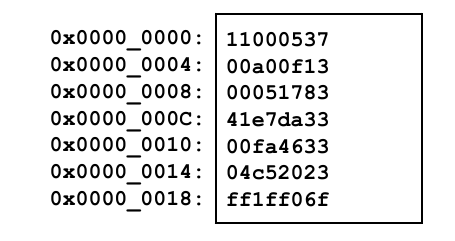
\includegraphics[width=0.5\textwidth]{../03_hardware/hw1/photos/given.png}
					\caption{Which Table? This table}
					\label{fig:hw1_table}
				\end{figure}

				\begin{figure}[H]
					\centering
					\includegraphics[width=0.8\textwidth, page=732]{../00_books/Digital Design and Computer Architecture RISC-V Edition (Sarah Harris, David Harris) (Z-Library).pdf}
				\end{figure}

				\begin{table}[H]
					\centering
					\begin{tabular}{||c|c|c|c||}
						\hline
						\textbf{ProgROM Addr} & \textbf{Machine Code} & \textbf{Type} & \textbf{Assembly Instruction} \\\hline
						0000 & \tiny{0x1100 0537} & & \\ \hline
							 & \tiny{0001 0001 0000 0000 0000 0101 0\colorbox{yellow}{011 0111}} & (55) U  & \texttt{lui rd, upimm}\\ \hline
							 & \tiny{\colorbox{lightgray}{0001 0001 0000 0000 0000} \colorbox{cyan}{0101 0}011 0111} & (55) U  & \texttt{lui \colorbox{cyan}{x10}, \colorbox{lightgray}{0x11000}}\\ \hline

						0004 & \tiny{0x00A0 0F13} & & \\ \hline
							 & \tiny{0000 0000 1010 0000 0\colorbox{green}{000} 1111 0\colorbox{yellow}{001 0011}} & (19)I & \texttt{addi rd, rs1, imm}\\ \hline
							 & \tiny{\colorbox{lightgray}{0000 0000 1010} \colorbox{orange}{0000 0}000 \colorbox{cyan}{1111 0}001 0011} & (19)I & \texttt{addi \colorbox{cyan}{x30}, \colorbox{orange}{x0}, \colorbox{lightgray}{0x00A}}\\ \hline

						0008 & \tiny{0x0005 1783} & & \\ \hline
							 & \tiny{0000 0000 0000 0101 0\colorbox{green}{001} 0111 1\colorbox{yellow}{000 0011}} & (3)I & \texttt{lh rd, imm(rs1)}\\ \hline
							 & \tiny{\colorbox{lightgray}{0000 0000 0000} \colorbox{orange}{0101 0}001 \colorbox{cyan}{0111 1}000 0011} & (3)I & \texttt{lh \colorbox{cyan}{x15}, \colorbox{lightgray}{0}(\colorbox{orange}{x10})}\\ \hline

						000C & \tiny{0x41E7 DA33} & & \\ \hline
							 & \tiny{\colorbox{magenta}{0100 000}1 1110 0111 1\colorbox{green}{101} 1010 0\colorbox{yellow}{011 0011}} & (51)R & \texttt{sra rd, rs1, rs2}\\ \hline
							 & \tiny{0100 000\colorbox{lime}{1 1110} \colorbox{orange}{0111 1}101 \colorbox{cyan}{1010 0}011 0011} & (51)R & \texttt{sra \colorbox{cyan}{x20}, \colorbox{orange}{x15}, \colorbox{lime}{x30}}\\ \hline

						0010 & \tiny{0x00FA 4633} & & \\ \hline
							 & \tiny{0000 0000 1111 1010 0\colorbox{green}{100} 0110 0\colorbox{yellow}{011 0011}} & (51)R & \texttt{xor rd, rs1, rs2}\\ \hline
							 & \tiny{0000 000\colorbox{lime}{0 1111} \colorbox{orange}{1010 0}100 \colorbox{cyan}{0110 0}011 0011} &(51)R & \texttt{xor \colorbox{cyan}{x12}, \colorbox{orange}{x20}, \colorbox{lime}{x15}}\\ \hline

						0014 & \tiny{0x04C5 2023} & & \\ \hline
							 & \tiny{0000 0100 1100 0101 0\colorbox{green}{010} 0000 0\colorbox{yellow}{010 0011}} & (35)S & \texttt{sw rs2, imm(rs1)}\\ \hline
							 & \tiny{\colorbox{lightgray}{0000 010}\colorbox{lime}{0 1100} \colorbox{orange}{0101 0}010 \colorbox{lightgray}{0000 0}010 0011} & (35)S &  \texttt{sw \colorbox{lime}{x12}, \colorbox{lightgray}{0x040}(\colorbox{orange}{x10})}\\ \hline

						0018 & \tiny{0xFF1F F06F} & & \\ \hline
							 & \tiny{1111 1111 0001 1111 1111 0000 0\colorbox{yellow}{110 1111}} & (111)J & \texttt{jal rd, label}\\ \hline
							 & \tiny{\colorbox{lightgray}{1111 1111 0001 1111 1111} \colorbox{cyan}{0000 0}110 1111} & (111)J & \texttt{jal \colorbox{cyan}{x0}, \colorbox{lightgray}{-16}}\\ \hline

					\end{tabular}
					\caption{Reverse Engineering \textit{otter\_memory.mem} segment}
					\label{tab:hw_a1_reverseTable}
				\end{table}

				For the last command, some explanation is required here. 
				Consider
				\begin{itemize}
					\item $Imm[20] = B31 = 1$
					\item $Imm[10:1] = B30:B21 = 1111 111 000$
					\item $Imm[11] = B20 = 1$
					\item $Imm[19:12] = B19:B12 = 1111 1111$
					\item $Imm[0]$ is always zero
					\item Therefore,  $Imm = 0x1FFFF0$
				\end{itemize}

				To find the decimal representation, consider adding our
				large negative number to the next highest max. 

				\begin{align*}
					2^{21} - 0x1FFFF0 &= 0x200000 - 0x1FFFF0 \\
					&= -0x10 \\
					&= -16 \\
				\end{align*}	


				BUT WAIT! \texttt{jal} doesn't take immediates, only labels.

				True, our label must be 4 spaces prior to this jump - 
				fill this portion in with a label in the asm and
				respect the spacing. 

				
			\subsubsection{Assembly Code}
				\lstinputlisting[language={[riscv]Assembler}, captionpos=top,
											caption={Assembly of HW1},
											breaklines=false]{../03_hardware/hw1/reverse.asm}

				\begin{figure}[H]
					\centering
					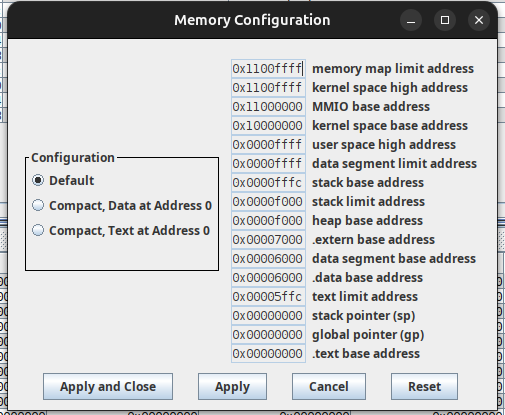
\includegraphics[width=0.5\textwidth]{../03_hardware/hw1/photos/memconfig}
					\caption{Segment Address Config}
					\label{fig:-03_hardware-a1-photos-memconfig}
				\end{figure}

				\begin{figure}[H]
					\centering
					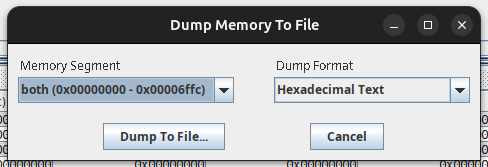
\includegraphics[width=0.5\textwidth]{../03_hardware/hw1/photos/dumpconfig}
					\caption{Memory Dump Config}
					\label{fig:-03_hardware-a1-photos-dumpconfig}
				\end{figure}

				\begin{figure}[H]
					\centering
					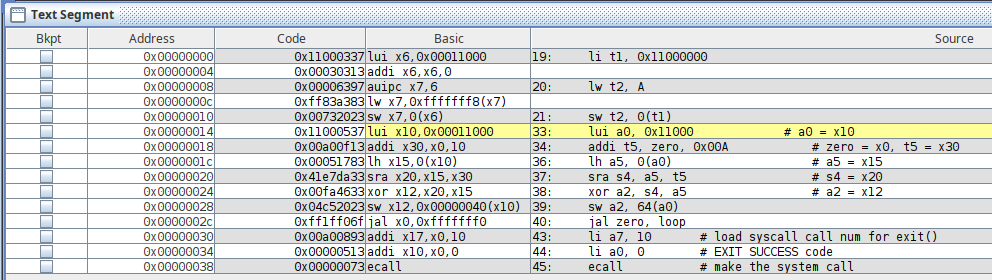
\includegraphics[width=0.8\textwidth]{../03_hardware/hw1/photos/RARS_instr.png}
					\caption{RARS instruction addresses alongside code}
					\label{fig:hw1_rars}
				\end{figure}


			\subsubsection{Vivado Simulation}

				\begin{figure}[H]
					\centering
					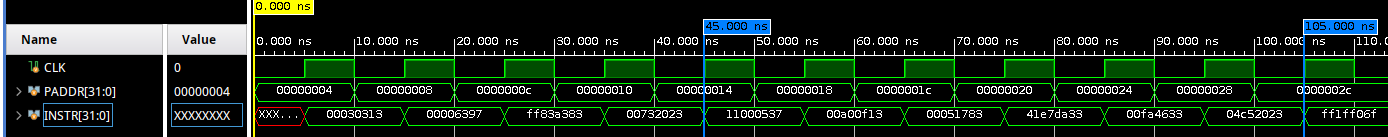
\includegraphics[width=\textwidth]{../03_hardware/hw1/photos/waveform.png}
					\caption{Simulation waveform of \texttt{ProgROM\_tb.sv} running
						\texttt{otter\_memory\_hw1.mem}}
					\label{fig:hw1_waveform}
				\end{figure}

				By inspection, the instructions in the waveform \ref{fig:hw1_waveform}
				match those in RARS\ref{fig:hw1_rars} and our decoded 
				table \ref{tab:hw_a1_reverseTable}
		

		\newpage
		\subsection{HW2 - Program Counter}

			\subsubsection{Intended Behavior(s)}
				\begin{figure}[H]
					\centering
					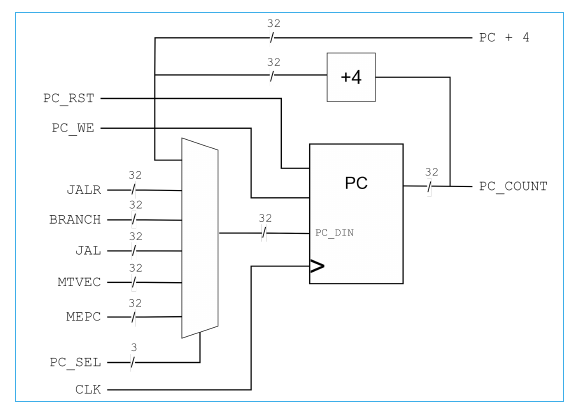
\includegraphics[width=0.6\textwidth]{../03_hardware/hw2/target.png}
					\caption{Program Counter Test Block Design}
					\label{fig:-03_hardware-hw2-target-png}
				\end{figure}

			\subsubsection{Structural Design(s)}
				\begin{figure}[H]
					\centering
					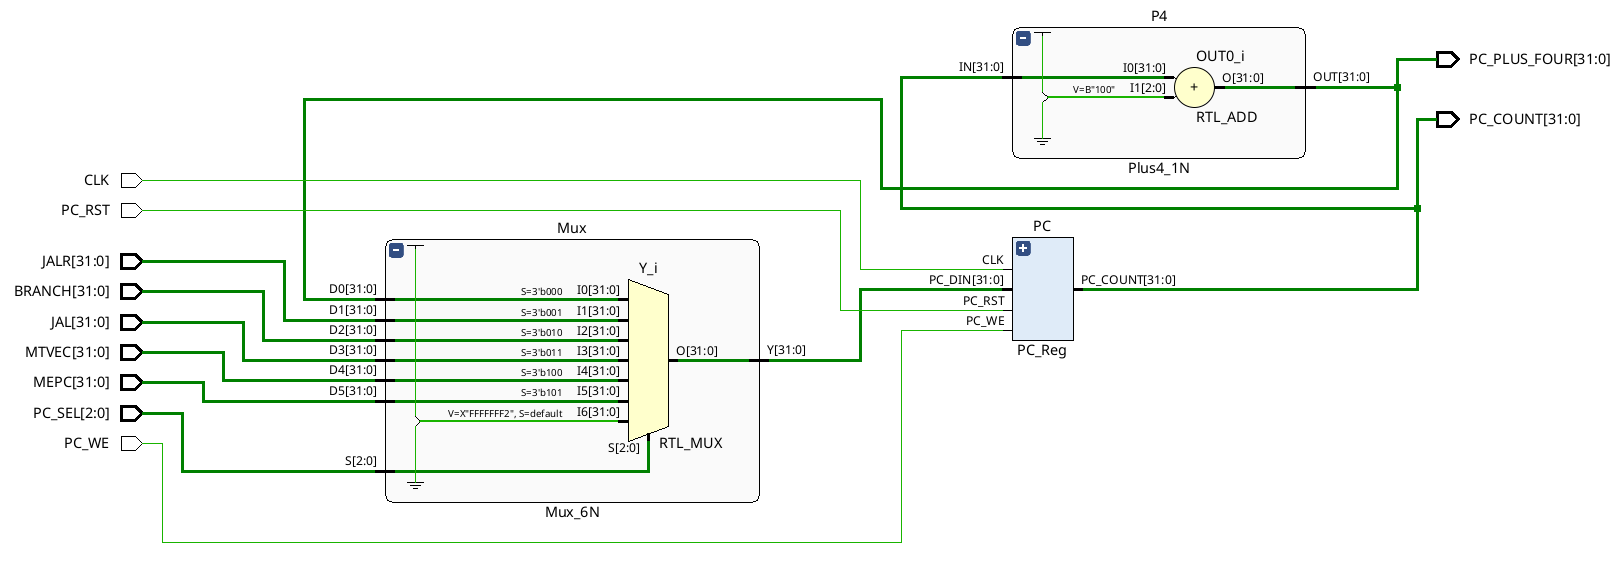
\includegraphics[width=\textwidth]{../03_hardware/hw2/rtl_schematic.png}
					\caption{RTL Design of \texttt{PC\_TestBlock.sv}}
					\label{fig:-03_hardware-hw2-rtl_schematic-png}
				\end{figure}
				
			\subsubsection{Synthesis Warning(s)}
				\begin{figure}[H]
					\centering
					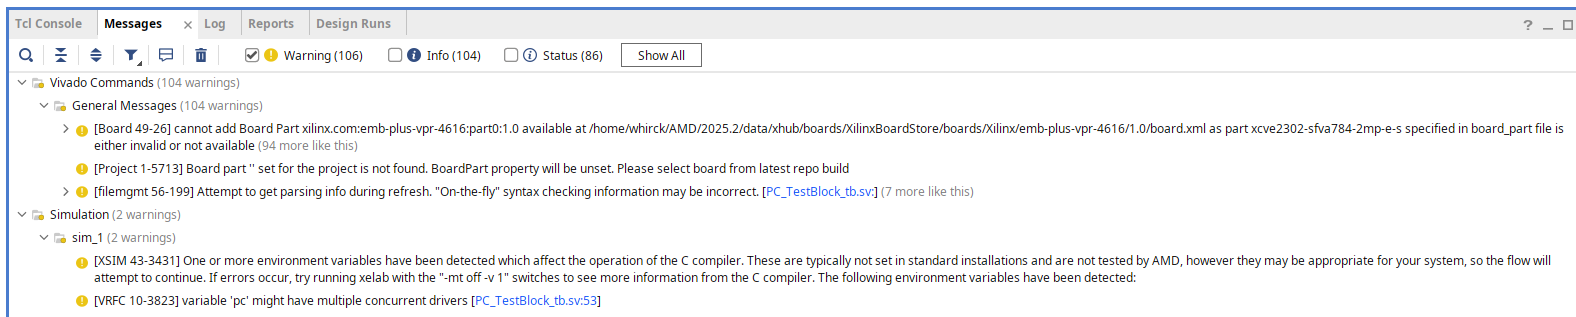
\includegraphics[width=0.8\textwidth]{../03_hardware/hw2/errors.png}
					\caption{Synthesis Errors of \texttt{PC\_TextBlock.sv}}
					\label{fig:-03_hardware-hw2-errors-png}
				\end{figure}

				The only error with importance here is 'clk' having multiple
				concurrent drivers such that one clock toggles clk and 
				the other initially defines the clk value. I opted to proceed
				with this error. 

			\subsubsection{Verification}
				All test cases passed in \texttt{PC\_TestBlock\_tb.sv} passed 
				in simulation along with each subcomponent test bench.  
	
				\lstinputlisting[
					language={Verilog},
					captionpos=top,
					caption={Simulation file for \texttt{PC\_TestBlock.sv}},
					breaklines=false,
					label={fig:pc_tb}
				]{../03_hardware/otter/sim/PC_TestBlock_tb.sv}

				For the 6 Input Mux, see \ref{otter:mux6}

				For the Program Counter register and test file, see
				\ref{otter:pc} and \ref{ottertest:pc}.

			\subsubsection{SystemVerilog Code}

				\lstinputlisting[
					language={Verilog},
					captionpos=top,
					caption={\texttt{PC\_TestBlock.sv}},
					breaklines=false,
					label={fig:pc}
					cite={otter:pc-reg}
				]{../03_hardware/otter/src/PC_TestBlock.sv}

		\newpage
		\subsection{HW3 - Register File}

			\subsubsection{Intended Behavior(s)}
				\begin{figure}[H]
					\centering
					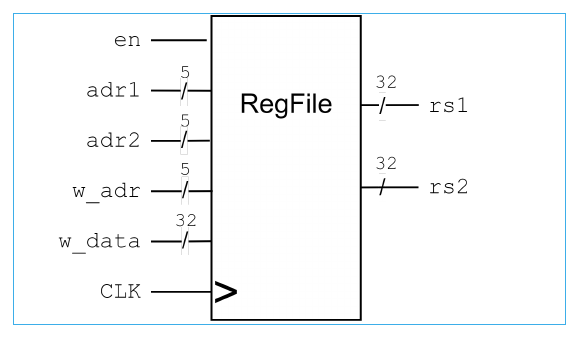
\includegraphics[width=0.6\textwidth]{../03_hardware/hw3/target.png}
					\caption{Top Level Register File}
					\label{fig:-03_hardware-hw3-target-png}
				\end{figure}

				The RAM register file must \ldots
				\begin{itemize}
					\item store 32 32-bit registers
					\item dual asynch fetch the values at ADR1 / ADR2 
							and place them in RS1, RS2
					\item single synch write W\_DATA to W\_ADR if EN is high.
					\item prevent x0 "zero" register from being overwritten.
				\end{itemize}

			\subsubsection{Structural Design(s)}
				\begin{figure}[H]
					\centering
					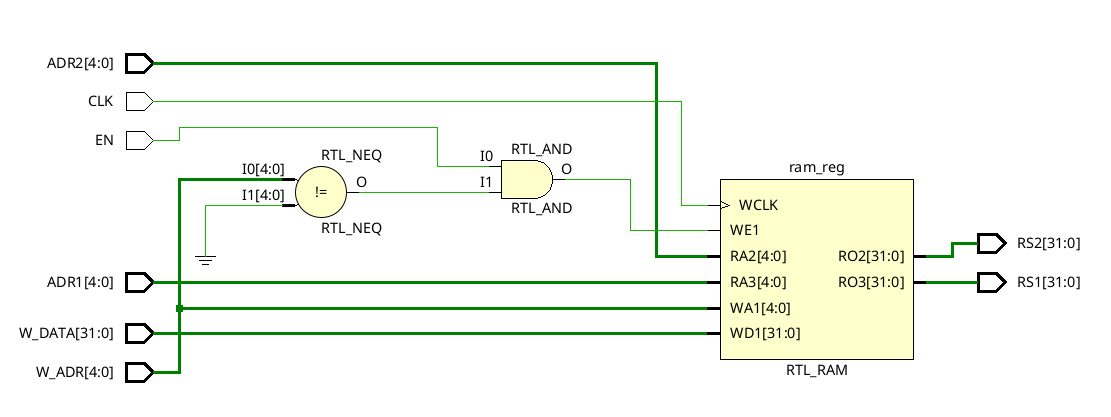
\includegraphics[width=\textwidth]{../03_hardware/hw3/rtl_schematic.png}
					\caption{RTL Design of \texttt{RegFile.sv}}
					\label{fig:-03_hardware-hw3-rtl_schematic-png}
				\end{figure}

				Notice we only overwrite the W\_ADR if EN is high AND 
				W\_ADR is not 0 (for x0).
				
			\subsubsection{Synthesis Warning(s)}
				\begin{figure}[H]
					\centering
					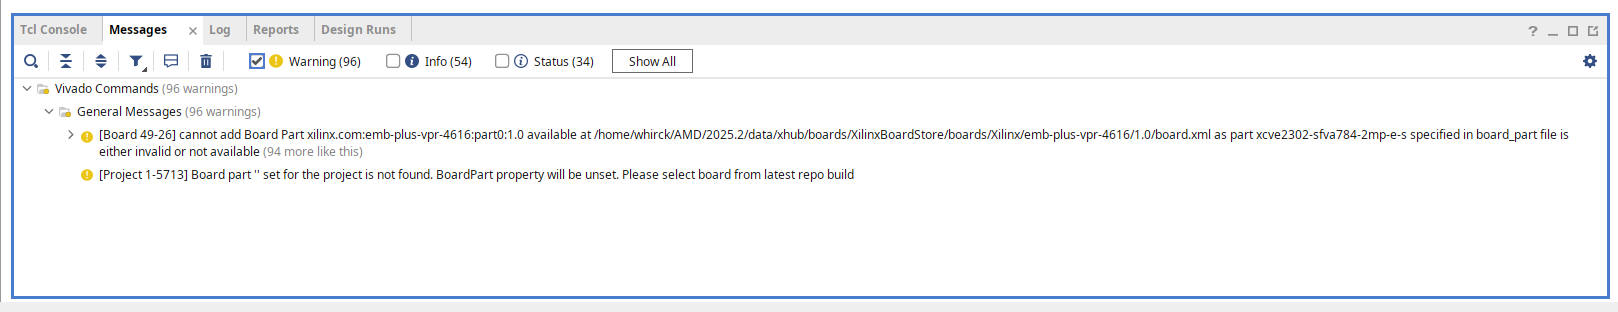
\includegraphics[width=0.8\textwidth]{../03_hardware/hw3/errors.png}
					\caption{Synthesis Errors of \texttt{RegFile.sv}}
					\label{fig:-03_hardware-hw3-errors-png}
				\end{figure}

			\subsubsection{Verification}
				All test cases passed in \texttt{RegFile\_tb.sv} \ref{ottertest:regfile} passed 
				in simulation along with each subcomponent test bench.  
	
			\subsubsection{SystemVerilog Code}

				See \ref{otter:regfile} for the \texttt{RegFile.sv}.

		\newpage
		\subsection{HW4 - ALU + ImmGen}

			\subsubsection{ALU}
				\begin{figure}[H]
					\centering
					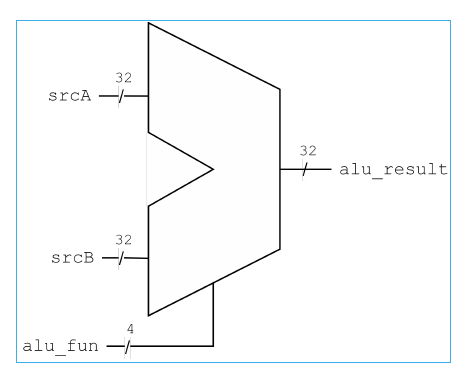
\includegraphics[width=0.5\textwidth]{../03_hardware/hw4/target_alu.png}
					\caption{Top Level ALU}
					\label{fig:-03_hardware-hw4-target_alu-png}
				\end{figure}

				The ALU is designed to perform the arithmetic and logic
				operations required by the RISC-V CPU. Note the 11 
				we implemented here. 

				\begin{figure}[H]
					\centering
					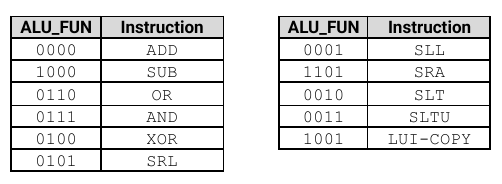
\includegraphics[width=0.6\textwidth]{../03_hardware/hw4/design_alu.png}
					\caption{Instruction Operations of the ALU}
					\label{fig:-03_hardware-hw4-design_alu-png}
				\end{figure}

				\begin{figure}[H]
					\centering
					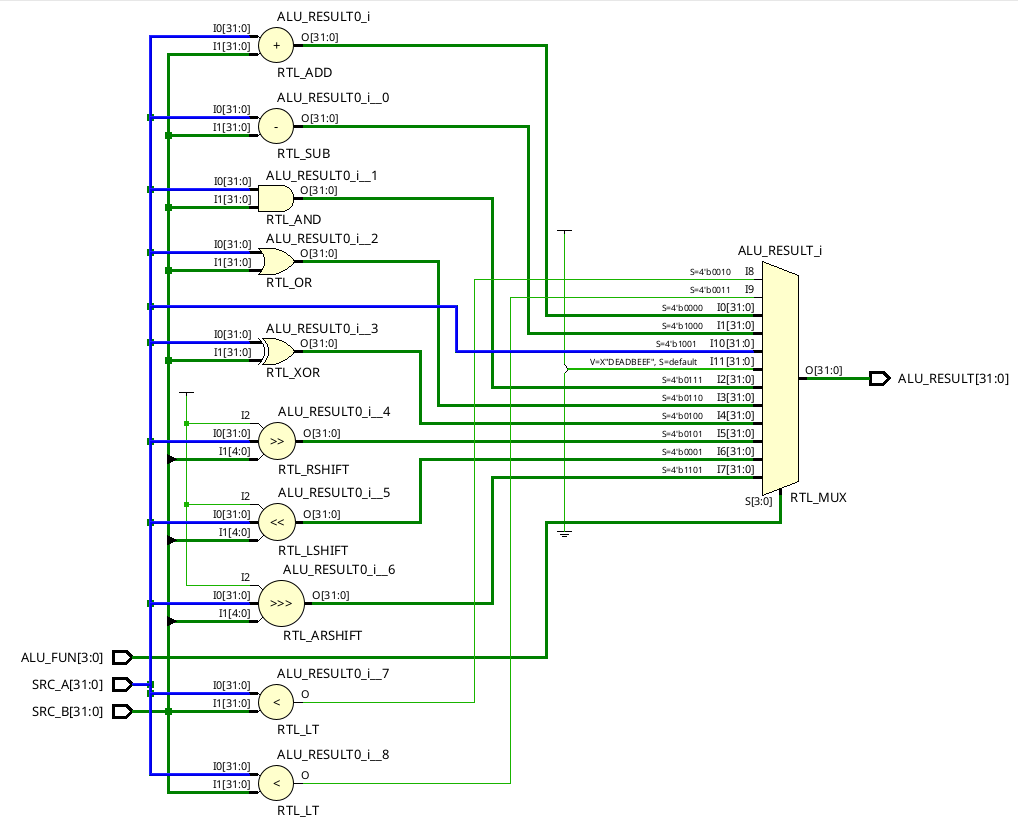
\includegraphics[width=\textwidth]{../03_hardware/hw4/rtl_schematic_alu.png}
					\caption{RTL Design of the ALU}
					\label{fig:-03_hardware-hw4-design_alu-png}
				\end{figure}


				\rowcolors{2}{lightgray!50}{lightgray!50}
				\begin{table}[H]
					\centering
					\begin{tabular}{||c|c|l|l|l||}
						\hline
						\textbf{Function} & \textbf{ALU\_FUN}  & \textbf{Arg A} & \textbf{Arg B} & \textbf{Expected Result} \\\hline
						ADD & 0x0000 & 0xA50F\_96C3  & 0x5AF0\_693C & 0xFFFF\_FFFF  \\\hline
							&  		 & 0x8410\_5F21  & 0x7B10\_5FDE & 0xFF20\_BEFF  \\\hline
							&  		 & 0xFFFF\_FFFF  & 0x0000\_0001 & 0x0000\_0000  \\\hline

						\hiderowcolors
						SUB & 0x1000 & 0x0000\_0000  & 0x0000\_0001 & 0xFFFF\_FFFF  \\\hline
							&  		 & 0xAA80\_6355  & 0x5501\_62AA & 0x557F\_00AB  \\\hline
							&  		 & 0x5501\_62AA  & 0xAA80\_6355 & 0xAA80\_FF55  \\\hline

						\showrowcolors
						AND & 0x0111 & 0xA55A\_00FF  & 0x5A5A\_FFFF & 0x005A\_00FF  \\\hline
							&  		 & 0xC3C3\_F966  & 0xFF66\_9F5A & 0xC342\_9942  \\\hline

						\hiderowcolors
						 OR & 0x0110 & 0x9A9A\_C300  & 0x65A3\_CC0F & 0xFFBB\_CF0F  \\\hline
						 	& 		 & 0xC3C3\_F966  & 0xFF66\_9F5A & 0xFFE7\_FF7E  \\\hline

						\showrowcolors
						XOR & 0x0100 & 0xAA55\_00FF  & 0x5AA5\_0FF0 & 0xF0F0\_0F0F  \\\hline
							& 		 & 0xA5A5\_6C6C  & 0xFF00\_C6FF & 0x5AA5\_AA93  \\\hline

						\hiderowcolors
						SRL & 0x0101 & 0x805A\_6CF3  & 0x0000\_0010 & 0x0000\_805A  \\\hline
							&		 & 0x705A\_6CF3  & 0x0000\_0005 & 0x0382\_D367  \\\hline
							&  		 & 0x805A\_6CF3  & 0x0000\_0000 & 0x805A\_6CF3  \\\hline
							&		 & 0x805A\_6CF3  & 0x0000\_0100 & 0x805A\_6CF3  \\\hline

						\showrowcolors
						SLL & 0x0001 & 0x805A\_6CF3  & 0x0000\_0010 & 0x6CF3\_0000  \\\hline
							&  		 & 0x805A\_6CF3  & 0x0000\_0005 & 0x0B4D\_9E60  \\\hline
							&		 & 0x805A\_6CF3  & 0x0000\_0100 & 0x805A\_6CF3  \\\hline

						\hiderowcolors
						SRA & 0x1101 & 0x805A\_6CF3  & 0x0000\_0010 & 0xFFFF\_805A  \\\hline
							&		 & 0x705A\_6CF3  & 0x0000\_0005 & 0x0382\_D367  \\\hline
							&  		 & 0x805A\_6CF3  & 0x0000\_0000 & 0x805A\_6CF3  \\\hline
							&		 & 0x805A\_6CF3  & 0x0000\_0100 & 0x805A\_6CF3  \\\hline

						\showrowcolors
						SLT & 0x0010 & 0x7FFF\_FFFF  & 0x8000\_0000 & 0x0000\_0000  \\\hline
							&		 & 0x8000\_0000  & 0x0000\_0001 & 0x0000\_0001  \\\hline
							&  		 & 0x0000\_0000  & 0x0000\_0000 & 0x0000\_0000  \\\hline
							&		 & 0x5555\_5555  & 0x5555\_5555 & 0x0000\_0000  \\\hline

						\hiderowcolors
						SLTU& 0x0011 & 0x7FFF\_FFFF  & 0x8000\_0000 & 0x0000\_0001  \\\hline
							&		 & 0x8000\_0000  & 0x0000\_0001 & 0x0000\_0000  \\\hline
							&  		 & 0x0000\_0000  & 0x0000\_0000 & 0x0000\_0000  \\\hline
							&		 & 0x55AA\_55AA  & 0x55AA\_55AA & 0x0000\_0000  \\\hline
					
						\showrowcolors
						LUI COPY (MV?) & 0x1001 & 0x0123\_4567  & 0x7654\_3210 & 0x0123\_4567 \\\hline
							&		 & 0xFEDC\_BA98  & 0x89AB\_CDEF &  0xFEDC\_BA98 \\\hline

						\hiderowcolors
					\end{tabular}
					\label{tab:ALU-verify}
					\caption{ALU Required Test Cases for Verification}
				\end{table}
				
				See \texttt{ALU.sv} \ref{otter:alu} and \texttt{ALU\_tb.sv} \ref{ottertest:alu}
				for passing simulation test cases from table \ref{tab:ALU-verify}.


			\subsubsection{Immediate Generator}
				\begin{figure}[H]
					\centering
					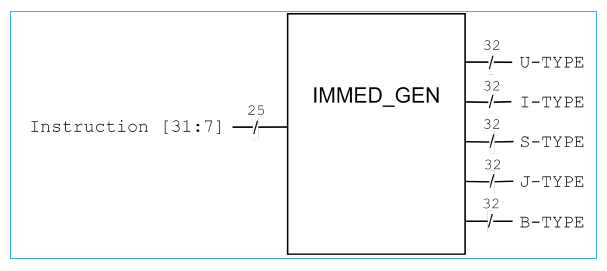
\includegraphics[width=0.5\textwidth]{../03_hardware/hw4/target_immed.png}
					\caption{Top Level ImmedGen}
					\label{fig:-03_hardware-hw4-target_gen-png}
				\end{figure}

				The Immediate Generator is a feed though bit parser for
				different assembly instructions, continuously outputting
				all types per instruction.

				\begin{figure}[H]
					\centering
					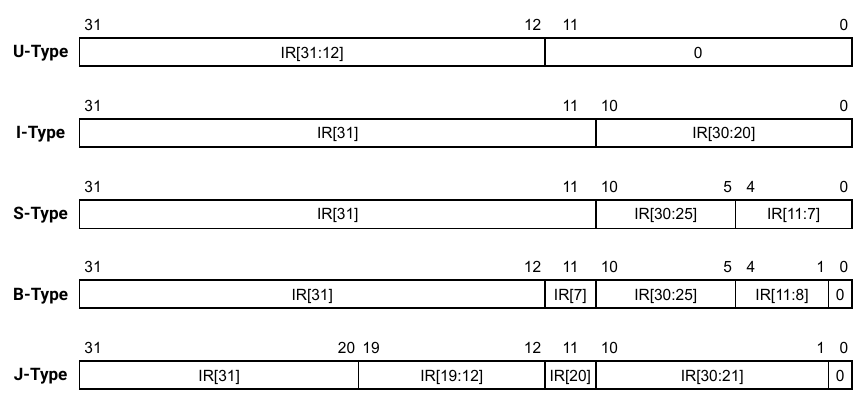
\includegraphics[width=0.8\textwidth]{../03_hardware/hw4/design_immed.png}
					\caption{Instruction types of the Immediate Generator}
					\label{fig:-03_hardware-hw4-design_immed-png}
				\end{figure}

				\begin{figure}[H]
					\centering
					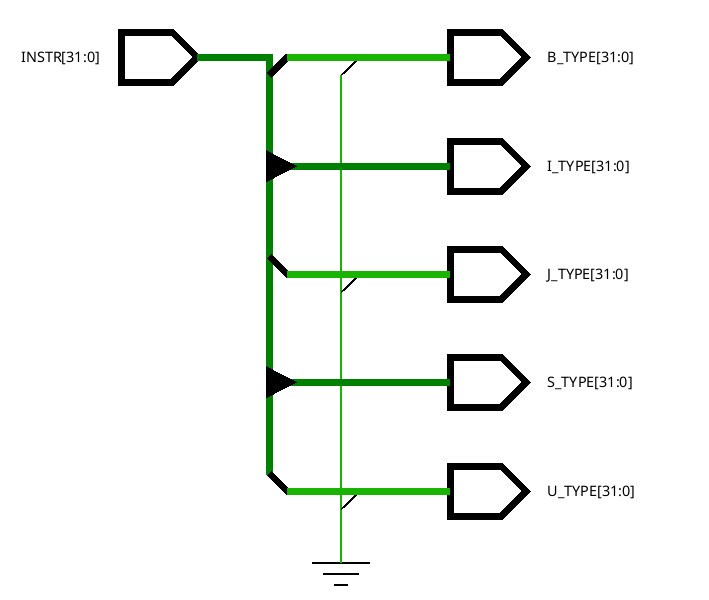
\includegraphics[width=0.6\textwidth]{../03_hardware/hw4/rtl_schematic_immed.png}
					\caption{RTL Design of the ImmedGen}
					\label{fig:-03_hardware-hw4-design_immed-png}
				\end{figure}

				See \texttt{ImmedGen.sv} \ref{otter:immgen} and \texttt{ImmedGen\_tb.sv} 
				\ref{ottertest:immgen} for passing simulation test cases

		\newpage
		\subsection{HW5 - Real Memory and Branch}

			\subsubsection{Memory}

				The memory segment is designed to dual synch output an instruction
				and a data value with architecture for pulling data from the 
				MMIO addresses. They are on separate addresses physically 
				such that they are not on the stack but rather beyond 
				what could be the heap (if we implement one). 

				\begin{figure}[H]
					\centering
					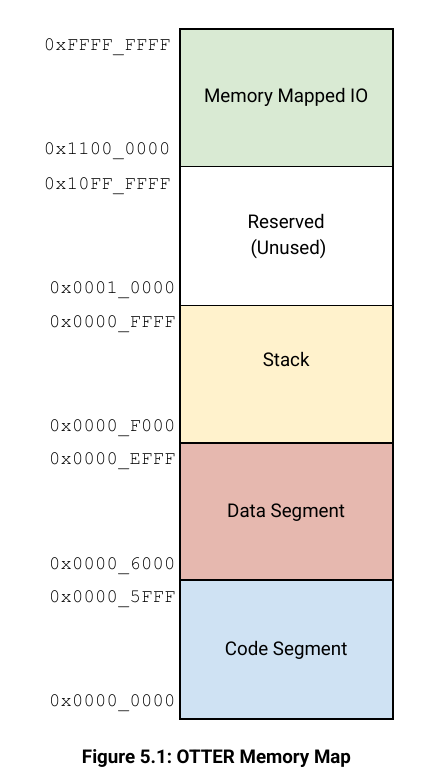
\includegraphics[width=0.3\textwidth]{../03_hardware/hw5/mem_map.png}
					\caption{Memory Map for OTTER}
					\label{fig:-03_hardware-hw5-mem-map-png}
				\end{figure}

				\begin{figure}[H]
					\centering
					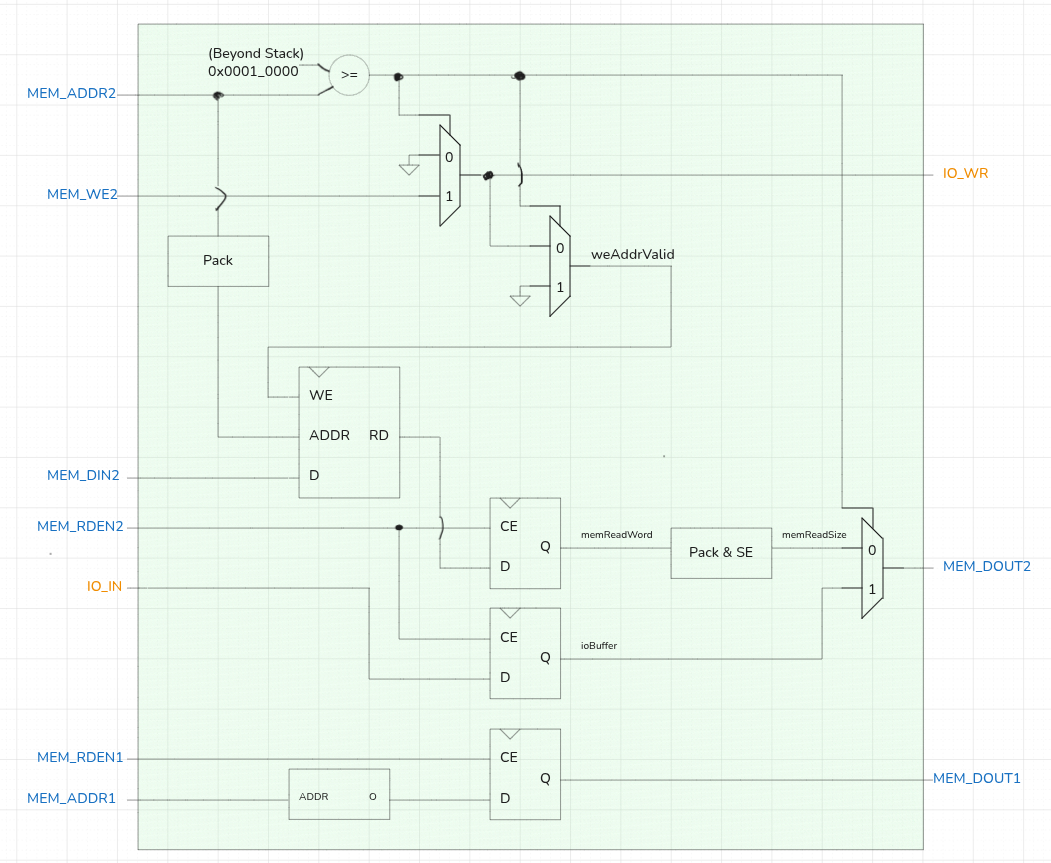
\includegraphics[width=\textwidth]{../03_hardware/hw5/mem_flow.png}
					\caption{\textbf{ROUGH} Flow Diagram for Memory}
					\label{fig:-03_hardware-hw5-memory_flow-png}
				\end{figure}

				\rowcolors{2}{white!50}{lightgray!50}
				\begin{table}[H]
					\centering
					\label{tab:memory}
					\begin{tabular}{|l|c|c|}
						\hline
						\textbf{Signal} & \textbf{Size(bits)} & \textbf{Purpose} \\ \hline
						\showrowcolors
						MEM\_CLK	& 1		& Required for synchronous logic \\\hline
						MEM\_RDEN1	& 1		& Request an instr read at ADDR1, to register, to DOUT1 \\\hline
						MEM\_RDEN2	& 1 	& Request a value read at ADDR2 with path to update DOUT2 (but not entire path)\\\hline
						MEM\_WE2	& 1		& Request DIN2 overwrite register connected to DOUT | wire to IO\_WR \\\hline
						MEM\_ADDR1	& 14	& Instruction address \\\hline
						MEM\_ADDR2	& 32	& Data Address \\\hline
						MEM\_DIN2	& 32	& Data value to overwrite one at ADDR2\\\hline
						MEM\_SIZE	& 2		& Indicate (Byte, Half, Word) size of data going to ADDR2\\\hline
						MEM\_SIGN	& 1		& Indicate (signed, unsigned) data going to ADDR2\\\hline
						IO\_IN		& 32	& Incoming data from IO\\\hline
						IO\_WR		& 1		& Feedthrough of MEM\_WE2 if ADDR2 is in MMIO range\\\hline
						MEM\_DOUT1	& 32	& Instr1 output \\\hline
						MEM\_DOUT2	& 32	& Data2 output \\\hline
					\end{tabular}
					\caption{Memory Module Signals}
				\end{table}

				\begin{figure}[H]
					\centering
					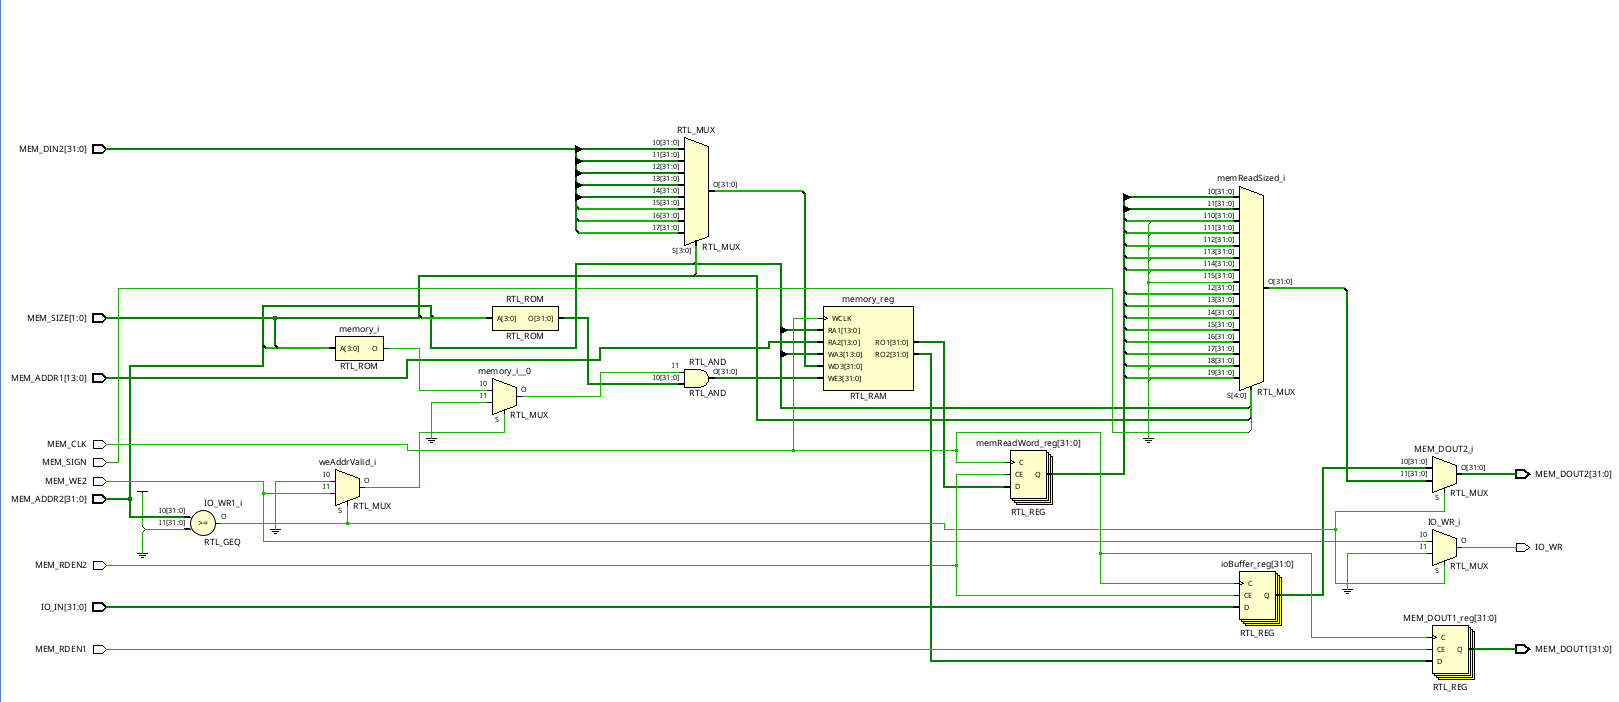
\includegraphics[width=\textwidth]{../03_hardware/hw5/rtl_schematic_mem.png}
					\caption{Lint RTL Schematic of Memory}
					\label{fig:-03_hardware-hw5-rtl_mem-png}
				\end{figure}

				See \texttt{otter\_memory\_v1\_07.sv} \ref{otter:memory}.

			\subsubsection{Branch Condition Generator}
		
				The BCG compares two register values and generates a command
				signal for equality, less than (signed), and less than (unsigned).
				This is needed to perform the logic evaluations of the differing
				branch types s.a. beq, bltu, \ldots

				\begin{figure}[H]
					\centering
					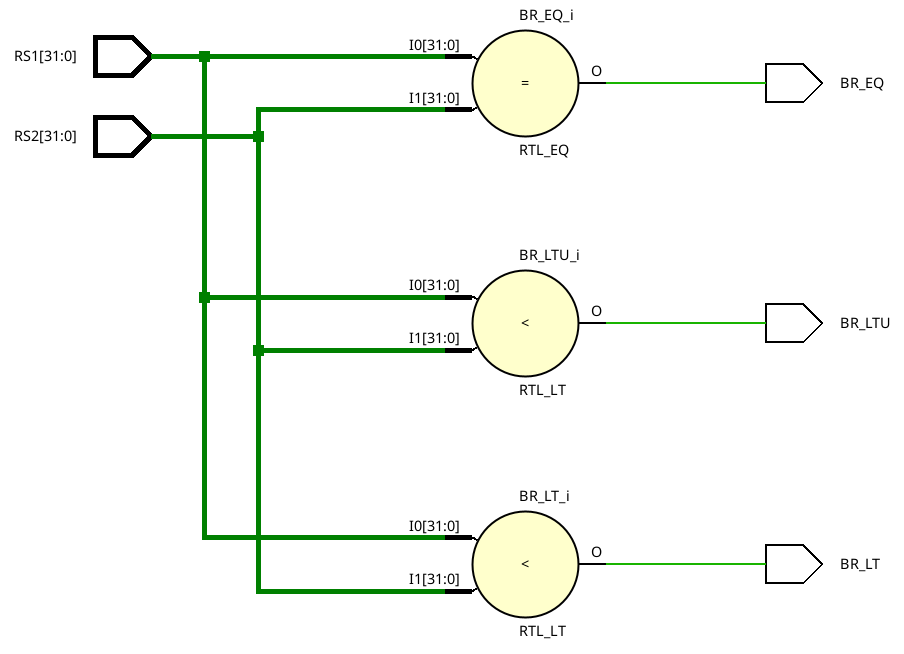
\includegraphics[width=0.6\textwidth]{../03_hardware/hw5/rtl_schematic_BCG.png}
					\caption{Lint RTL Schematic of BCG}
					\label{fig:-03_hardware-hw5-rtl_bcg-png}
				\end{figure}

				See \texttt{BranchConditionGen.sv}\ref{otter:bcondgen} 
				and sim test \texttt{BranchConditionGen\_tb.sv} \ref{ottertest:bcondgen}. 
	
			\subsubsection{Branch Address Generator}
		
				The BAG is used to modify the program counter! We want
				this module s.t. we can jump (J-Type), branch (B-Type), 
				and jump-return (using I-Type). These instructions are
				useful for control flow. 

				\begin{figure}[H]
					\centering
					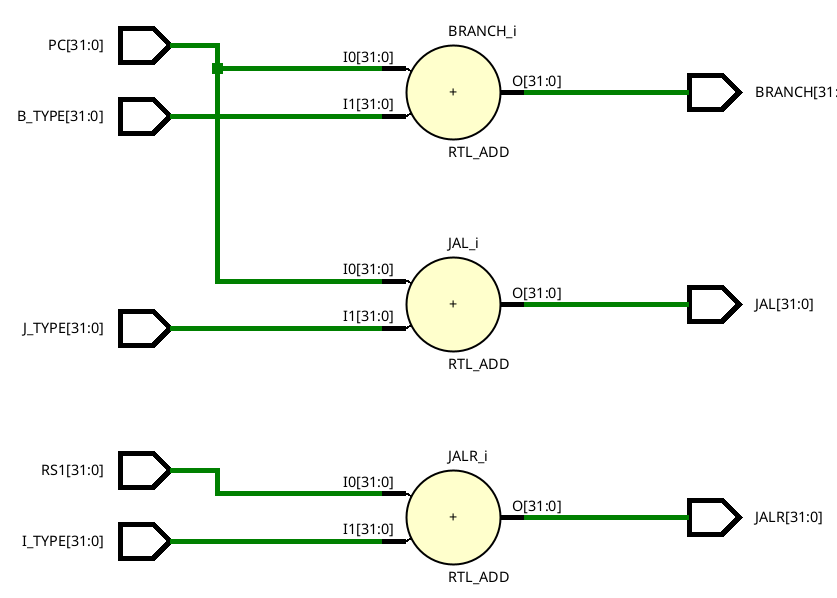
\includegraphics[width=0.6\textwidth]{../03_hardware/hw5/rtl_schematic_BAG.png}
					\caption{Lint RTL Schematic of BAG}
					\label{fig:-03_hardware-hw5-rtl_bag-png}
				\end{figure}

				See \texttt{BranchAddrGen.sv}\ref{otter:baddrgen} 
				and sim test \texttt{BranchAddrGen\_tb.sv} \ref{ottertest:baddrgen}. 

		\newpage
		\subsection{HW6 - Control Unit}

			\begin{figure}[H]
				\centering
				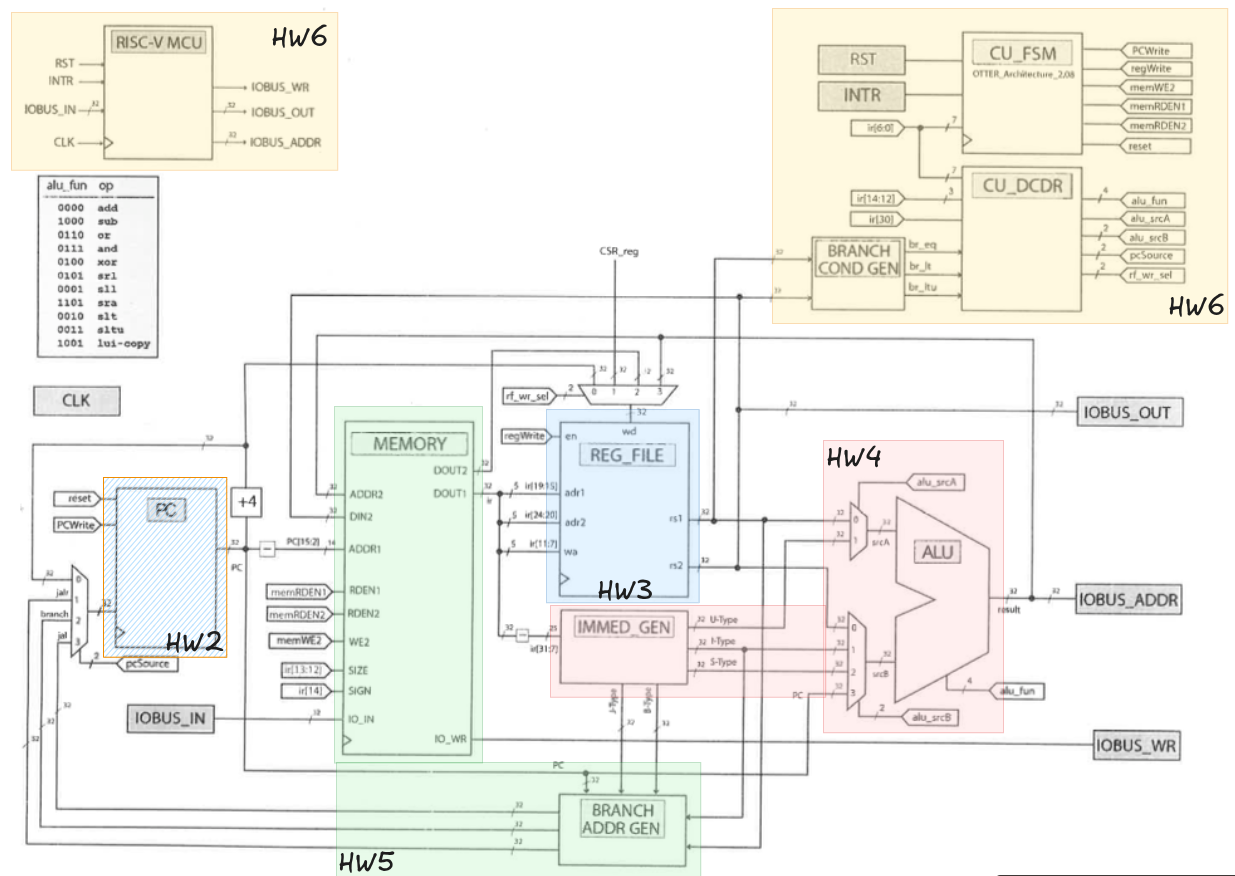
\includegraphics[width=0.8\textwidth]{../03_hardware/hw6/so_far.png}
				\caption{MultiCycle Otter after HW6}
				\label{fig:w6otter}
			\end{figure}

			Data and control mapping is different for each type of instruction.
			Therefore, I've provided the various configurations per instruction
			type below. 

			\begin{figure}[H]
				\centering
				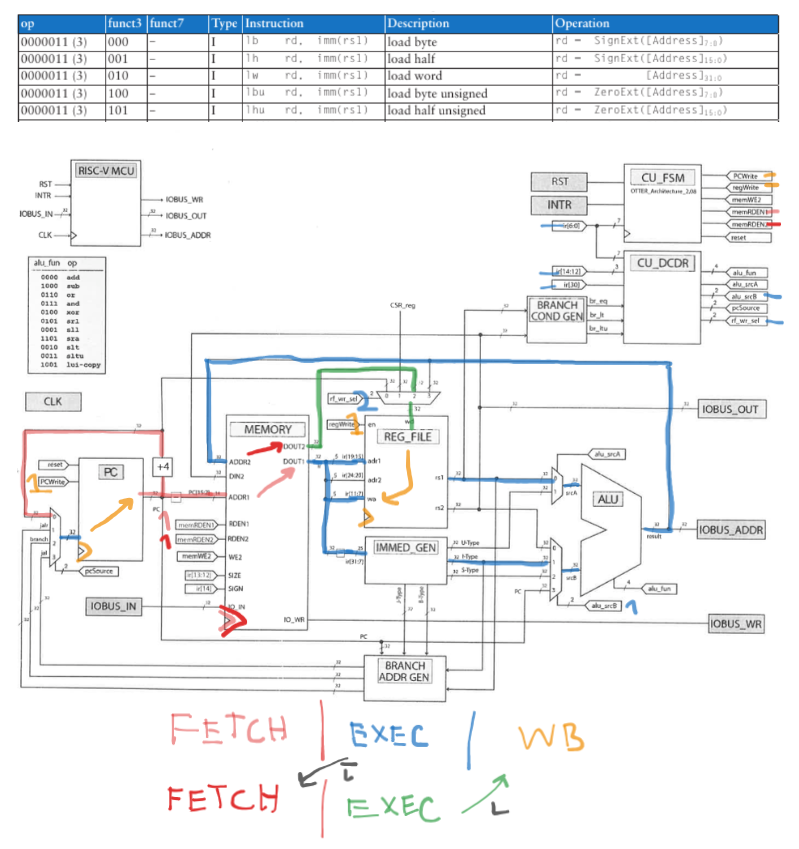
\includegraphics[width=0.8\textwidth]{../03_hardware/hw6/d1.png}
				\caption{MultiCycle Otter Pathing for \texttt{load}}
				\label{fig:map-load}
			\end{figure}

			\begin{figure}[H]
				\centering
				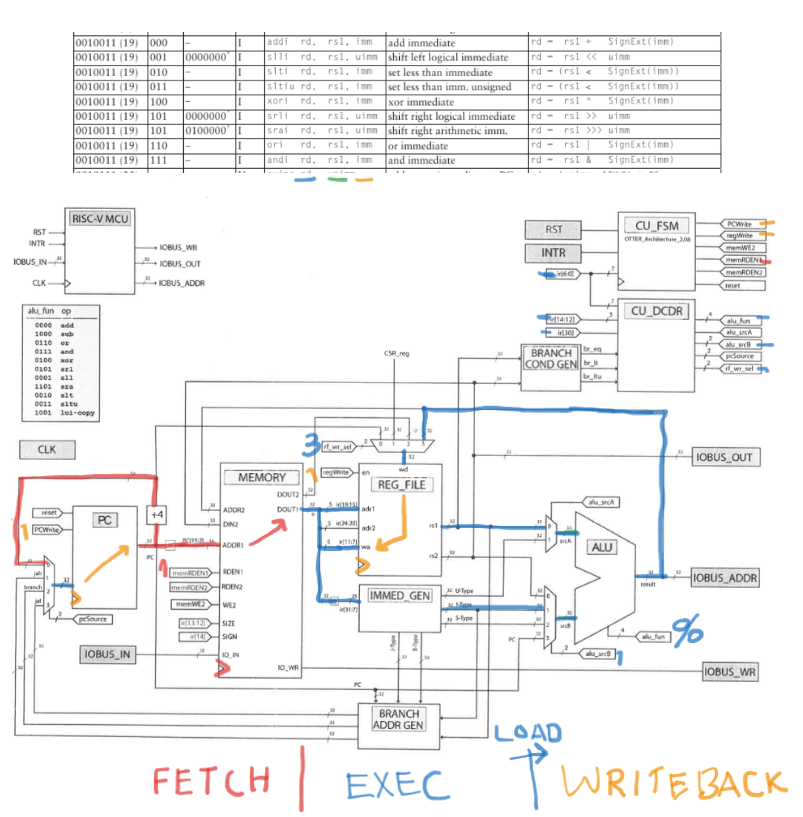
\includegraphics[width=0.8\textwidth]{../03_hardware/hw6/d2.png}
				\caption{MultiCycle Otter Pathing for \texttt{immed ops}}
				\label{fig:map-immed}
			\end{figure}

			\begin{figure}[H]
				\centering
				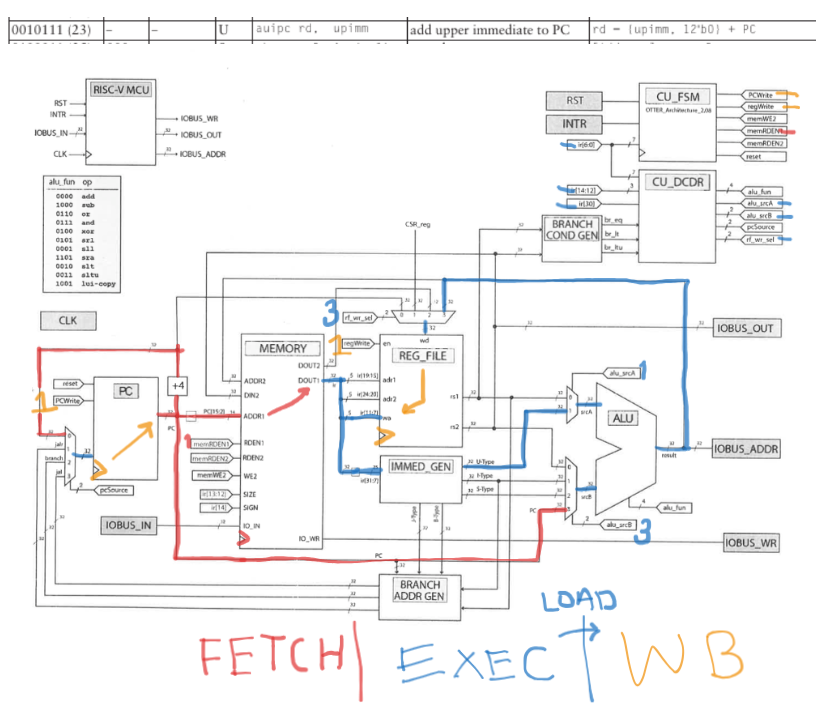
\includegraphics[width=0.8\textwidth]{../03_hardware/hw6/d3.png}
				\caption{MultiCycle Otter Pathing for \texttt{auipc}}
				\label{fig:map-auipc}
			\end{figure}

			\begin{figure}[H]
				\centering
				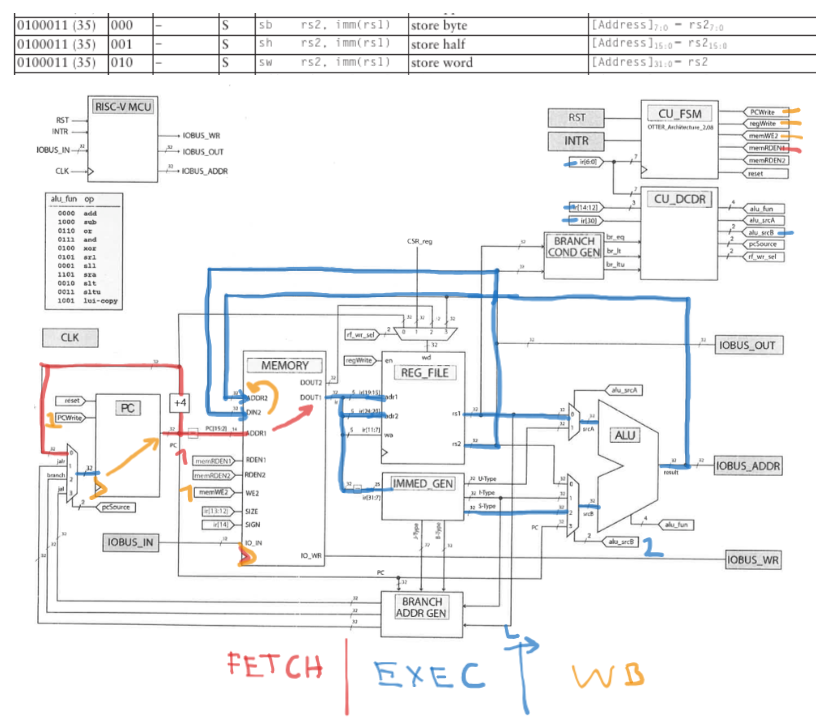
\includegraphics[width=0.8\textwidth]{../03_hardware/hw6/d4.png}
				\caption{MultiCycle Otter Pathing for \texttt{store}}
				\label{fig:map-store}
			\end{figure}

			\begin{figure}[H]
				\centering
				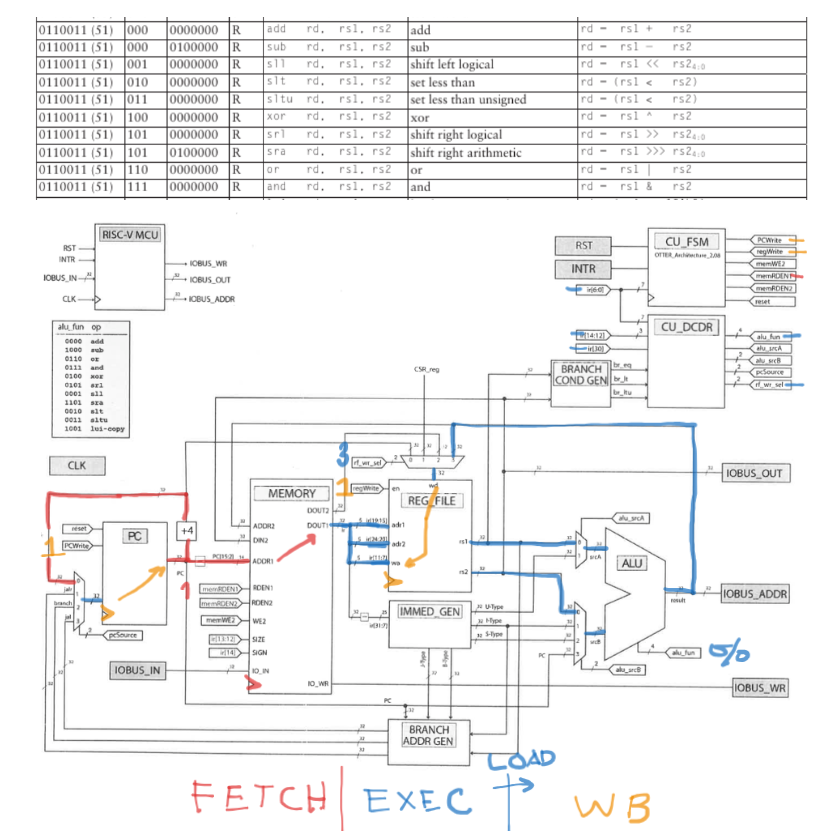
\includegraphics[width=0.8\textwidth]{../03_hardware/hw6/d5.png}
				\caption{MultiCycle Otter Pathing for \texttt{dual register ops}}
				\label{fig:map-dual}
			\end{figure}

			\begin{figure}[H]
				\centering
				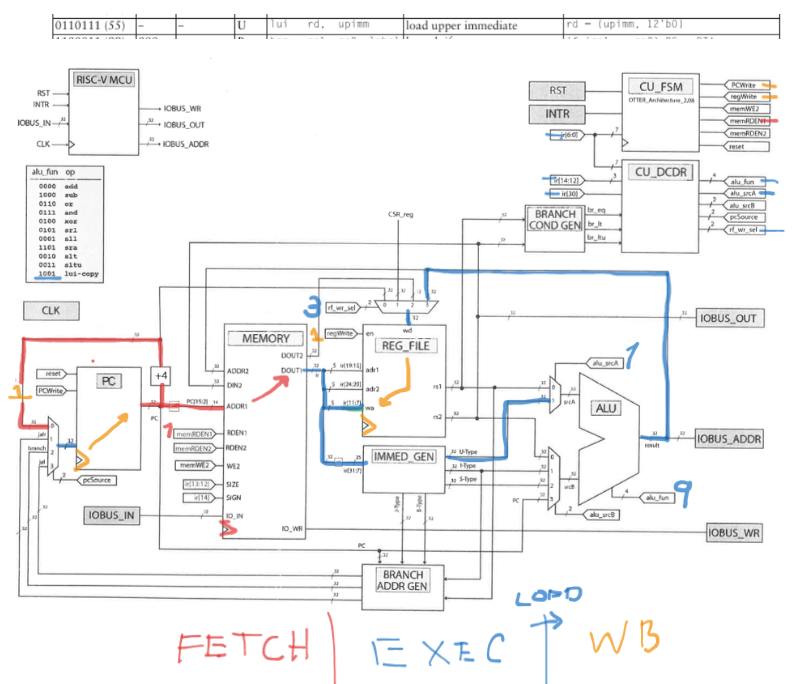
\includegraphics[width=0.8\textwidth]{../03_hardware/hw6/d6.png}
				\caption{MultiCycle Otter Pathing for \texttt{lui}}
				\label{fig:map-lui}
			\end{figure}

			\begin{figure}[H]
				\centering
				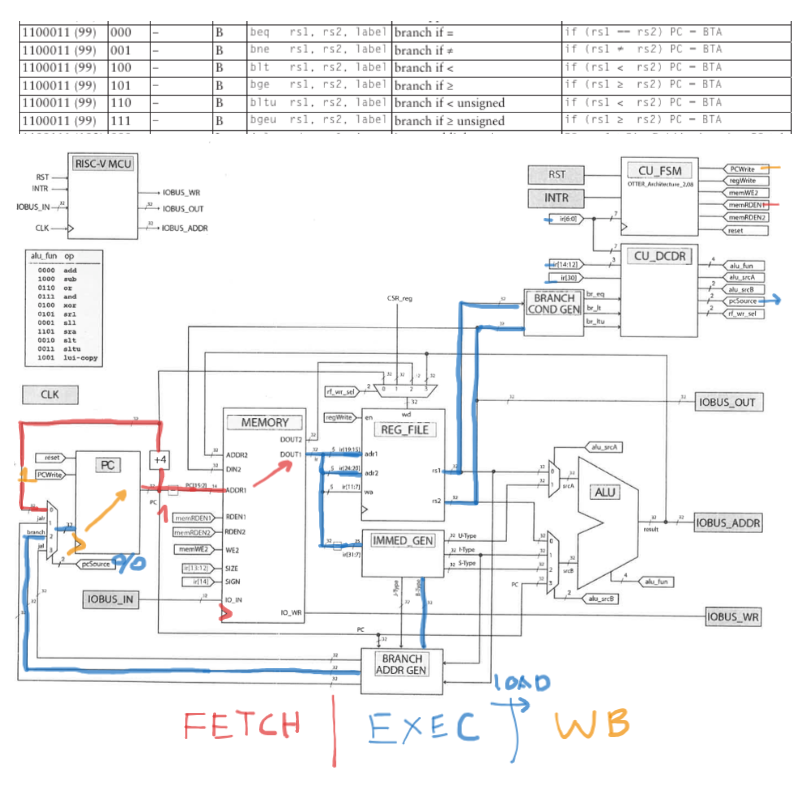
\includegraphics[width=0.8\textwidth]{../03_hardware/hw6/d7.png}
				\caption{MultiCycle Otter Pathing for \texttt{branch}}
				\label{fig:map-branch}
			\end{figure}

			\begin{figure}[H]
				\centering
				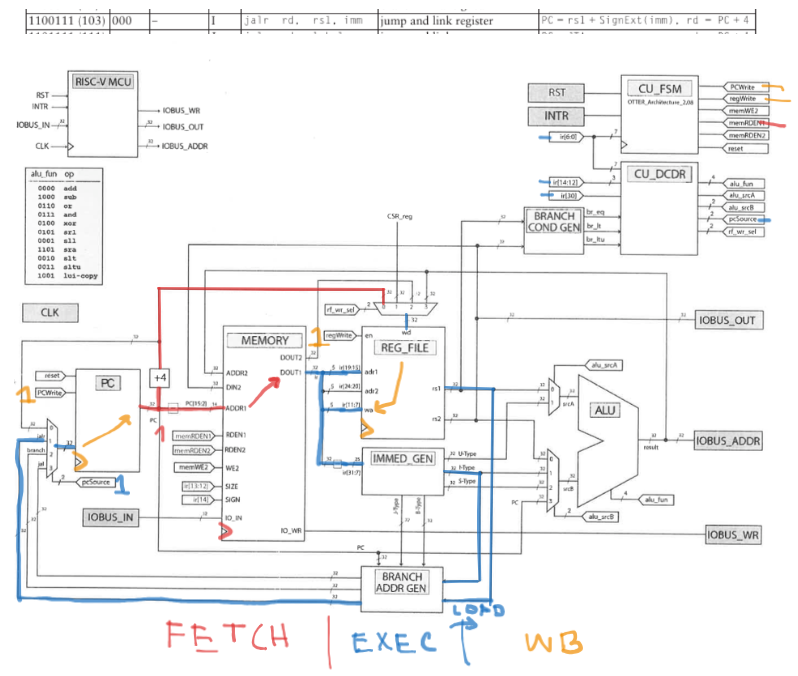
\includegraphics[width=0.8\textwidth]{../03_hardware/hw6/d8.png}
				\caption{MultiCycle Otter Pathing for \texttt{jalr}}
				\label{fig:map-jalr}
			\end{figure}

			\begin{figure}[H]
				\centering
				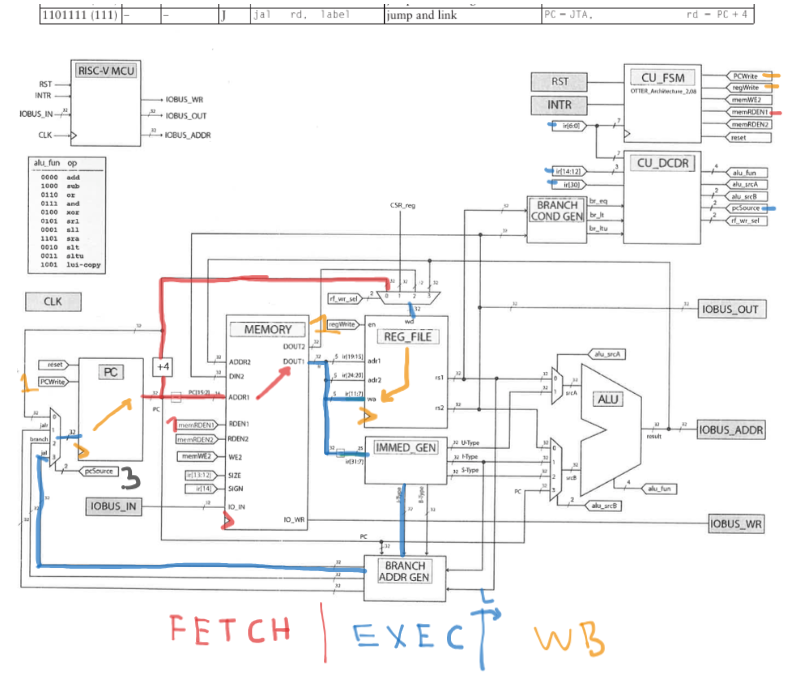
\includegraphics[width=0.8\textwidth]{../03_hardware/hw6/d9.png}
				\caption{MultiCycle Otter Pathing for \texttt{jal}}
				\label{fig:map-jal}
			\end{figure}

			\subsubsection{Control Unit Decoder}

				After mapping the data and control signals, we need a way
				to control data flowing into the ALU, register file, program
				counter, as well as the ALU itself. We depend on the Decoder
				to do this, writing to the selectors for each mux. Note
				that the decoder can only make an intelligent switch during
				and after the EXEC cycle s.t. the opcode is available to process. 

				\begin{figure}[H]
					\centering
					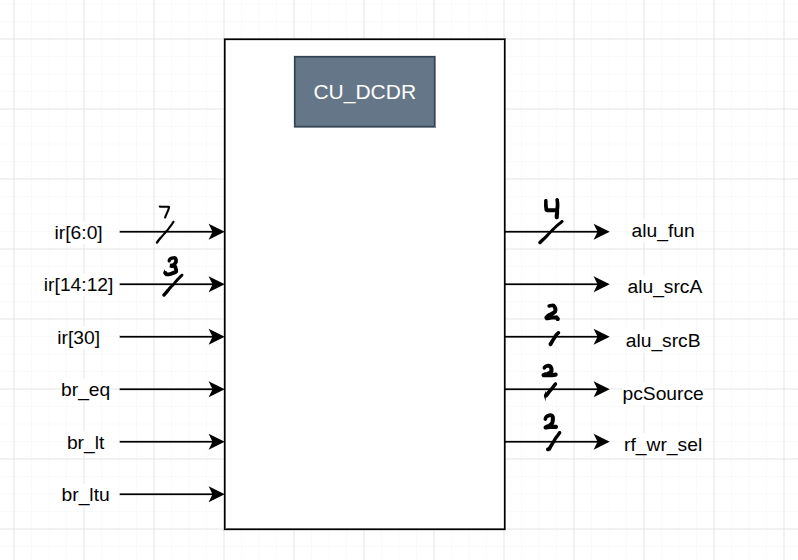
\includegraphics[width=0.8\textwidth]{../03_hardware/hw6/decoder_module.png}
					\caption{Control Unit Decoder Top Level}
					\label{fig:hw6-decoder-module}
				\end{figure}

				\begin{figure}[H]
					\centering
					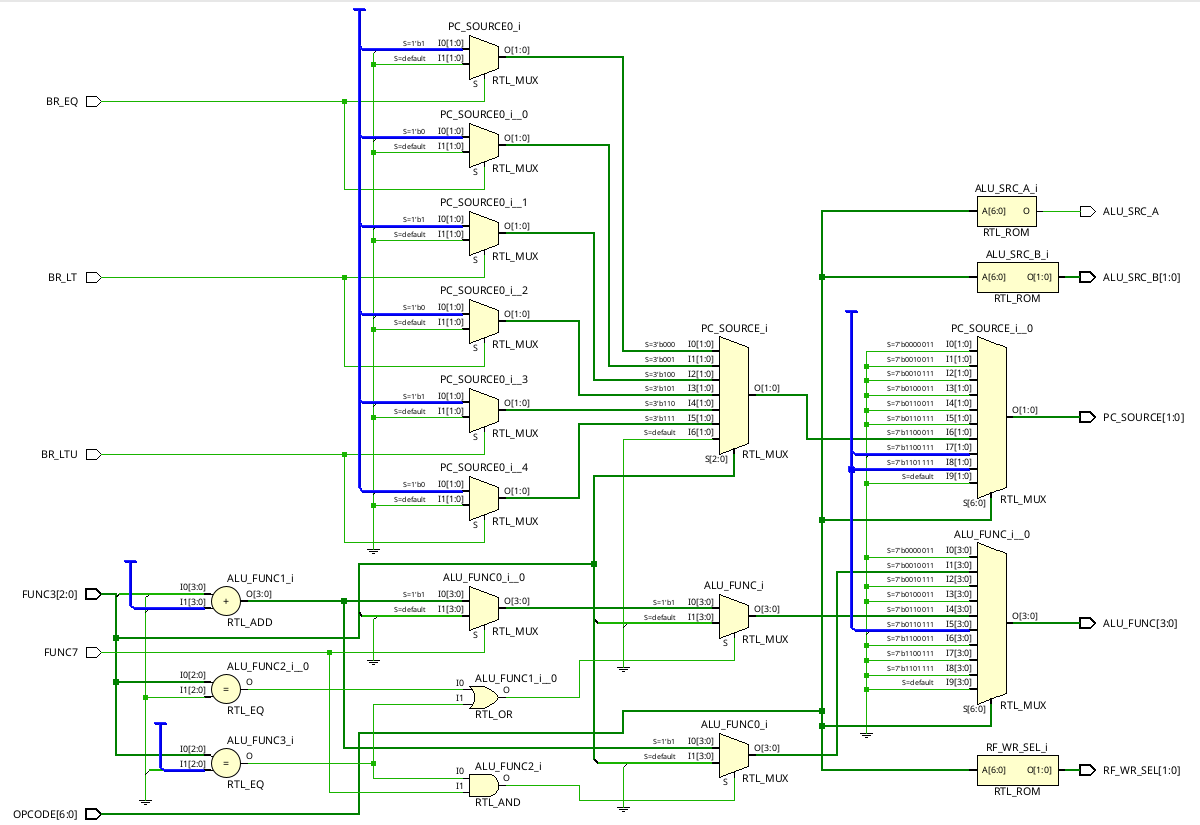
\includegraphics[width=0.8\textwidth]{../03_hardware/hw6/decoder_rtl.png}
					\caption{Control Unit Decoder RTL}
					\label{fig:hw6-decoder-rtl}
				\end{figure}

				See \texttt{CUnit\_Decoder.sv} \ref{otter:cudecoder} and 
				sim test cases \texttt{CUnit\_Decoder\_tb.sv} \ref{ottertest:cudecoder}.

			\subsubsection{Control Unit FSM}

				With the decoder controlling the data/mux selectors, we need
				a module to issue the control signals for read/writing. 
				The FSM allows us to do just that, toggling read signals
				for memory and PC while also controlling when to write
				contents in memory and registers. We've confined our FSM
				to 4 stages (INIT, FETCH, EXEC, WRITEBACK). 

				\begin{figure}[H]
					\centering
					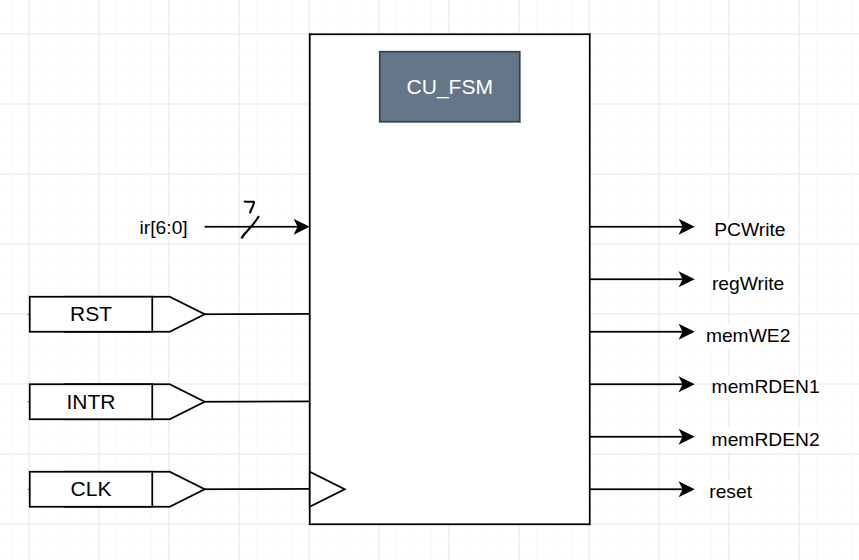
\includegraphics[width=0.8\textwidth]{../03_hardware/hw6/fsm_module.png}
					\caption{Control Unit FSM Top Level}
					\label{fig:hw6-fsm-module}
				\end{figure}

				\begin{figure}[H]
					\centering
					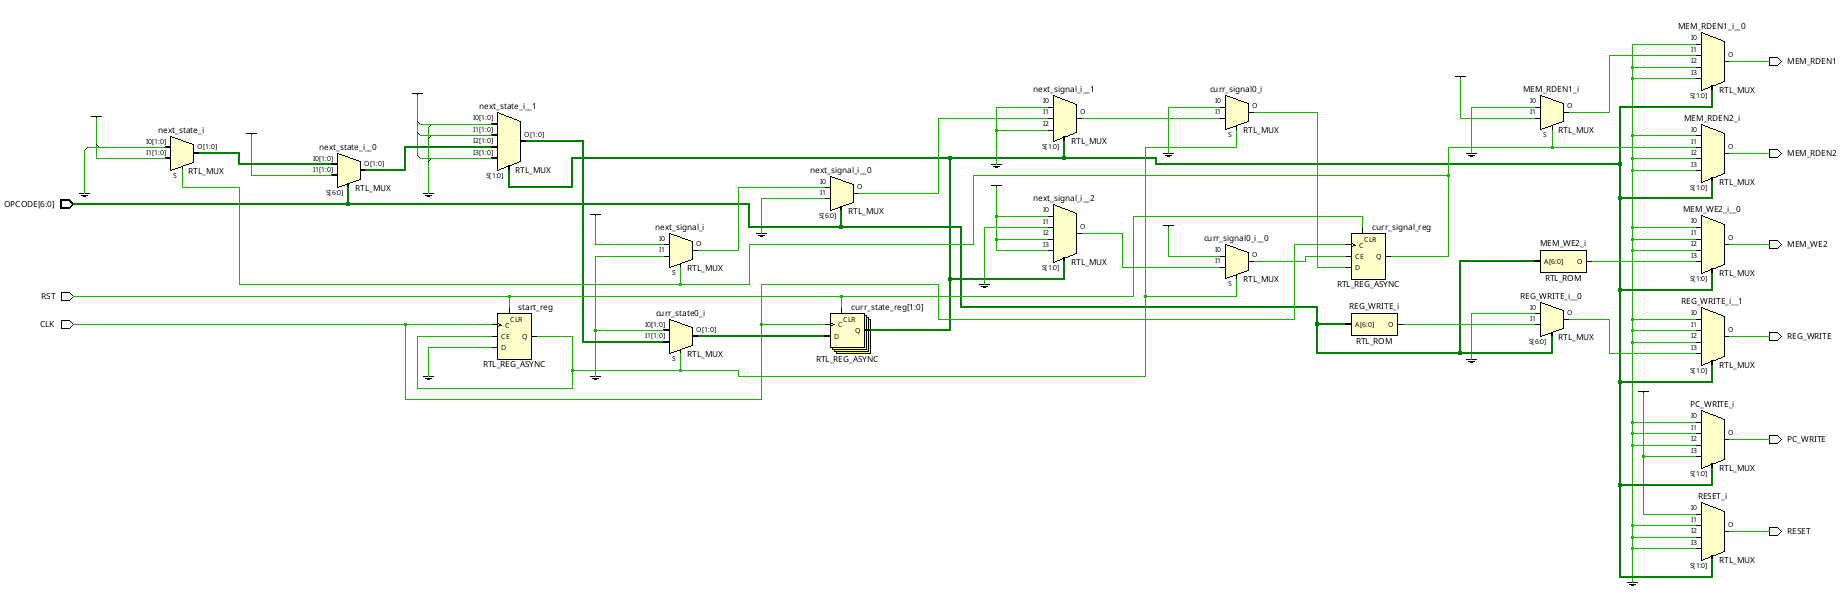
\includegraphics[width=\textwidth]{../03_hardware/hw6/fsm_rtl.png}
					\caption{Control Unit FSM RTL}
					\label{fig:hw6-fsm-rtl}
				\end{figure}

				\textbf{Stages} :
				\begin{itemize}
					\item \textbf{INIT} : stage upon startup or reset that
							zeros out all signals.

					\item \textbf{FETCH} : PC is available and this stage
							processes the contents at that PC address, tucked away 
							inside the memory module. By the end, DOUT1 should be 
							available (and maybe DOUT2 depending on the instr).

					\item \textbf{EXEC} : stage is used to give instr operations
							runway to compute and arrive to their respective mux channels.

					\item \textbf{WRITEBACK} : stage is used to overwrite a 
							desired PC, memory, or register.
							
				\end{itemize}

				\begin{figure}[H]
					\centering
					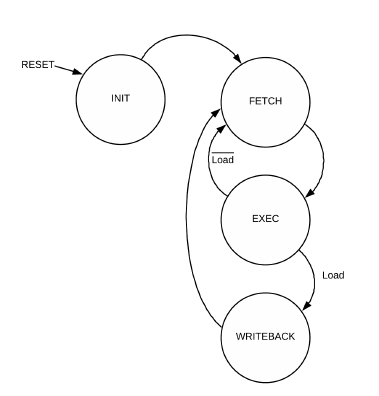
\includegraphics[width=0.6\textwidth]{../03_hardware/hw6/state_diagram.png}
					\caption{FSM Diagram}
					\label{fig:hw6-state_diagram-png}
				\end{figure}

				See \texttt{CUnit\_FSM.sv} \ref{otter:cufsm} and 
				sim test cases \texttt{CUnit\_FSM\_tb.sv} \ref{ottertest:cufsm}.


			\subsubsection{Otter Micro-Controller}

				At last, we've reached a point where we can combine all created modules
				from HW2-6 and begin to process memory files with RISCV instructions. 

				\begin{figure}[H]
					\centering
					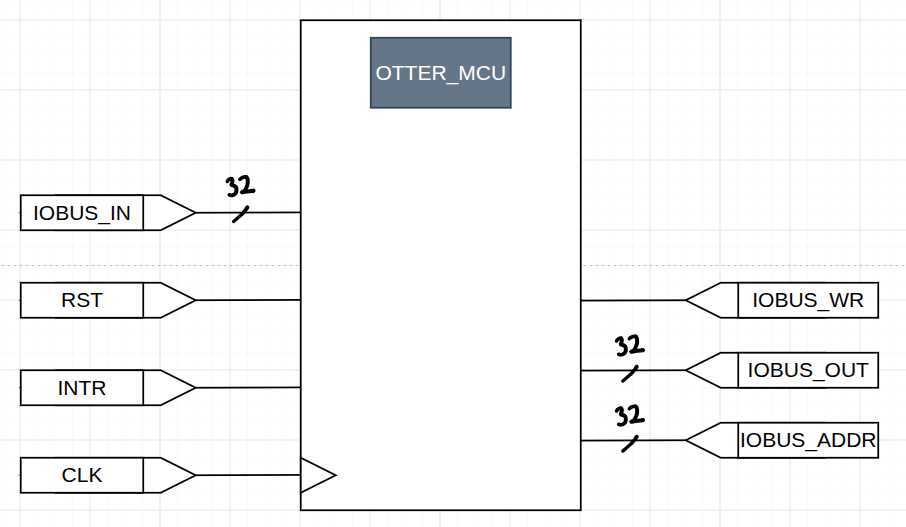
\includegraphics[width=0.8\textwidth]{../03_hardware/hw6/mcu_module.png}
					\caption{OTTER MCU : Non-Interrupt}
					\label{fig:hw6-mcu-module}
				\end{figure}

				\begin{figure}[H]
					\centering
					\includegraphics[width=\textwidth]{../03_hardware/hw6/mcu_schematic_export.pdf}
					\caption{MCU RTL}
					\label{fig:hw6-mcu-rtl}
				\end{figure}

				\begin{figure}[H]
					\centering
					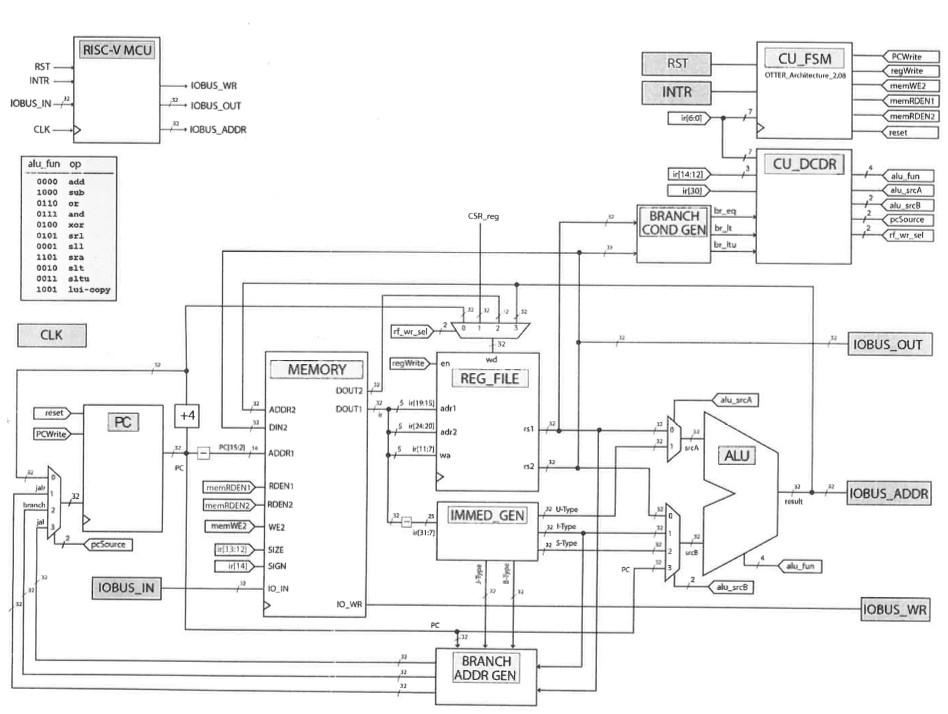
\includegraphics[width=0.8\textwidth]{../OTTER_arch_multicycle_noCSR.png}
					\caption{Non-Interrupt MultiCycle RISCV Otter}
					\label{fig:no-interr-otter}
				\end{figure}

				To perform a small validation for the MCU, a small assembly file
				was created, compiled under RARS tool for RISCV compatibility, 
				and the memory dump (\texttt{otter\_hw6sample\_test.mem}) injected 
				into the memory portion of the OTTER MCU Memory. 

				\lstinputlisting[
					language={[riscv]Assembler},
					captionpos=top,
					caption={Simple Test Script},
					breaklines=false]
				{../03_hardware/hw6/demo.asm}

				\begin{figure}[H]
					\centering
					\includegraphics[width=0.5\textwidth]{../03_hardware/hw6/memconfig.png}
					\caption{Memory config for RARS}
				\end{figure}

				\begin{figure}[H]
					\centering
					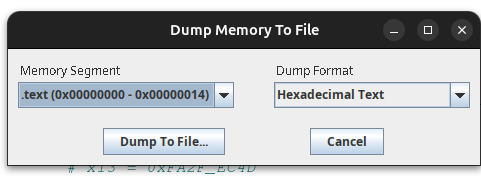
\includegraphics[width=0.5\textwidth]{../03_hardware/hw6/dumpconfig.png}
					\caption{Memory dump config for RARS}
				\end{figure}

				\begin{figure}[H]
					\centering
					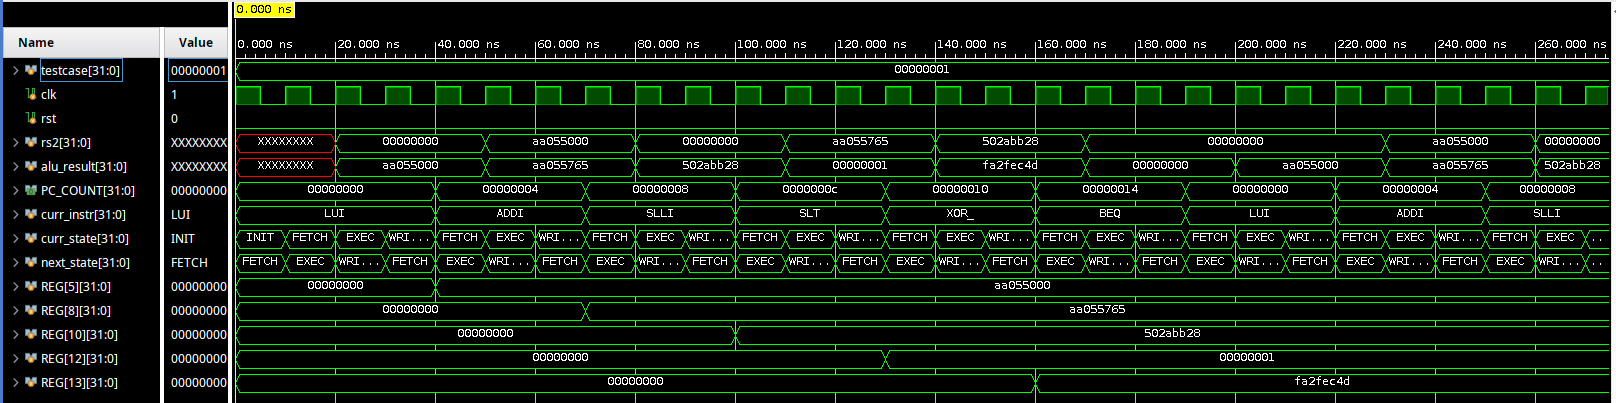
\includegraphics[width=\textwidth]{../03_hardware/hw6/sampletest_waveform.png}
					\caption{Verification Waveforms in simulation testing}
				\end{figure}


				See \texttt{Otter\_MCU.sv} \ref{otter:mcu} and 
				sim test cases \texttt{Otter\_MCU\_tb.sv} \ref{ottertest:mcu}.

		\newpage
		\subsection{HW7 - Otter Wrapper}

			The Otter Wrapper expanded the MCU I/O BUS capabilities to accept
			the onboard switches as input as well as LED/7SEG as outputs (as
			defined in the constraints file \ref{otter:constraint}). In integrating 
			the new peripherals, we've injected a testall memory dump \texttt{diego\_Test\_All.mem} 
			that ideally exercises all RISCV-I instructions and displays the results
			on actual hardware, giving a visual inspection of the hardware 
			as well as the internals. All of these tests passed accordingly. 

			\begin{figure}[H]
				\centering
				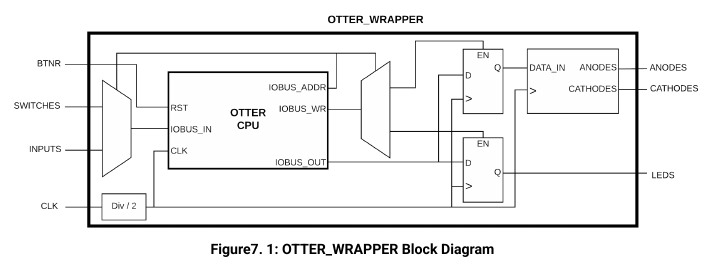
\includegraphics[width=\textwidth]{../03_hardware/hw7/wrapper_schematic.png}
				\caption{Otter Wrapper Schematic}
			\end{figure}

			\begin{figure}[H]
				\centering
				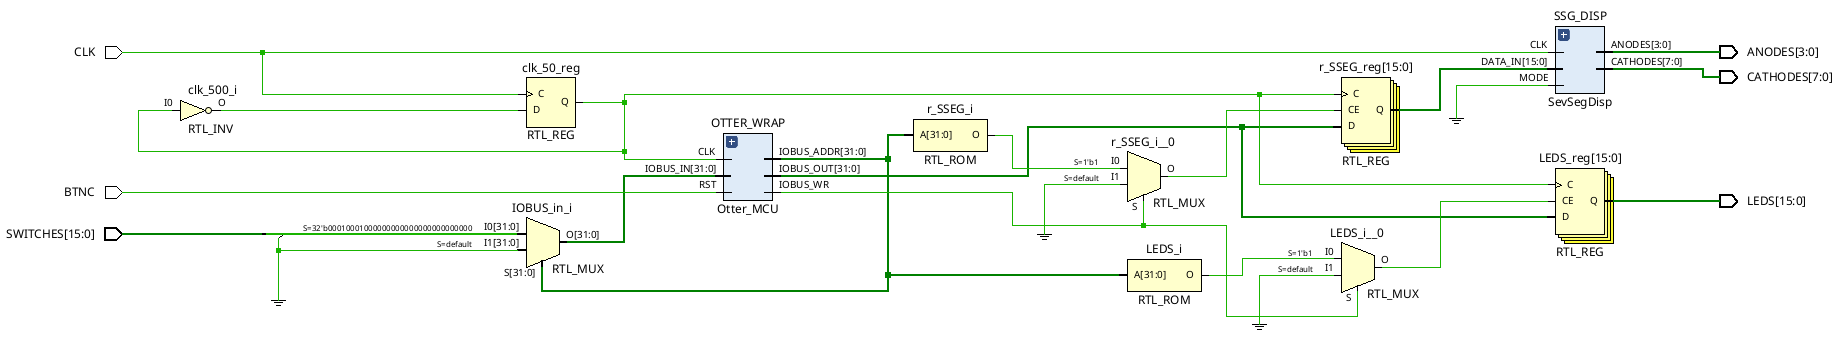
\includegraphics[width=\textwidth]{../03_hardware/hw7/wrapper_rtl.png}
				\caption{Otter Wrapper RTL}
			\end{figure}

			See \ref{otter:wrap} and \ref{ottertest:wrap} for wrapper code and test
			sim. 
			

		\newpage
		\subsection{HW8 - Interrupts}

			\begin{figure}[H]
				\centering
				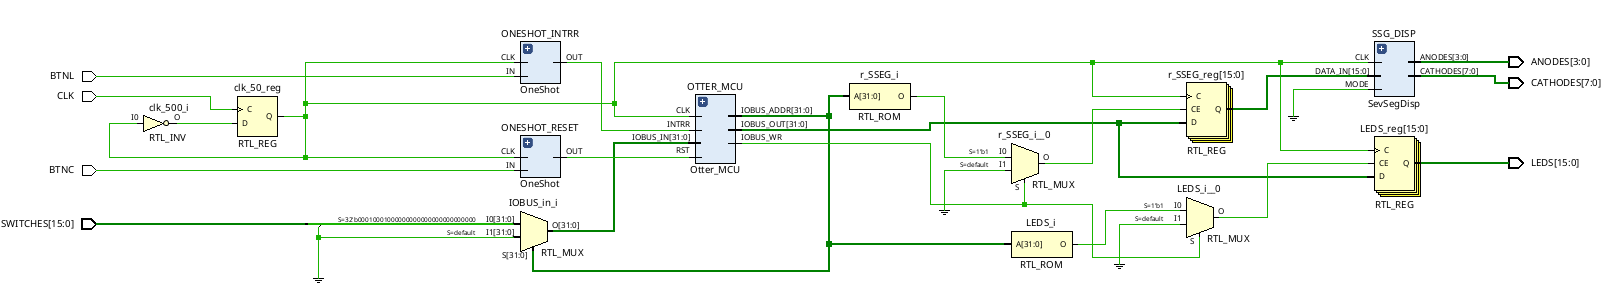
\includegraphics[width=\textwidth]{../03_hardware/hw8/rtl_wrapper.png}
				\caption{Otter Wrapper RTL w/ Interrupts Enabled}
			\end{figure}

			\begin{figure}[H]
				\centering
				\includegraphics[width=\textwidth]{../OTTER_arch_multicycle_CSR.pdf}
				\caption{Schematic of Otter MCU w/ Interrupts Enabled}
			\end{figure}

			\newpage
			\begin{figure}[H]
				\centering
				\includegraphics[
					angle=90,
					origin=c,
					trim= 5mm 90mm 5mm 90mm,
					clip,
					width=0.4\paperheight,
					%height=\paperwidth	
					keepaspectratio=true
				]{../03_hardware/hw8/rtl_mcu.pdf}
				\caption{Otter Wrapper RTL w/ Interrupts Enabled}
			\end{figure}
			\newpage

			\begin{figure}[H]
				\centering
				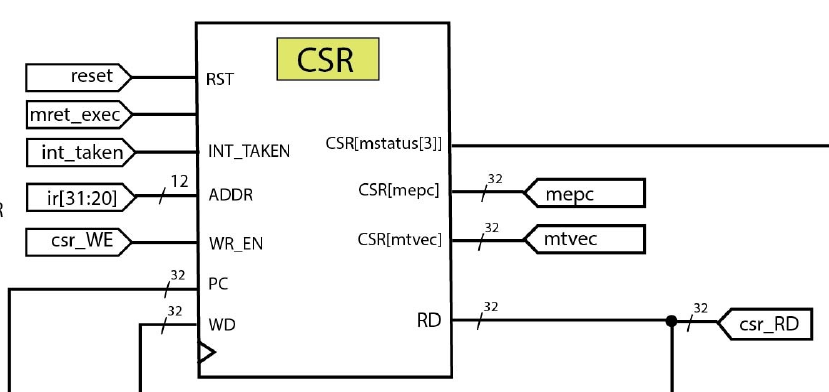
\includegraphics[width=0.7\textwidth]{../03_hardware/hw8/csr_block.png}
				\caption{Otter's Control Status Register}
			\end{figure}

			The Control Status Register (CSR) is a register file that
			enables Interrupts and other service routines. In our sparse use,
			we use one register, the MTVEC, to store and load the address to 
			our single ISR location. We use another register, the MEPC, 
			to temporarily store and load the PC when entering and exiting 
			an ISR. Lastly, we use a register, the MSTATUS, to store the interrupt
			enable setting as well as prevent other interrupt calls during an 
			interrupt routine. It should be noted that there are write and 
			read calls for the 12-bit registers stored in the CSR but we're 
			only using three (as mentioned above). The CSR stores and loads the 
			registers mentioned above on HIGH activation of signals \texttt{int\_taken}
			and \texttt{mret\_exec} which are generated by the Control Unit FSM. 

			\begin{figure}[H]
				\centering
				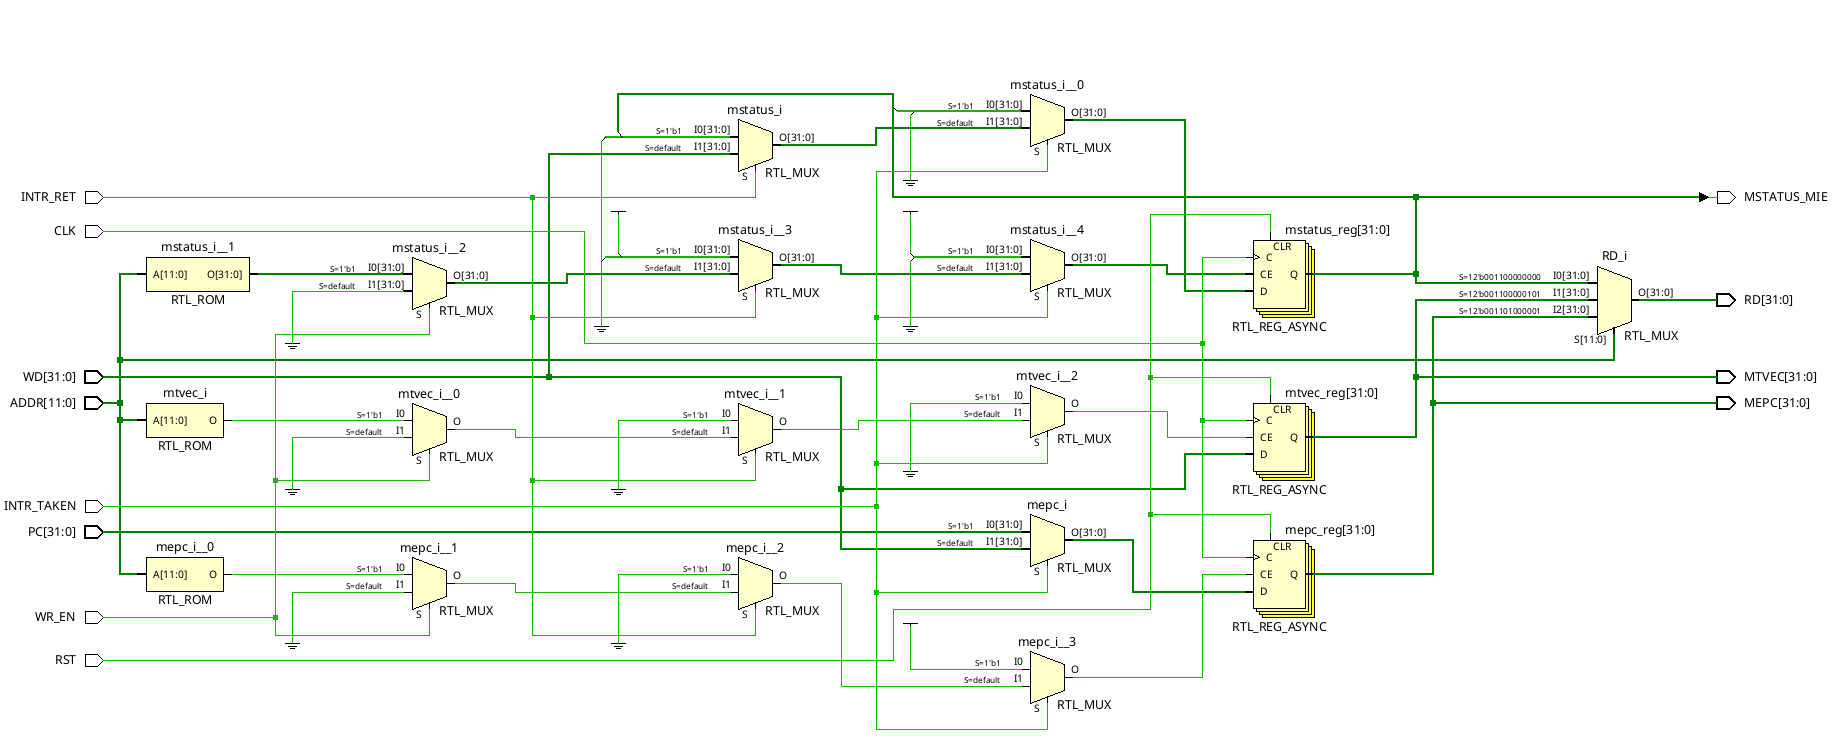
\includegraphics[width=\textwidth]{../03_hardware/hw8/rtl_csr.png}
				\caption{CSR RTL}
			\end{figure}

			\begin{figure}[H]
				\centering
				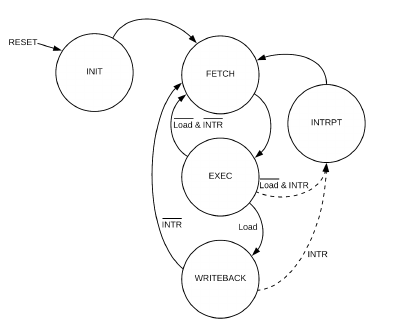
\includegraphics[width=0.7\textwidth]{../03_hardware/hw8/fsm.png}
				\caption{Interrupt-Updated FSM for the Control Unit}
			\end{figure}

			\begin{figure}[H]
				\centering
				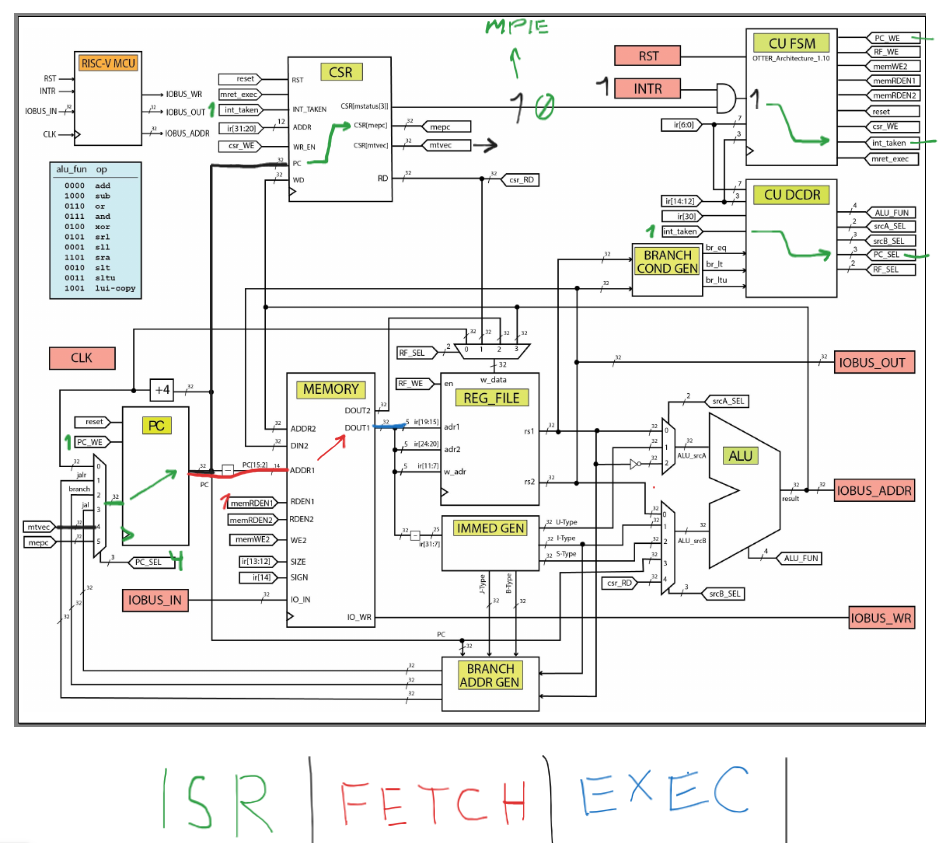
\includegraphics[width=\textwidth]{../03_hardware/hw8/isr_begin.png}
				\caption{Dataflow entering the ISR}
			\end{figure}

			\begin{figure}[H]
				\centering
				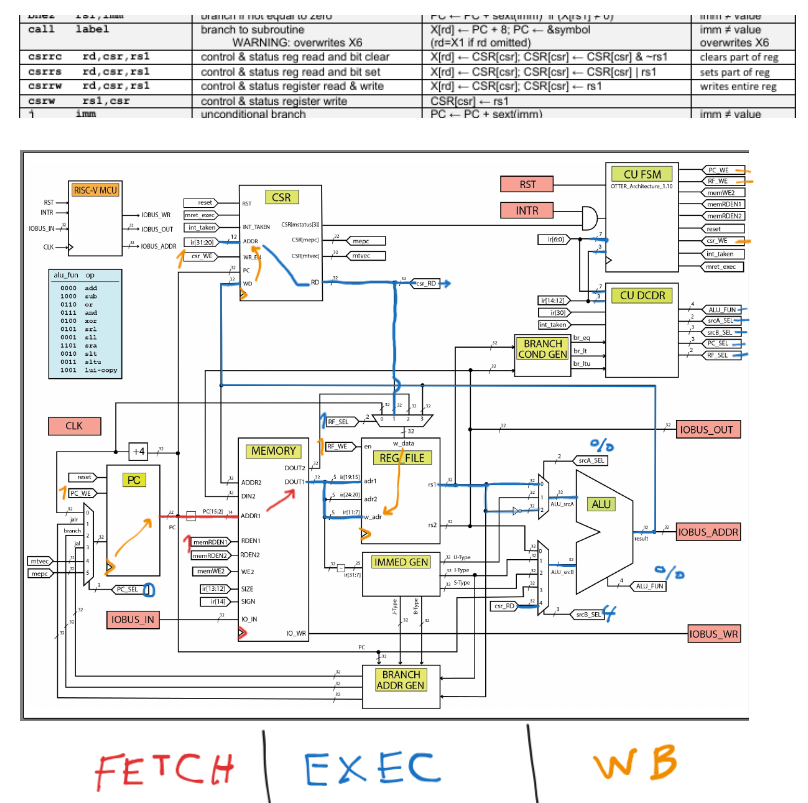
\includegraphics[width=\textwidth]{../03_hardware/hw8/isr_cssrx.png}
				\caption{Dataflow reading/writing the ISR registers}
			\end{figure}

			\begin{figure}[H]
				\centering
				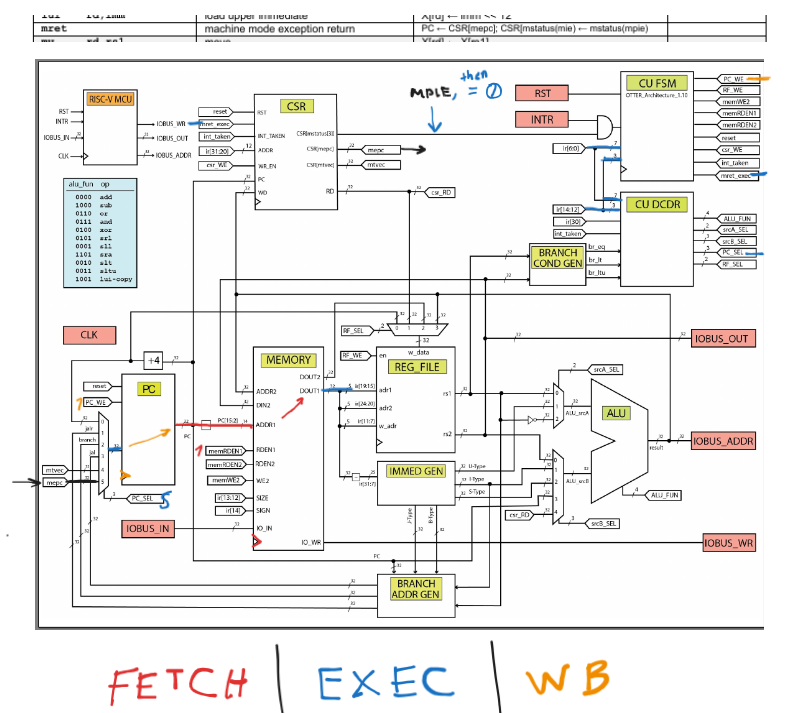
\includegraphics[width=\textwidth]{../03_hardware/hw8/isr_ret.png}
				\caption{Dataflow exiting the ISR}
			\end{figure}

			\begin{figure}[H]
				\centering
				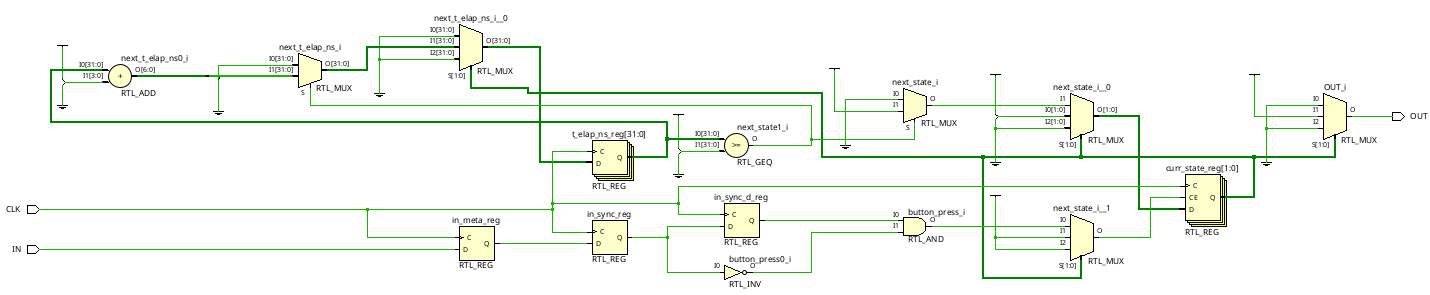
\includegraphics[width=\textwidth]{../03_hardware/hw8/rtl_debounce.png}
				\caption{Debounce OneShot RTL}
			\end{figure}

			\begin{figure}[H]
				\centering
				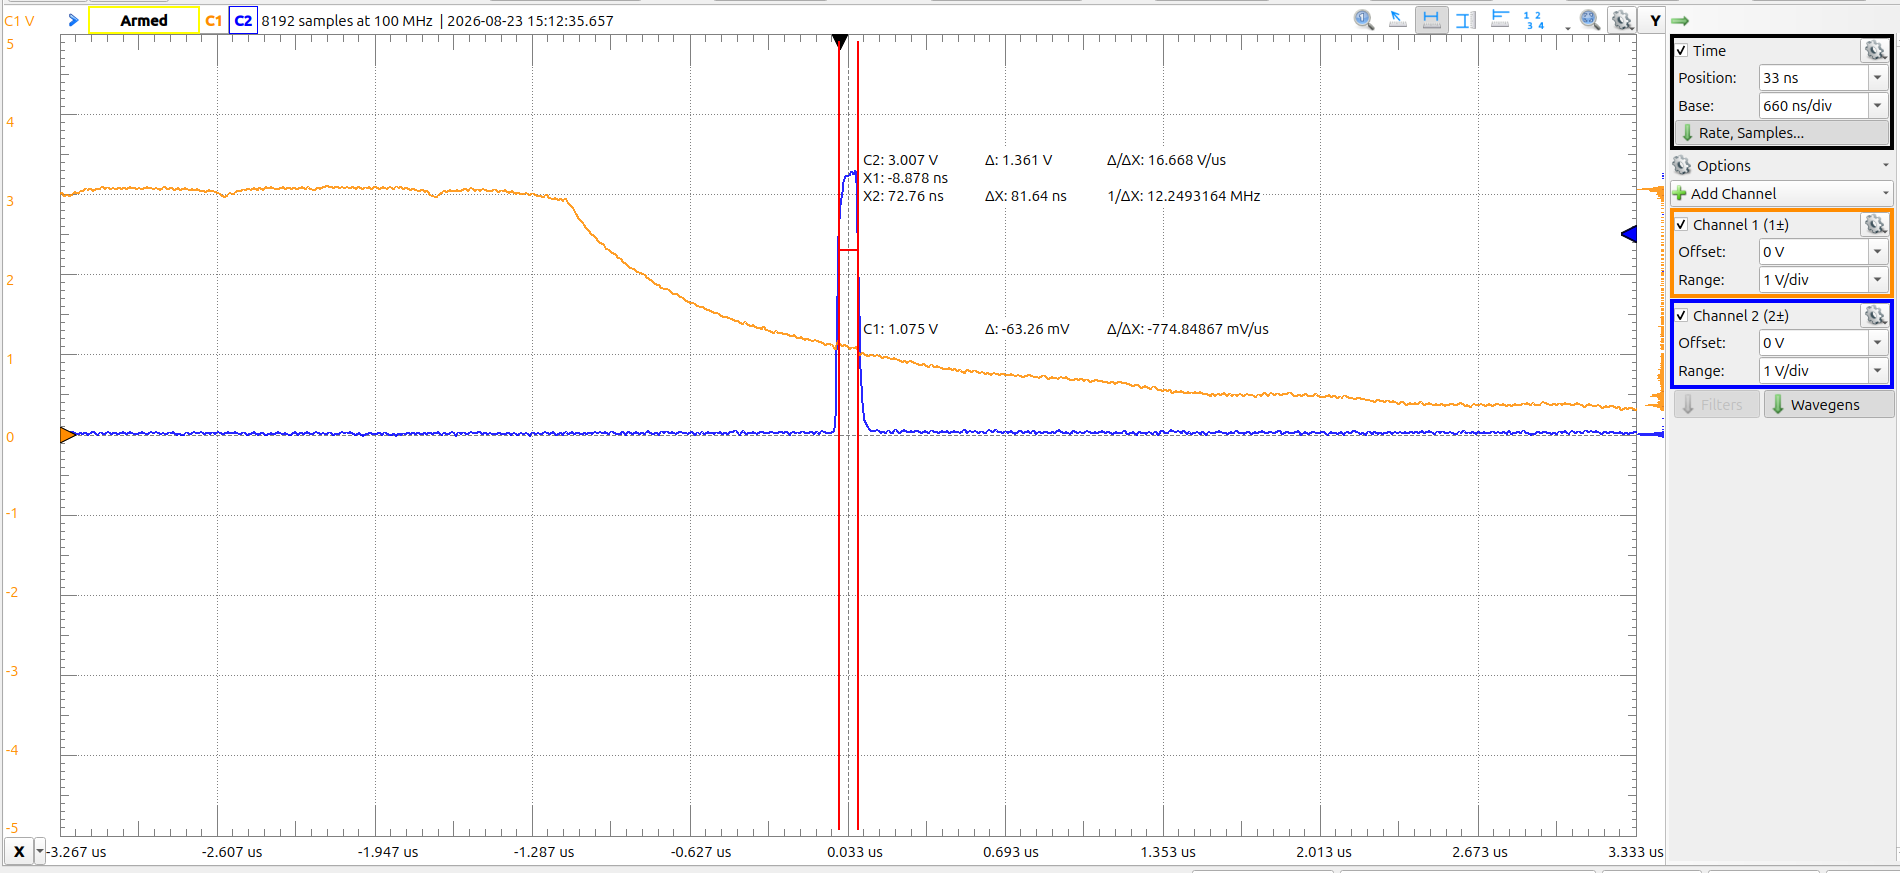
\includegraphics[width=\textwidth]{../03_hardware/hw8/debounce_meas_80ns.png}
				\caption{80ns debounce measurement on hardware}
			\end{figure}

			\begin{itemize}
				\item OTTER WRAPPER rtl \ref{otter:wrap} and test \ref{ottertest:wrap}  
				\item OTTER MCU rtl \ref{otter:mcu} and test \ref{ottertest:mcu}  
				\item OTTER CSR rtl \ref{otter:csr} and test \ref{ottertest:csr}  
				\item OTTER OneShot debounce rtl \ref{otter:debounce} and test \ref{ottertest:debounce}  
				\item Asm hardware test file for Interrupt OTTER WRAPPER \ref{ottertest:interrupt}.
			\end{itemize}

			
			

	\newpage
	\section{Software}

		\subsection{SW1 - Intro to Assembly Lang}

			Note : Assume caller/callee does not need to preserve 
				their respective registers in order to use them. KISS
				method applied for assignment 1. 


			\subsubsection{Part 1}

				"Read three 16-bit unsigned values consecutively from 
					SWITCHES (address 0x11000000), add them together, 
					and output the result to LEDS (address 0x11000020). 
					Assume the input values are 16-bit unsigned values.
					(Assume it is possible for the switches to change 
					between each time they are read)"\\

					Assuming the LEDS input value is limited to 16-bit
					unsigned as well.\\

				\textbf{Flowchart}\\

					\begin{figure}[H]
						\centering
						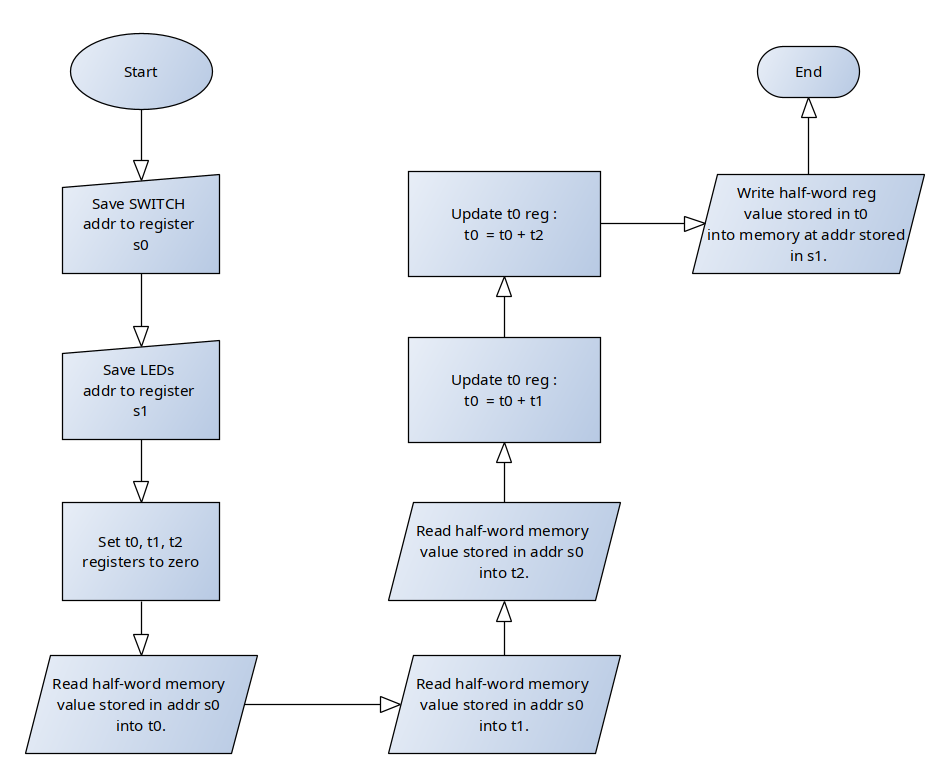
\includegraphics[width=0.8\textwidth]{../02_software/sw1/photos/p1/p1_flow.png}
						\caption{Flow Chart for Part 1}
						\label{fig:p1_flow}
					\end{figure}

				\textbf{Verification Simulations}\\

					\begin{figure}[H]
						\centering
						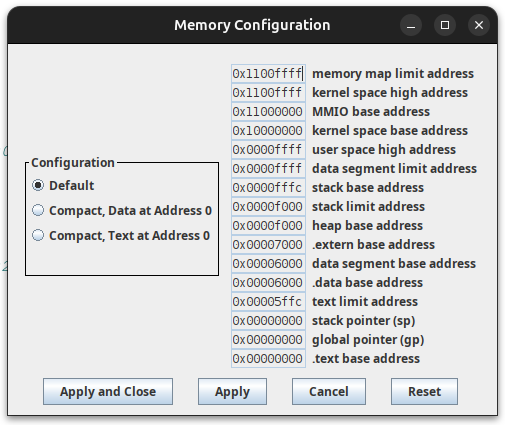
\includegraphics[width=0.6\textwidth]{../02_software/sw1/photos/p1/a1_memconfig.png}
						\caption{RARS Memory Configuration}
						\label{fig:a1_memconfig}
					\end{figure}

					\begin{figure}[H]
						\centering
						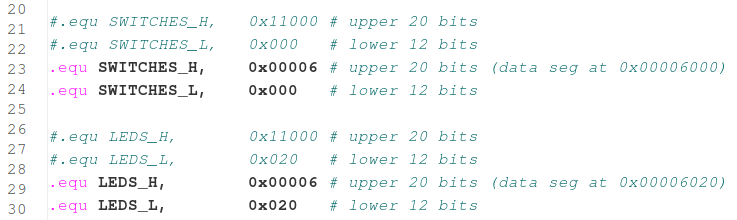
\includegraphics[width=0.8\textwidth]{../02_software/sw1/photos/p1/a1_addr_a.png}
						\caption{Address Correction to work with RARS}
						\label{fig:}
					\end{figure}

					\begin{itemize}
						\item \textbf{Test Case 1}
							\begin{figure}[H]
								\centering
								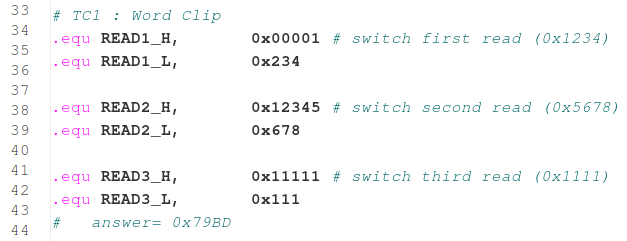
\includegraphics[width=0.8\textwidth]{../02_software/sw1/photos/p1/a1_TC1.png}
								\caption{TC1 given inputs}
								\label{fig:a1_TC1_input}
							\end{figure}

							\begin{figure}[H]
								\centering
								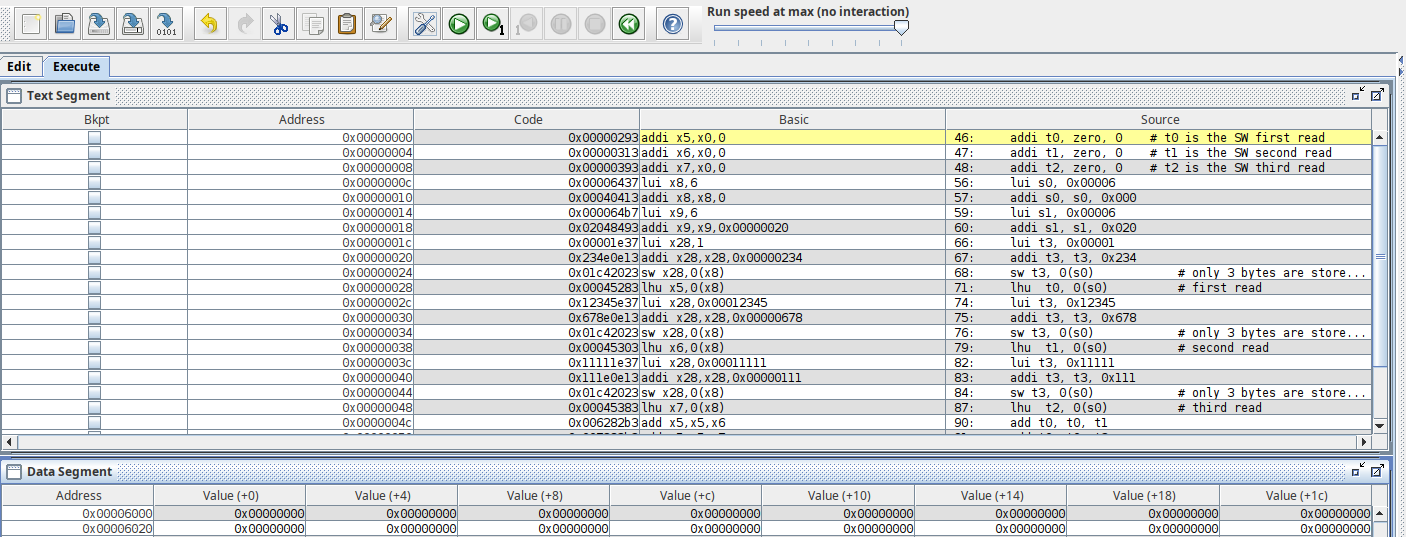
\includegraphics[width=1.0\textwidth]{../02_software/sw1/photos/p1/a1_TC1_before.png}
								\caption{Data segment before executing instructions}
								\label{fig:a1_TC1_before}
							\end{figure}

							\begin{figure}[H]
								\centering
								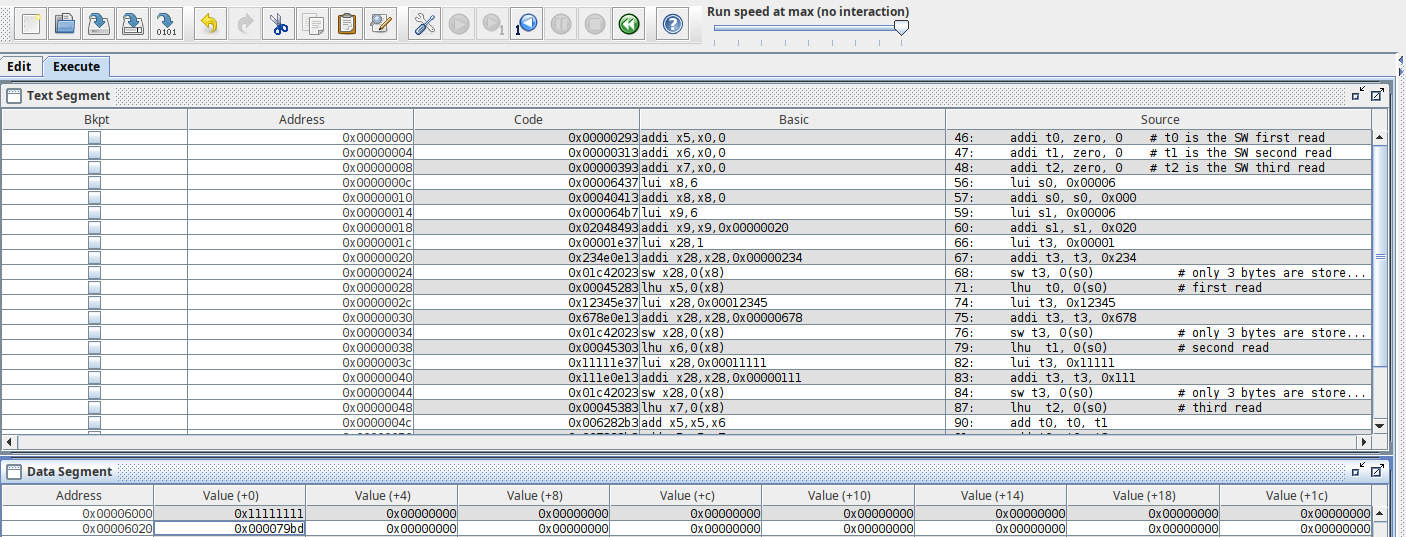
\includegraphics[width=1.0\textwidth]{../02_software/sw1/photos/p1/a1_TC1_after.png}
								\caption{Data segment after executing instructions}
								\label{fig:a1_TC1_after}
							\end{figure}

							Result at LEDS address in \ref{fig:a1_TC1_after} matches the answer in \ref{fig:a1_TC1_input}.


						\item \textbf{Test Case 2}

							\begin{figure}[H]
								\centering
								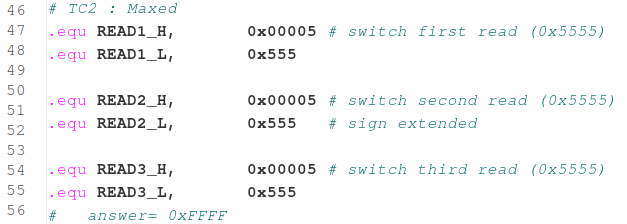
\includegraphics[width=0.8\textwidth]{../02_software/sw1/photos/p1/a1_TC2.png}
								\caption{TC2 given input}
								\label{fig:a1_TC2_input}
							\end{figure}

							\begin{figure}[H]
								\centering
								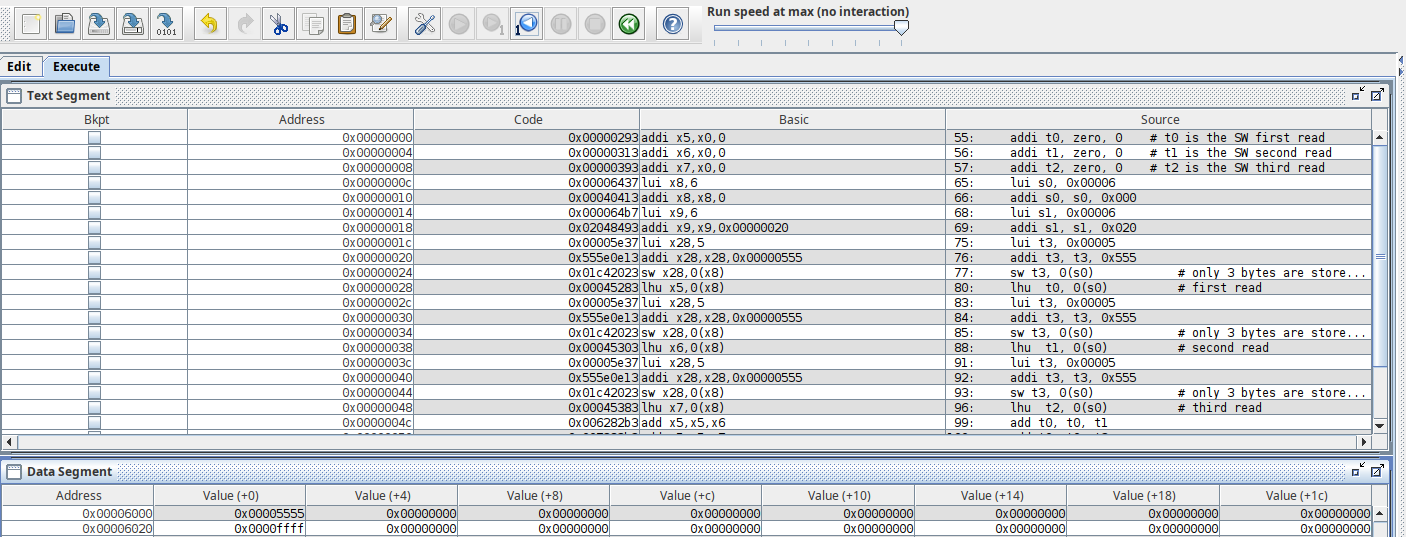
\includegraphics[width=1.0\textwidth]{../02_software/sw1/photos/p1/a1_TC2_after.png}
								\caption{Data segment after executing instructions}
								\label{fig:a1_TC2_after}
							\end{figure}

							Result at LEDS address in \ref{fig:a1_TC2_after} matches the answer in \ref{fig:a1_TC2_input}.

						\item \textbf{Test Case 3}

							\begin{figure}[H]
								\centering
								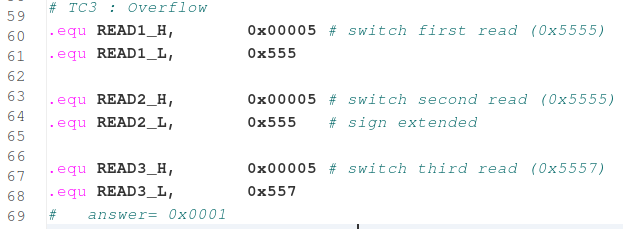
\includegraphics[width=0.8\textwidth]{../02_software/sw1/photos/p1/a1_TC3.png}
								\caption{TC3 given input}
								\label{fig:a1_TC3_input}
							\end{figure}

							\begin{figure}[H]
								\centering
								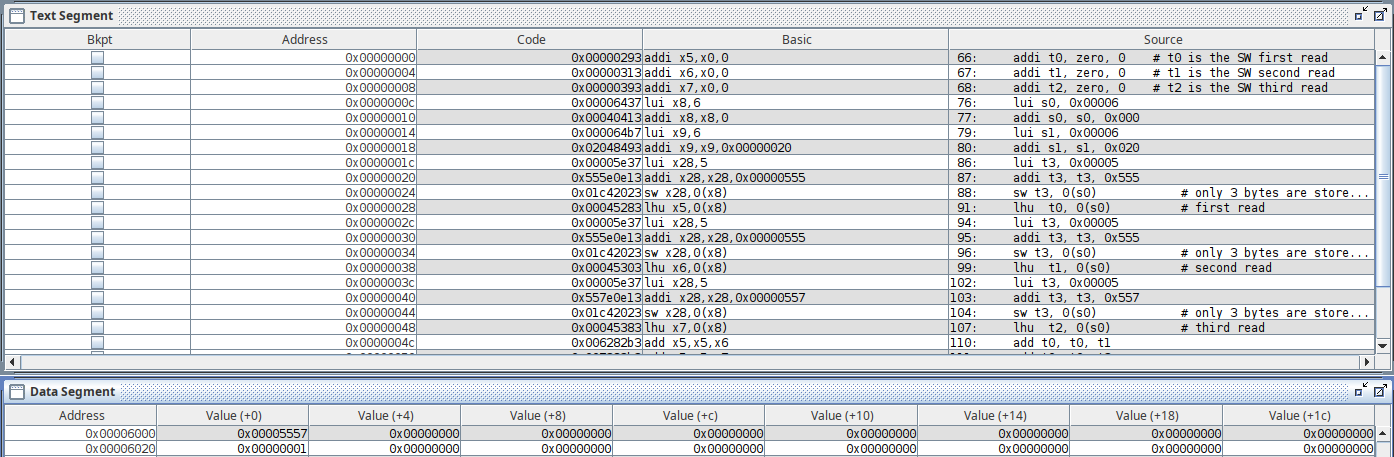
\includegraphics[width=1.0\textwidth]{../02_software/sw1/photos/p1/a1_TC3_after.png}
								\caption{Data segment after executing instructions}
								\label{fig:a1_TC3_after}
							\end{figure}

							Result at LEDS address in \ref{fig:a1_TC3_after} matches the answer in \ref{fig:a1_TC3_input}.

						\item \textbf{Test Case 4}

							\begin{figure}[H]
								\centering
								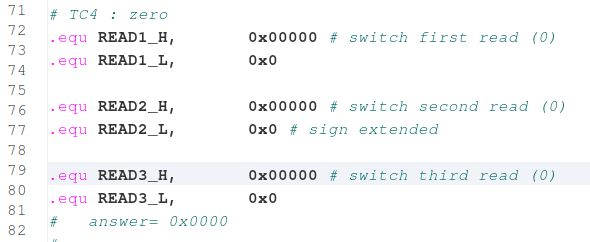
\includegraphics[width=0.8\textwidth]{../02_software/sw1/photos/p1/a1_TC4.png}
								\caption{TC4 given input}
								\label{fig:a1_TC4_input}
							\end{figure}

							\begin{figure}[H]
								\centering
								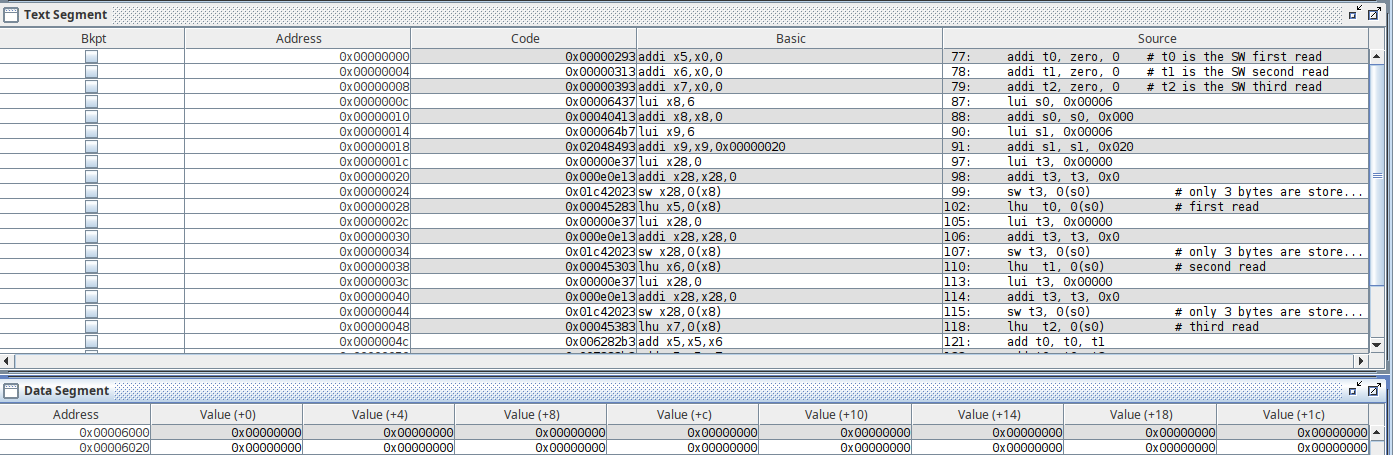
\includegraphics[width=1.0\textwidth]{../02_software/sw1/photos/p1/a1_TC4_after.png}
								\caption{Data segment after executing instructions}
								\label{fig:a1_TC4_after}
							\end{figure}

							Result at LEDS address in \ref{fig:a1_TC4_after} matches the answer in \ref{fig:a1_TC4_input}.

						\item \textbf{Test Case 5}

							\begin{figure}[H]
								\centering
								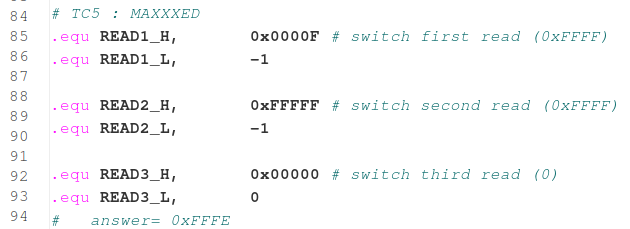
\includegraphics[width=0.8\textwidth]{../02_software/sw1/photos/p1/a1_TC5.png}
								\caption{TC5 given input}
								\label{fig:a1_TC5_input}
							\end{figure}

							\begin{figure}[H]
								\centering
								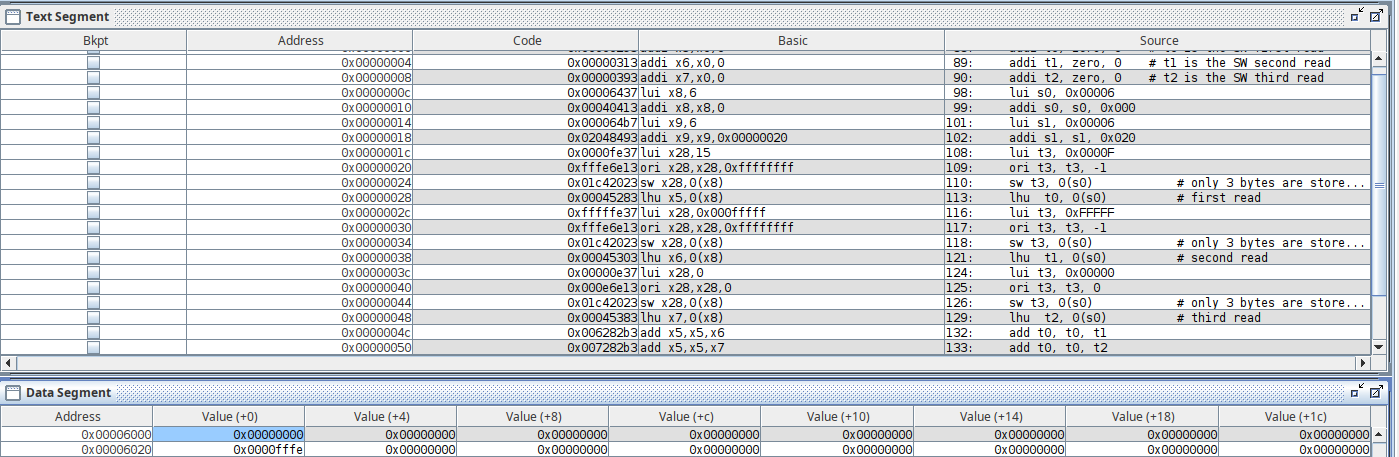
\includegraphics[width=1.0\textwidth]{../02_software/sw1/photos/p1/a1_TC5_after.png}
								\caption{Data segment after executing instructions}
								\label{fig:a1_TC5_after}
							\end{figure}

							Result at LEDS address in \ref{fig:a1_TC5_after} matches the answer in \ref{fig:a1_TC5_input}.

						\item \textbf{Test Case 6}

							\begin{figure}[H]
								\centering
								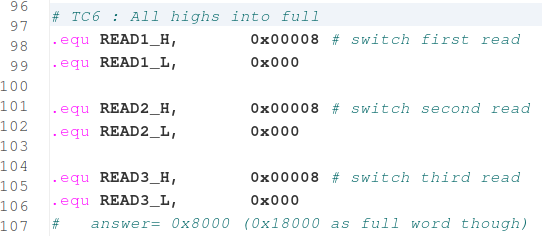
\includegraphics[width=0.8\textwidth]{../02_software/sw1/photos/p1/a1_TC6.png}
								\caption{TC6 given input}
								\label{fig:a1_TC6_input}
							\end{figure}

							\begin{figure}[H]
								\centering
								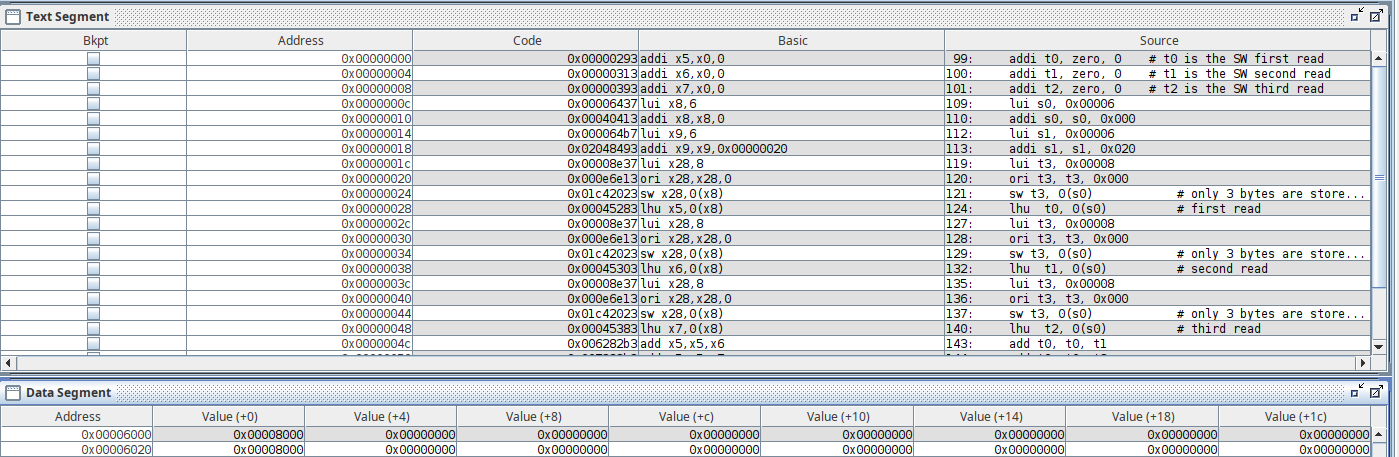
\includegraphics[width=1.0\textwidth]{../02_software/sw1/photos/p1/a1_TC6_after.png}
								\caption{Data segment after executing instructions}
								\label{fig:a1_TC6_after}
							\end{figure}

							Result at LEDS address in \ref{fig:a1_TC6_after} matches the answer in \ref{fig:a1_TC6_input}.

					\end{itemize}

				\textbf{Assembly Source Code}\\
					\lstinputlisting[language={[riscv]Assembler}, captionpos=top,
											caption={Question 1 of SW1},
											breaklines=false]{../02_software/sw1/sw1_1.asm}


			\subsubsection{Part 2}

				"Read an input from SWITCHES (address 0x11000000). 
					Assume the input is a 16-bit signed value in 2’s complement 
					(RC). Change the sign of the input and output the result
					to LEDS (address 0x11000020). The result should also be
					a 16-bit signed value in 2’s complement (RC)."\\

				\textbf{Flowchart}
					\begin{figure}[H]
						\centering
						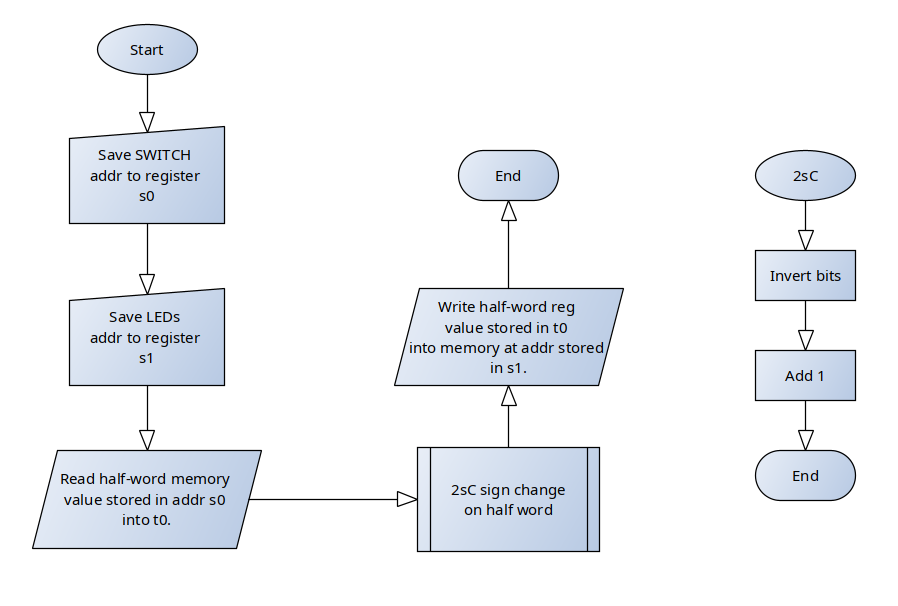
\includegraphics[width=0.8\textwidth]{../02_software/sw1/photos/p2/p2_flow.png}
						\caption{Flow Chart for Part 2}
						\label{fig:p2_flow}
					\end{figure}


				\textbf{Verification Simulations}\\
					Test cases passed with definitions defined in code below.

					\begin{figure}[H]
						\centering
						\begin{subfigure}{0.4\textwidth}
							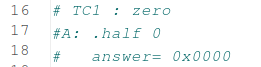
\includegraphics[width=\textwidth]{../02_software/sw1/photos/p2/a1p2_TC1.png}
						\end{subfigure}
						\begin{subfigure}{0.4\textwidth}
							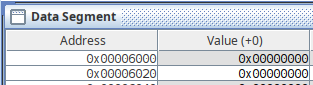
\includegraphics[width=\textwidth]{../02_software/sw1/photos/p2/a1p2_TC1_after.png}
						\end{subfigure}
						\caption{IO and Data Segment of TC1}
						\label{fig:a1p2_TC1}
					\end{figure}

					\begin{figure}[H]
						\centering
						\begin{subfigure}{0.4\textwidth}
							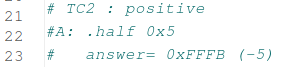
\includegraphics[width=\textwidth]{../02_software/sw1/photos/p2/a1p2_TC2.png}
						\end{subfigure}
						\begin{subfigure}{0.4\textwidth}
							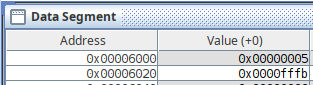
\includegraphics[width=\textwidth]{../02_software/sw1/photos/p2/a1p2_TC2_after.png}
						\end{subfigure}
						\caption{IO and Data Segment of TC2}
						\label{fig:a1p2_TC2}
					\end{figure}

					\begin{figure}[H]
						\centering
						\begin{subfigure}{0.4\textwidth}
							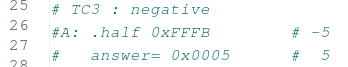
\includegraphics[width=\textwidth]{../02_software/sw1/photos/p2/a1p2_TC3.png}
						\end{subfigure}
						\begin{subfigure}{0.4\textwidth}
							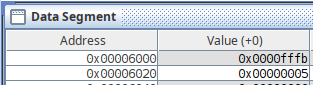
\includegraphics[width=\textwidth]{../02_software/sw1/photos/p2/a1p2_TC3_after.png}
						\end{subfigure}
						\caption{IO and Data Segment of TC3}
						\label{fig:a1p2_TC3}
					\end{figure}

					\begin{figure}[H]
						\centering
						\begin{subfigure}{0.4\textwidth}
							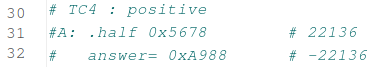
\includegraphics[width=\textwidth]{../02_software/sw1/photos/p2/a1p2_TC4.png}
						\end{subfigure}
						\begin{subfigure}{0.4\textwidth}
							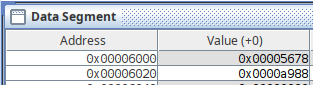
\includegraphics[width=\textwidth]{../02_software/sw1/photos/p2/a1p2_TC4_after.png}
						\end{subfigure}
						\caption{IO and Data Segment of TC4}
						\label{fig:a1p2_TC4}
					\end{figure}

					\begin{figure}[H]
						\centering
						\begin{subfigure}{0.4\textwidth}
							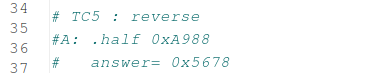
\includegraphics[width=\textwidth]{../02_software/sw1/photos/p2/a1p2_TC5.png}
						\end{subfigure}
						\begin{subfigure}{0.4\textwidth}
							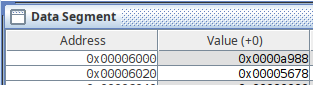
\includegraphics[width=\textwidth]{../02_software/sw1/photos/p2/a1p2_TC5_after.png}
						\end{subfigure}
						\caption{IO and Data Segment of TC5}
						\label{fig:a1p2_TC5}
					\end{figure}

					\begin{figure}[H]
						\centering
						\begin{subfigure}{0.4\textwidth}
							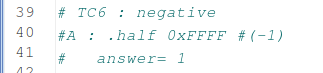
\includegraphics[width=\textwidth]{../02_software/sw1/photos/p2/a1p2_TC6.png}
						\end{subfigure}
						\begin{subfigure}{0.4\textwidth}
							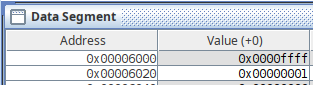
\includegraphics[width=\textwidth]{../02_software/sw1/photos/p2/a1p2_TC6_after.png}
						\end{subfigure}
						\caption{IO and Data Segment of TC6}
						\label{fig:a1p2_TC6}
					\end{figure}

					\begin{figure}[H]
						\centering
						\begin{subfigure}{0.4\textwidth}
							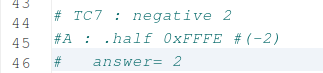
\includegraphics[width=\textwidth]{../02_software/sw1/photos/p2/a1p2_TC7.png}
						\end{subfigure}
						\begin{subfigure}{0.4\textwidth}
							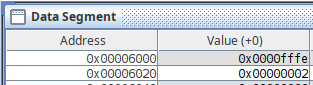
\includegraphics[width=\textwidth]{../02_software/sw1/photos/p2/a1p2_TC7_after.png}
						\end{subfigure}
						\caption{IO and Data Segment of TC7}
						\label{fig:a1p2_TC7}
					\end{figure}

					\begin{figure}[H]
						\centering
						\begin{subfigure}{0.4\textwidth}
							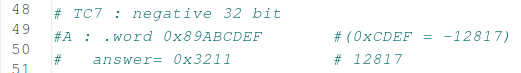
\includegraphics[width=\textwidth]{../02_software/sw1/photos/p2/a1p2_TC8.png}
						\end{subfigure}
						\begin{subfigure}{0.4\textwidth}
							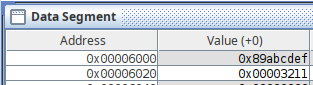
\includegraphics[width=\textwidth]{../02_software/sw1/photos/p2/a1p2_TC8_after.png}
						\end{subfigure}
						\caption{IO and Data Segment of TC8}
						\label{fig:a1p2_TC8}
					\end{figure}

				\textbf{Assembly Code}
					\lstinputlisting[language={[riscv]Assembler}, captionpos=top,
									caption={Question 2 of SW1},
									breaklines=false]{../02_software/sw1/sw1_2.asm}

		\newpage
		\subsection{SW2 - Conditional Statements}
			\begin{figure}[H]
				\centering
				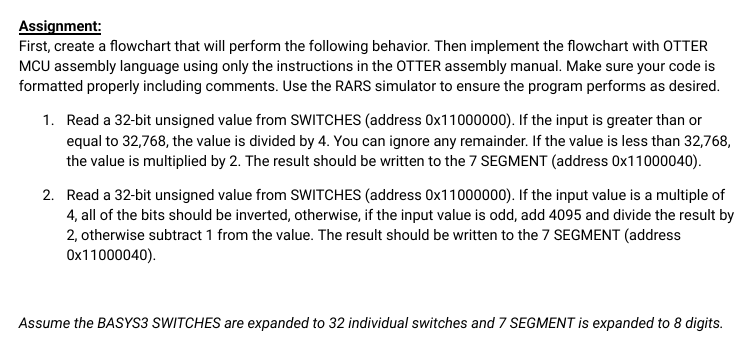
\includegraphics[width=0.8\textwidth]{../02_software/sw2/assignment.png}
				\caption{Questions to address}
				\label{fig:-02_software-sw2-assignment-png}
			\end{figure}

			\subsubsection{Part 1}

				\begin{figure}[H]
					\centering
					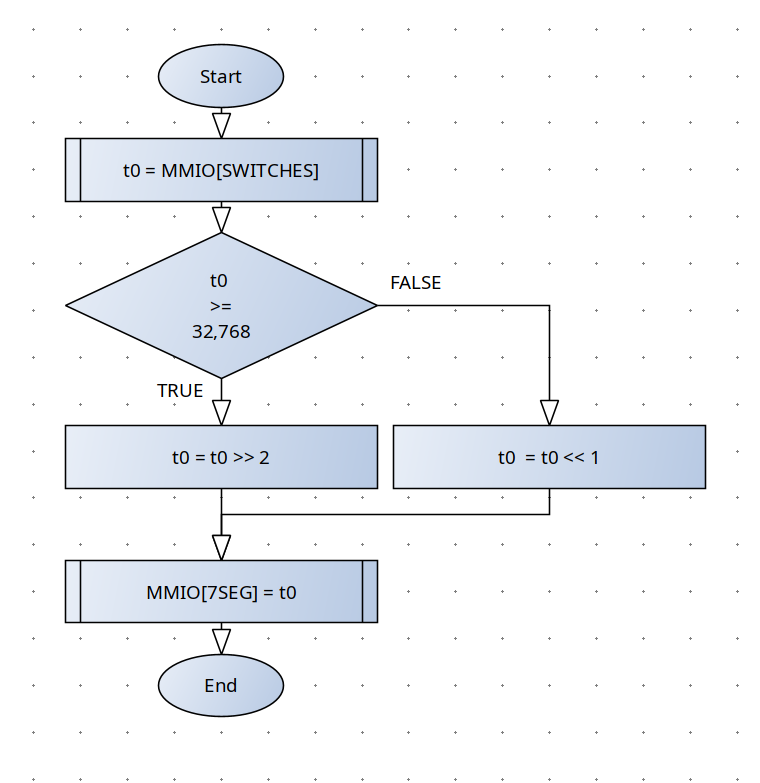
\includegraphics[width=0.6\textwidth]{../02_software/sw2/p1_photos/flow.png}
					\caption{Flow chart for part 1}
					\label{fig:-02_software-sw2-p1_photos-flow-png}
				\end{figure}	

				\begin{table}[h]
					\centering
					\label{tab:label}
					\begin{tabular}{||c|c|c|c|c||}
						\hline
					\textbf{TC\#} & \textbf{Desc} & \textbf{Given MMIO[SWITCHES]} & \textbf{Correct MMIO[7SEG]} & \textbf{Result}\\ \hline
						1 & Lowest unsigned val & $0$ & $0$ & Passed \\ \hline
						2 & Below boundary & $0xFFF$ & $0x1FFE$ & Passed \\ \hline
						3 & 1 before boundary & $0x7FFF$ & $0xFFFE$ & Passed \\ \hline
						4 & On boundary & $0x8000$ & $0x2000$ & Passed \\ \hline
						5 & 1 above boundary & $0x8001$ & $0x2000$ & Passed \\ \hline
						6 & Above boundary & $0x12345678$ & $0x048D159E$ & Passed \\ \hline
						7 & 32-bit unsigned ceiling & $0xFFFFFFFF$ & $0x3FFFFFFF$ & Passed \\ \hline
						\hline
					\end{tabular}
					\caption{Test cases for part 1}
				\end{table}

				\begin{figure}[H]
					\centering
					\lstinputlisting[language={[riscv]Assembler}, captionpos=top,
									caption={sw2\_p1.asm},
									breaklines=false]{../02_software/sw2/sw2_p1.asm}
					\caption{Assembly code for SW2 part 1}
					\label{fig:}
				\end{figure}

			\subsubsection{Part 2}

				\begin{figure}[H]
					\centering
					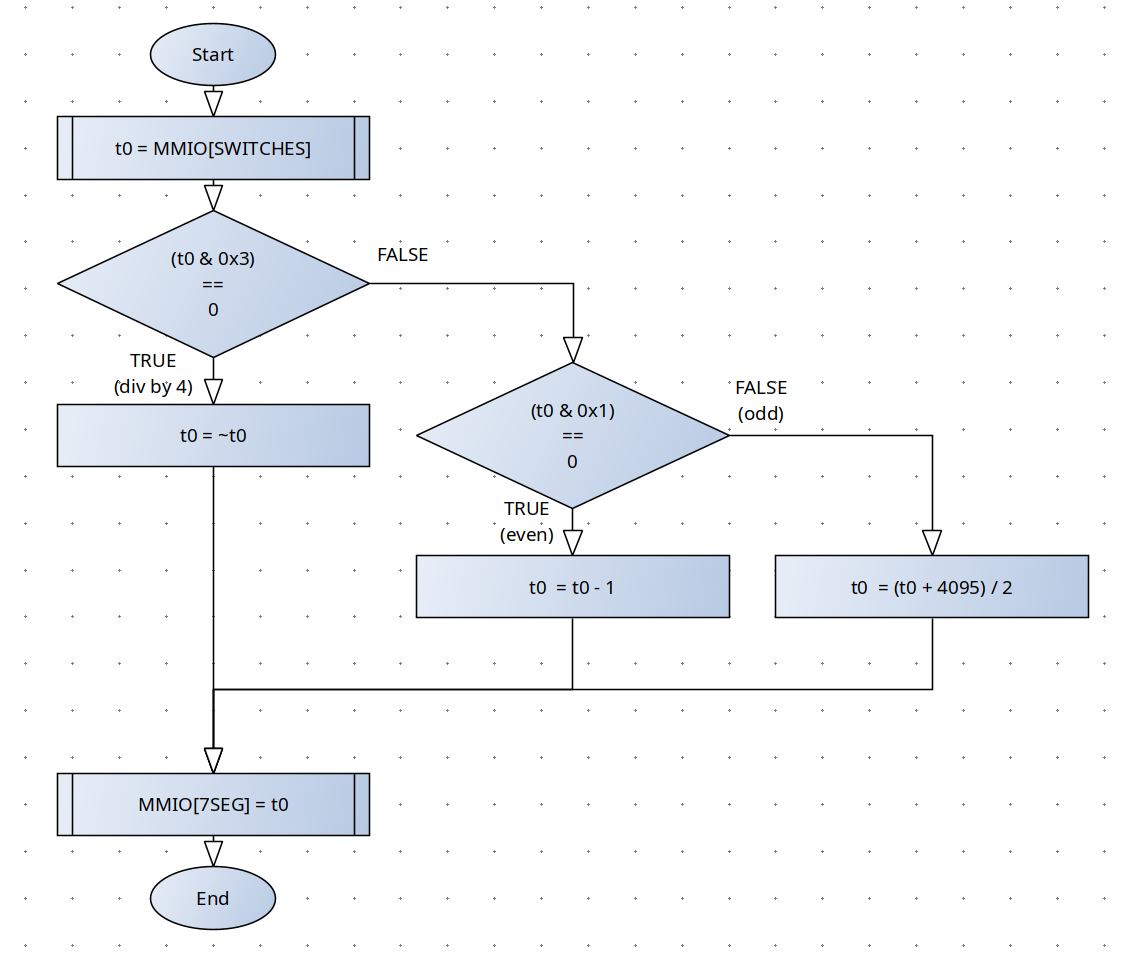
\includegraphics[width=0.6\textwidth]{../02_software/sw2/p2_photos/flow.png}
					\caption{Flow chart for part 2}
					\label{fig:-02_software-sw2-p2_photos-flow-png}
				\end{figure}	

				\begin{table}[h]
					\centering
					\label{tab:label}
					\begin{tabular}{||c|c|c|c|c||}
						\hline
					\textbf{TC\#} & \textbf{Desc} & \textbf{Given MMIO[SWITCHES]} & \textbf{Correct MMIO[7SEG]} & \textbf{Result}\\ \hline
						1 & Zero is div by 4 & $0$ & $0xFFFF FFFF$ & Passed \\ \hline
						2 & Two is even & $0x2$ & $0x1$ & Passed \\ \hline
						3 & One is odd & $0x1$ & $0x0800$ & Passed \\ \hline
						4 & 32-bit unsinged ceiling & $0xFFFFFFFF$ & $0x07FF$ & Passed \\ \hline
						5 & Div by 4 near ceiling & $0xFFFFFFFC$ & $0x3$ & Passed \\ \hline
						6 & Odd near ceiling & $0xFFFFFFFD$ & $0x07FE$ & Passed \\ \hline
						7 & Even near ceiling & $0xFFFFFFFE$ & $0xFFFFFFFD$ & Passed \\ \hline
						\hline
					\end{tabular}
					\caption{Test cases for part 1}
				\end{table}

				\begin{figure}[H]
					\centering
					\lstinputlisting[language={[riscv]Assembler}, captionpos=top,
									caption={sw2\_p2.asm},
									breaklines=false]{../02_software/sw2/sw2_p2.asm}
					\caption{Assembly code for SW2 part 2}
					\label{fig:}
				\end{figure}

		\newpage
		\subsection{SW3 - Loops}
			\begin{figure}[H]
				\centering
				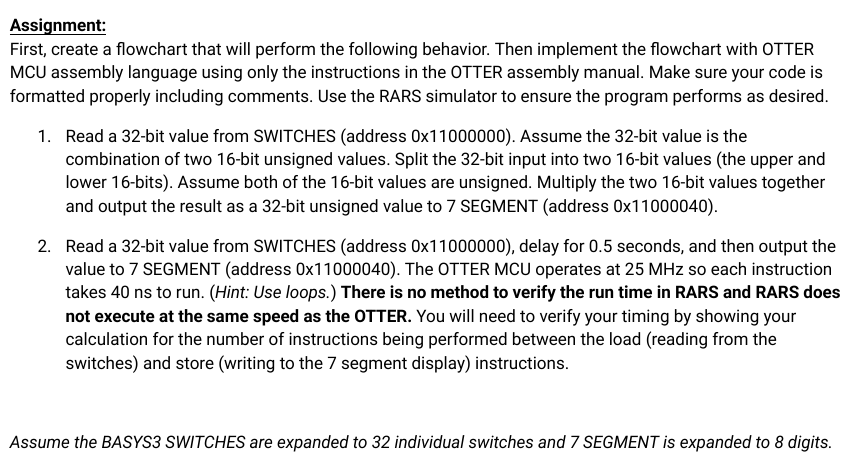
\includegraphics[width=0.8\textwidth]{../02_software/sw3/assignment.png}
				\caption{Questions to address}
				\label{fig:-02_software-sw3-assignment-png}
			\end{figure}

			\subsubsection{Part 1}

				\begin{figure}[H]
					\centering
					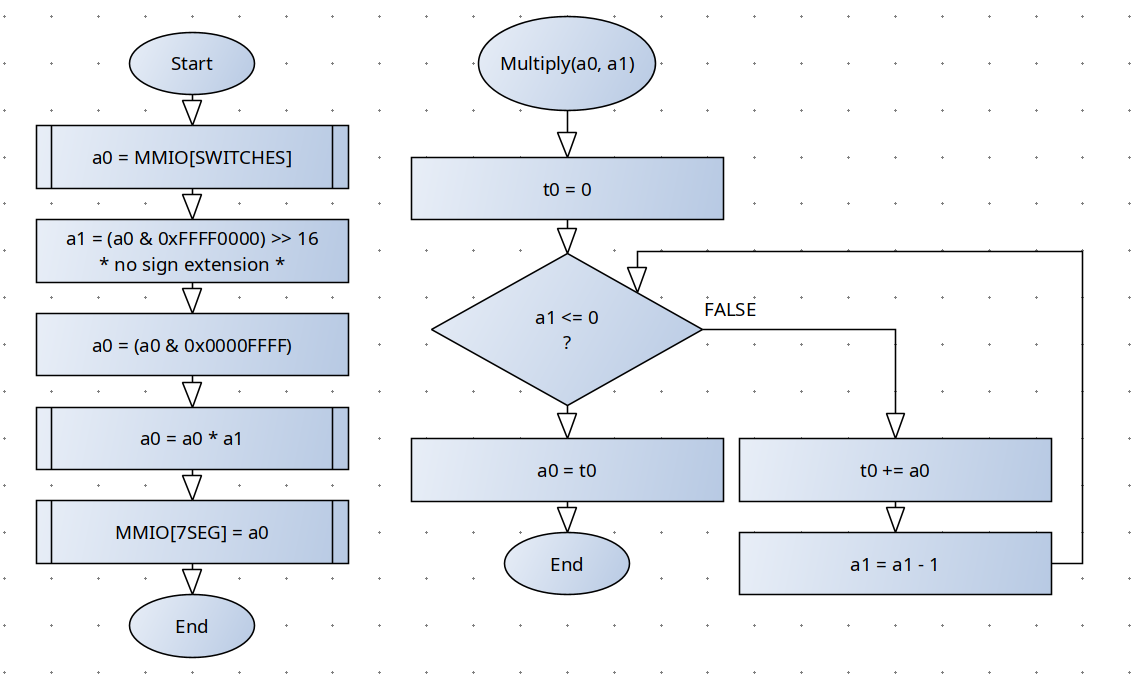
\includegraphics[width=0.6\textwidth]{../02_software/sw3/p1_photos/flow.png}
					\caption{Flow chart for part 1}
					\label{fig:-02_software-sw3-p1_photos-flow-png}
				\end{figure}	

				\begin{table}[h]
					\centering
					\label{tab:label}
					\begin{tabular}{||c|c|c|c|c||}
						\hline
					\textbf{TC\#} & \textbf{Desc} & \textbf{Given MMIO[SWITCHES]} & \textbf{Correct MMIO[7SEG]} & \textbf{Result}\\ \hline
						1 & Zero & $0x0000\_0000$ & $0x0000\_0000$ & Passed \\ \hline
						2 & Zero + One & $0x0000\_0001$ & $0x0000\_0000$ & Passed \\ \hline
						3 & One + Zero & $0x0001\_0000$ & $0x0000\_0000$ & Passed \\ \hline
						4 & One + One & $0x0001\_0001$ & $0x0000\_0001$ & Passed \\ \hline
						5 & num1 & $0x0013\_0004$ & $0x0000\_004C$ & Passed \\ \hline
						6 & num1 reverse & $0x0004\_0013$ & $0x0000\_004C$ & Passed \\ \hline
						7 & shift 1 & $0xFFFF\_FFFF$ & $0xFFFE\_0001$ & Passed \\ \hline
						8 & shift 2& $0x0010\_FFFF$ & $0x000F\_FFF0$ & Passed \\ \hline
						9 & shift 3 & $0x0100\_FFFF$ & $0x00FF\_FF00$ & Passed \\ \hline
						\hline
					\end{tabular}
					\caption{Test cases for part 1}
				\end{table}

				\lstinputlisting[
					language={[riscv]Assembler},
					captionpos=top,
					caption={sw3\_p1.asm},
					breaklines=false]
					{../02_software/sw3/sw3_p1.asm}

			\subsubsection{Part 2}

				\begin{figure}[H]
					\centering
					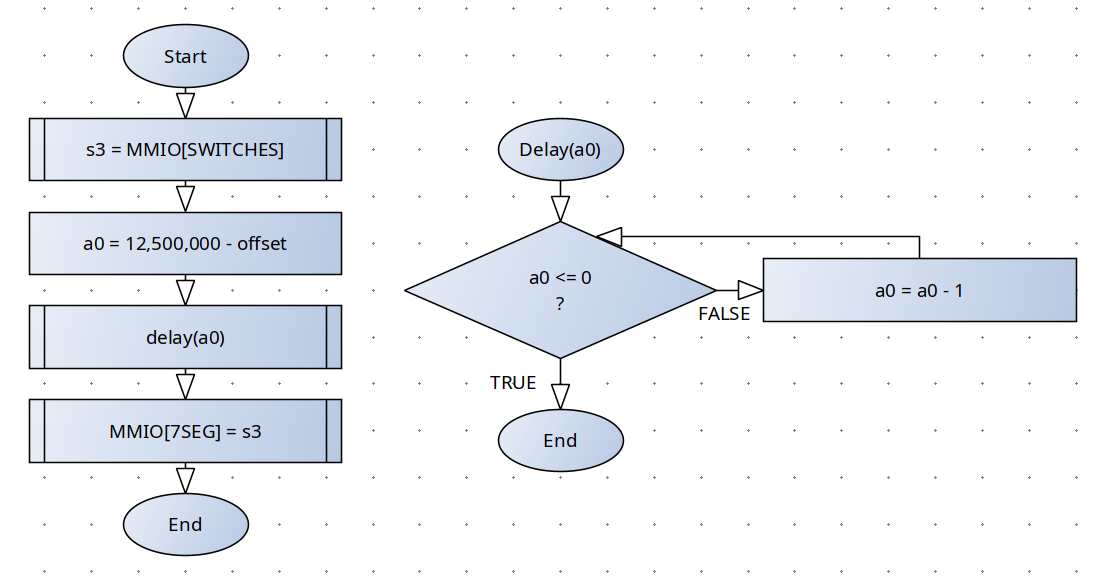
\includegraphics[width=0.6\textwidth]{../02_software/sw3/p2_photos/flow.png}
					\caption{Flow chart for part 2}
					\label{fig:-02_software-sw3-p2_photos-flow-png}
				\end{figure}	

				Consider the following calculations
				\begin{align*}
					12.5 \cdot 10^6 \text{ instr} &= 0.5s \cdot \frac{\text{instr}}{40ns} \cdot \frac{10^9 ns}{1 s}\\
					&= \text{0x00BE\_BC20} \\
				\end{align*}

				\begin{itemize}
					\item There are 13 instructions, after reading
							from SWTICHES, that are only executed once.
							Lets refer to these instructions as bias s.t.
							$b = 13$.
					\item There are 3 instruction in our delay loop s.t.
							$m = 3$.
				\end{itemize}

				Now lets relate our instructions to the instruction layout
				s.t. we identify how many times we actually need to loop.

				\begin{align*}
					3m + b &= 12.5 \cdot 10^9 \\
					m &= \frac{12,500,000 - 13}{3} \\
					&= 4,166,663 \\
				\end{align*}

				Rather than use this number in directly, I opted to write
				the constant in terms of total instructions needed against
				how many loops we need. 

				\begin{align*}
					\text{offset} &= 12.5 \cdot 10^9 - m \\
					&= 8,333,337\\
					&= \text{0x007F\_2819} \\
				\end{align*}
								
				
				\lstinputlisting[
					language={[riscv]Assembler},
					captionpos=top,
					caption={Assembly code for sw3\_p2.asm},
					label={code:sw3p2},
					breaklines=false]
					{../02_software/sw3/sw3_p2.asm}


		\newpage
		\subsection{SW4 - Arrays}
			\begin{figure}[H]
				\centering
				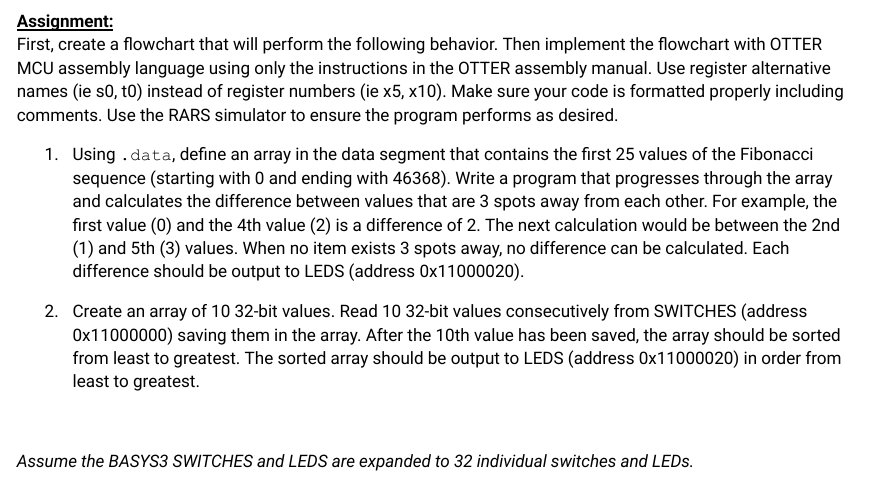
\includegraphics[width=0.8\textwidth]{../02_software/sw4/assignment.png}
				\caption{Questions to address}
				\label{fig:-02_software-sw4-assignment-png}
			\end{figure}

			\begin{figure}[H]
				\centering
				\includegraphics[width=0.6\textwidth]{../02_software/sw4/memconfig.png}
				\caption{Memory Map for this Assignment}
				\label{fig:-02_software-sw4-memconfig-png}
			\end{figure}


			\subsubsection{Part 1}

				\begin{figure}[H]
					\centering
					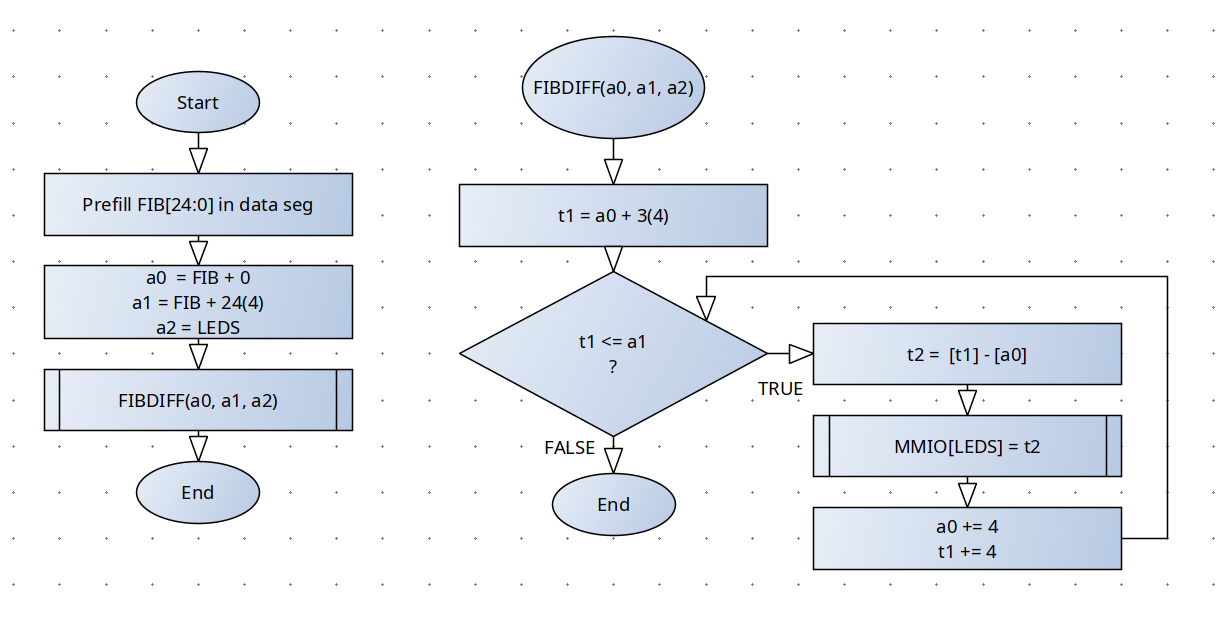
\includegraphics[width=0.6\textwidth]{../02_software/sw4/p1_flow.png}
					\caption{Flow chart for part 1}
					\label{fig:-02_software-sw4-p1_photos-flow-png}
				\end{figure}	

				\lstinputlisting[
					language={[riscv]Assembler},
					captionpos=top,
					caption={sw4\_p1.asm},
					breaklines=false]
					{../02_software/sw4/sw4_p1.asm}

			\subsubsection{Part 2}

				\begin{figure}[H]
					\centering
					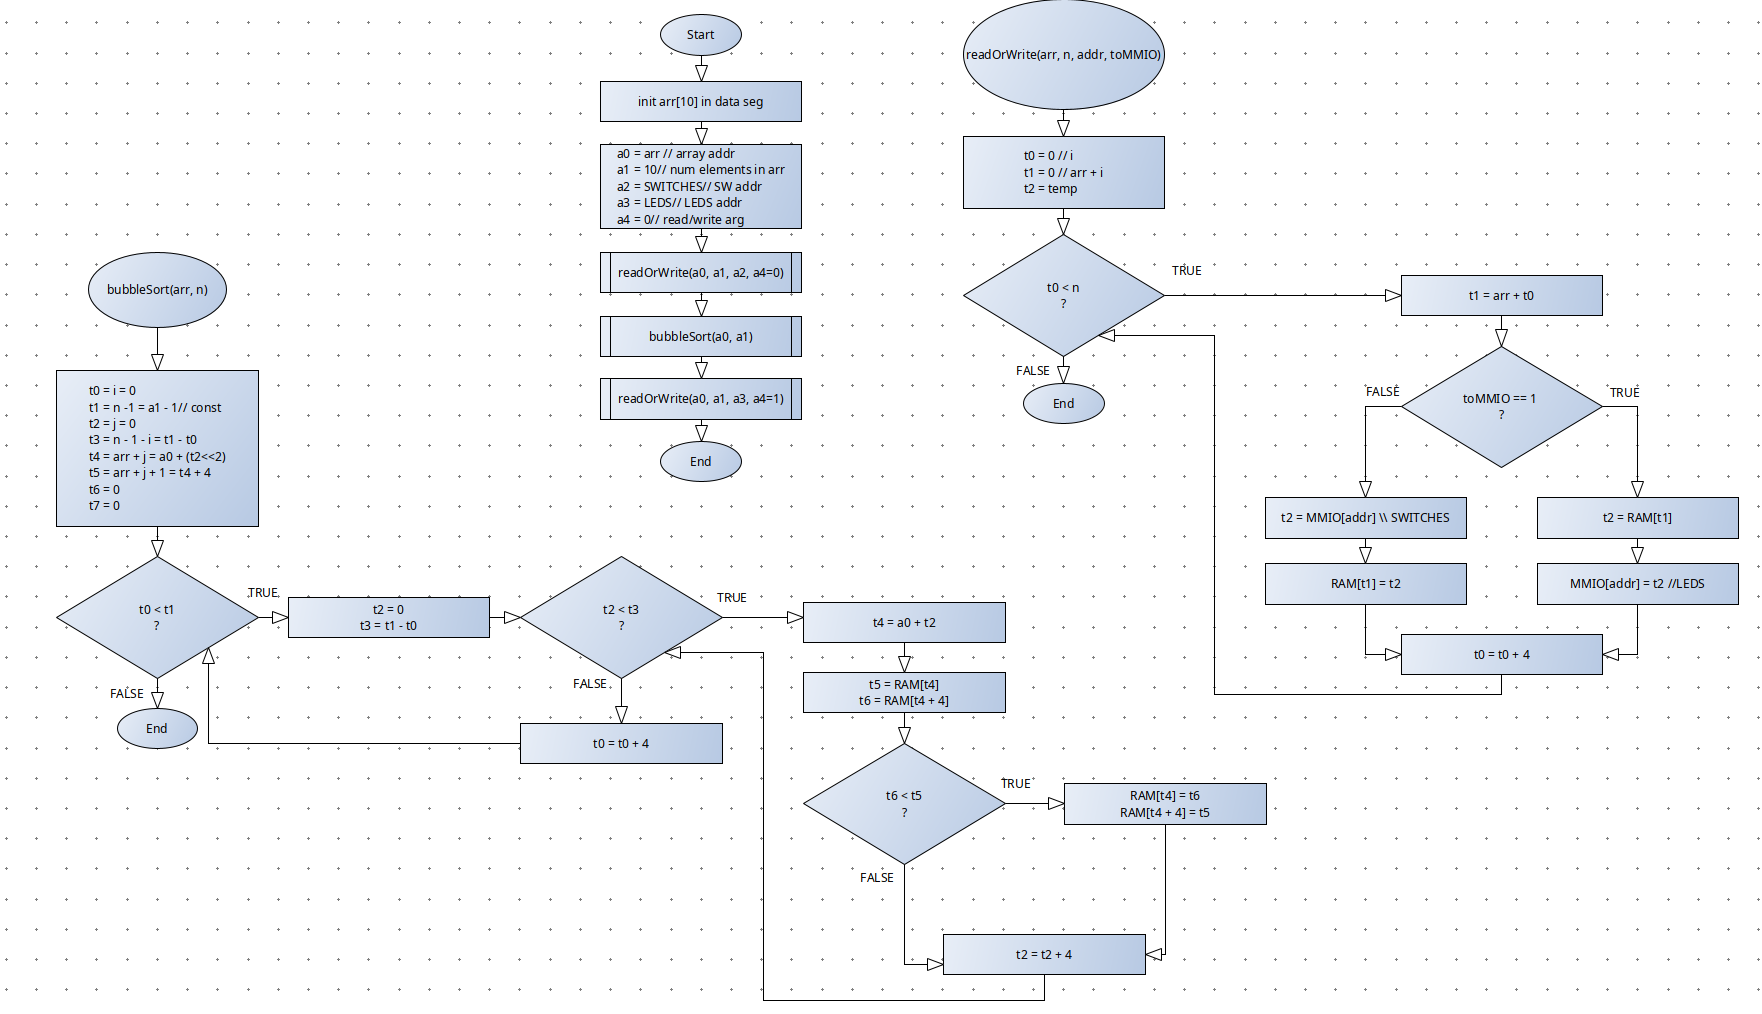
\includegraphics[width=\textwidth]{../02_software/sw4/p2_flow.png}
					\caption{Flow chart for part 2}
					\label{fig:-02_software-sw4-p2_photos-flow-png}
				\end{figure}	
				
				\lstinputlisting[
					language={[riscv]Assembler},
					captionpos=top,
					caption={Assembly code for sw4\_p2.asm},
					label={code:sw4p2},
					breaklines=false]
					{../02_software/sw4/sw4_p2.asm}


		\newpage
		\subsection{SW5 - Division and Stacks}
			\begin{figure}[H]
				\centering
				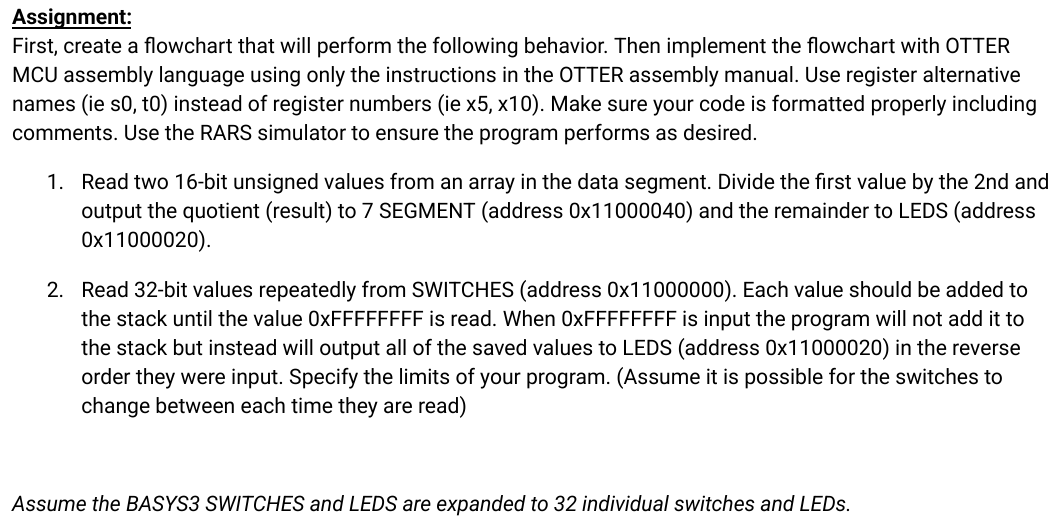
\includegraphics[width=0.8\textwidth]{../02_software/sw5/assignment.png}
				\caption{Questions to address}
				\label{fig:-02_software-sw5-assignment-png}
			\end{figure}

			\begin{figure}[H]
				\centering
				\includegraphics[width=0.6\textwidth]{../02_software/sw5/memconfig.png}
				\caption{Memory Map for this Assignment}
				\label{fig:-02_software-sw5-memconfig-png}
			\end{figure}


			\subsubsection{Part 1}

				\begin{figure}[H]
					\centering
					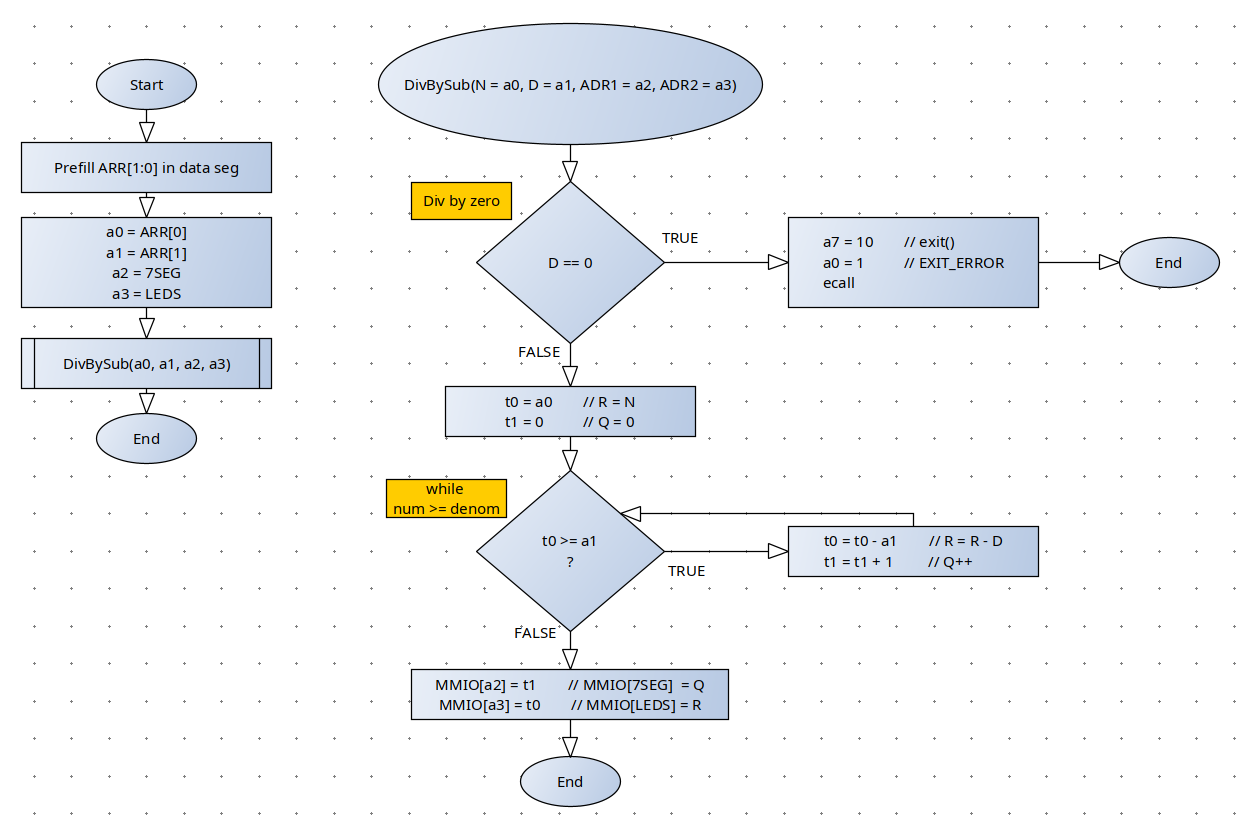
\includegraphics[width=0.9\textwidth]{../02_software/sw5/p1_flow.png}
					\caption{Flow chart for part 1}
					\label{fig:-02_software-sw5-p1_photos-flow-png}
				\end{figure}	

				\lstinputlisting[
					language={[riscv]Assembler},
					captionpos=top,
					caption={sw5\_p1.asm},
					breaklines=false]
					{../02_software/sw5/sw5_p1.asm}

			\subsubsection{Part 2}

				\begin{figure}[H]
					\centering
					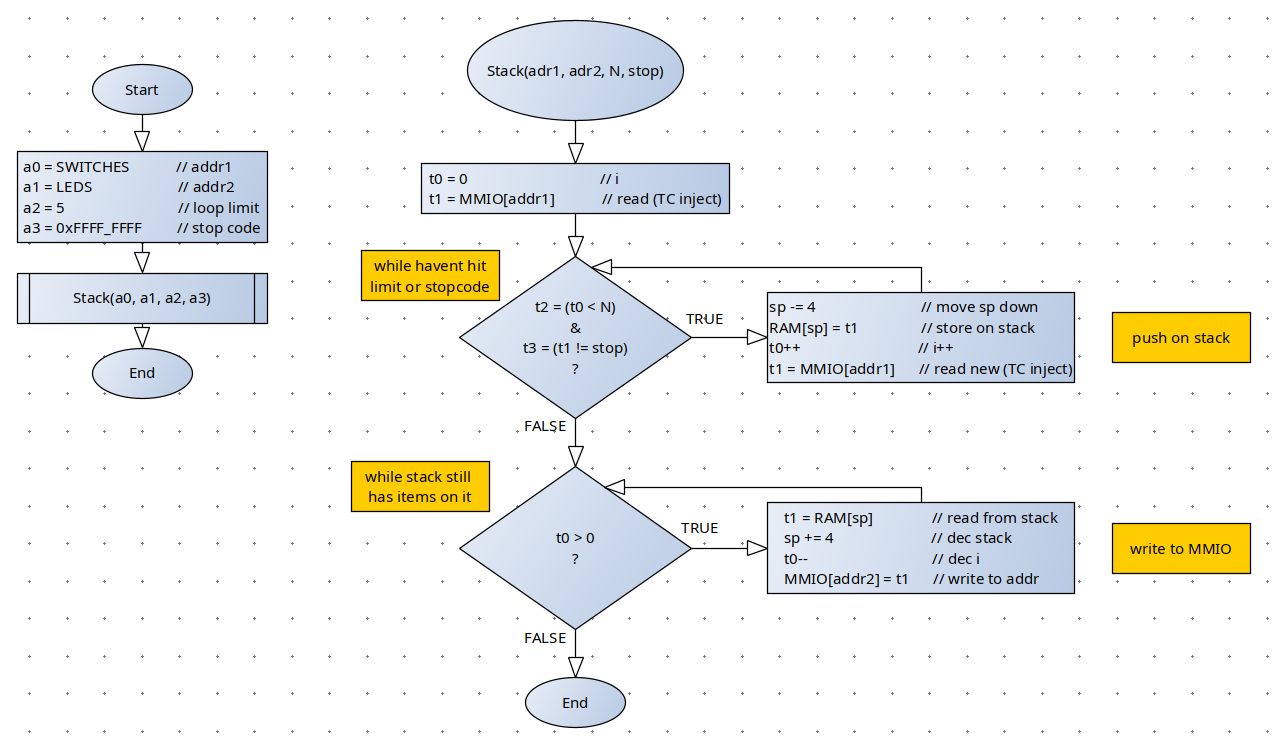
\includegraphics[width=\textwidth]{../02_software/sw5/p2_flow.png}
					\caption{Flow chart for part 2}
					\label{fig:-02_software-sw5-p2_photos-flow-png}
				\end{figure}	
				
				\lstinputlisting[
					language={[riscv]Assembler},
					captionpos=top,
					caption={Assembly code for sw5\_p2.asm},
					label={code:sw5p2},
					breaklines=false]
					{../02_software/sw5/sw5_p2.asm}

		\newpage
		\subsection{SW6 - Subroutines}
			\begin{figure}[H]
				\centering
				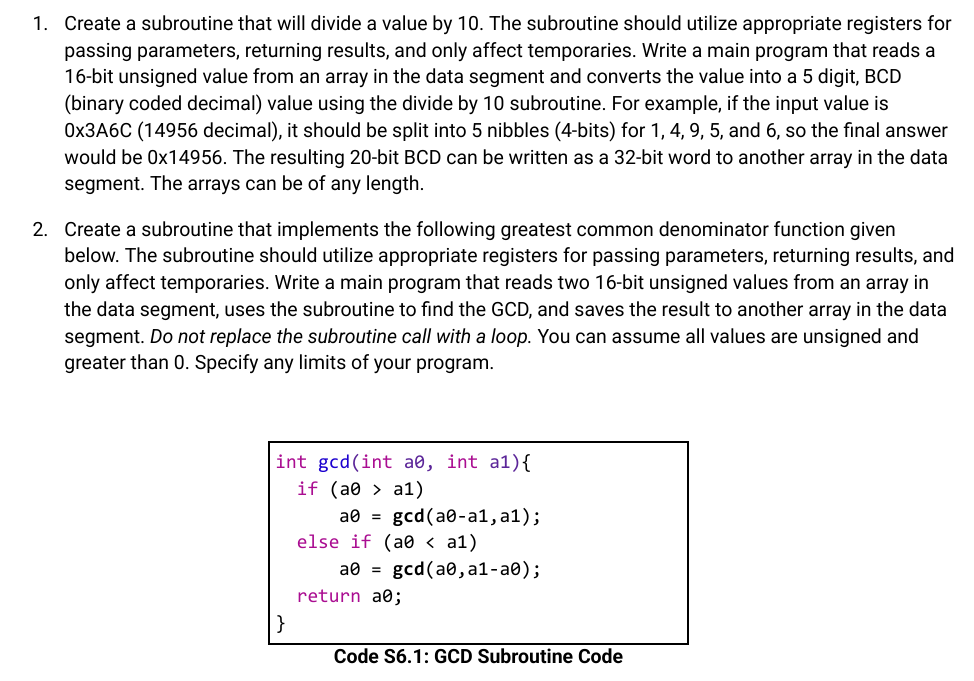
\includegraphics[width=0.8\textwidth]{../02_software/sw6/assignment.png}
				\caption{Questions to address}
				\label{fig:-02_software-sw6-assignment-png}
			\end{figure}

			\begin{figure}[H]
				\centering
				\includegraphics[width=0.6\textwidth]{../02_software/sw5/memconfig.png}
				\caption{Memory Map for this Assignment}
				\label{fig:-02_software-sw5-memconfig-png}
			\end{figure}


			\subsubsection{Part 1}

				\begin{figure}[H]
					\centering
					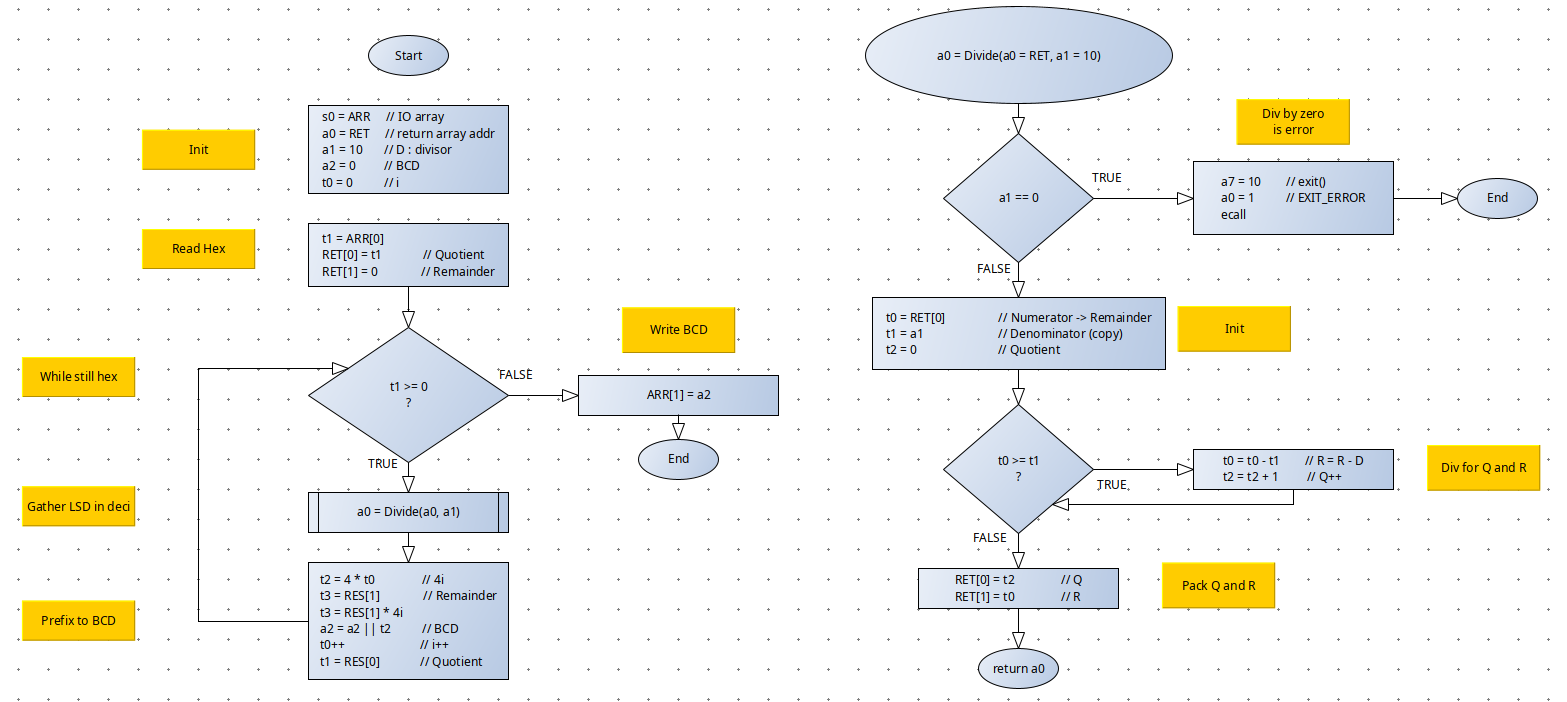
\includegraphics[width=0.9\textwidth]{../02_software/sw6/p1_flow.png}
					\caption{Flow chart for part 1}
					\label{fig:-02_software-sw6-p1_photos-flow-png}
				\end{figure}	

				\lstinputlisting[
					language={[riscv]Assembler},
					captionpos=top,
					caption={sw6\_p1.asm},
					breaklines=false]
					{../02_software/sw6/sw6_p1.asm}

			\subsubsection{Part 2}

				\begin{figure}[H]
					\centering
					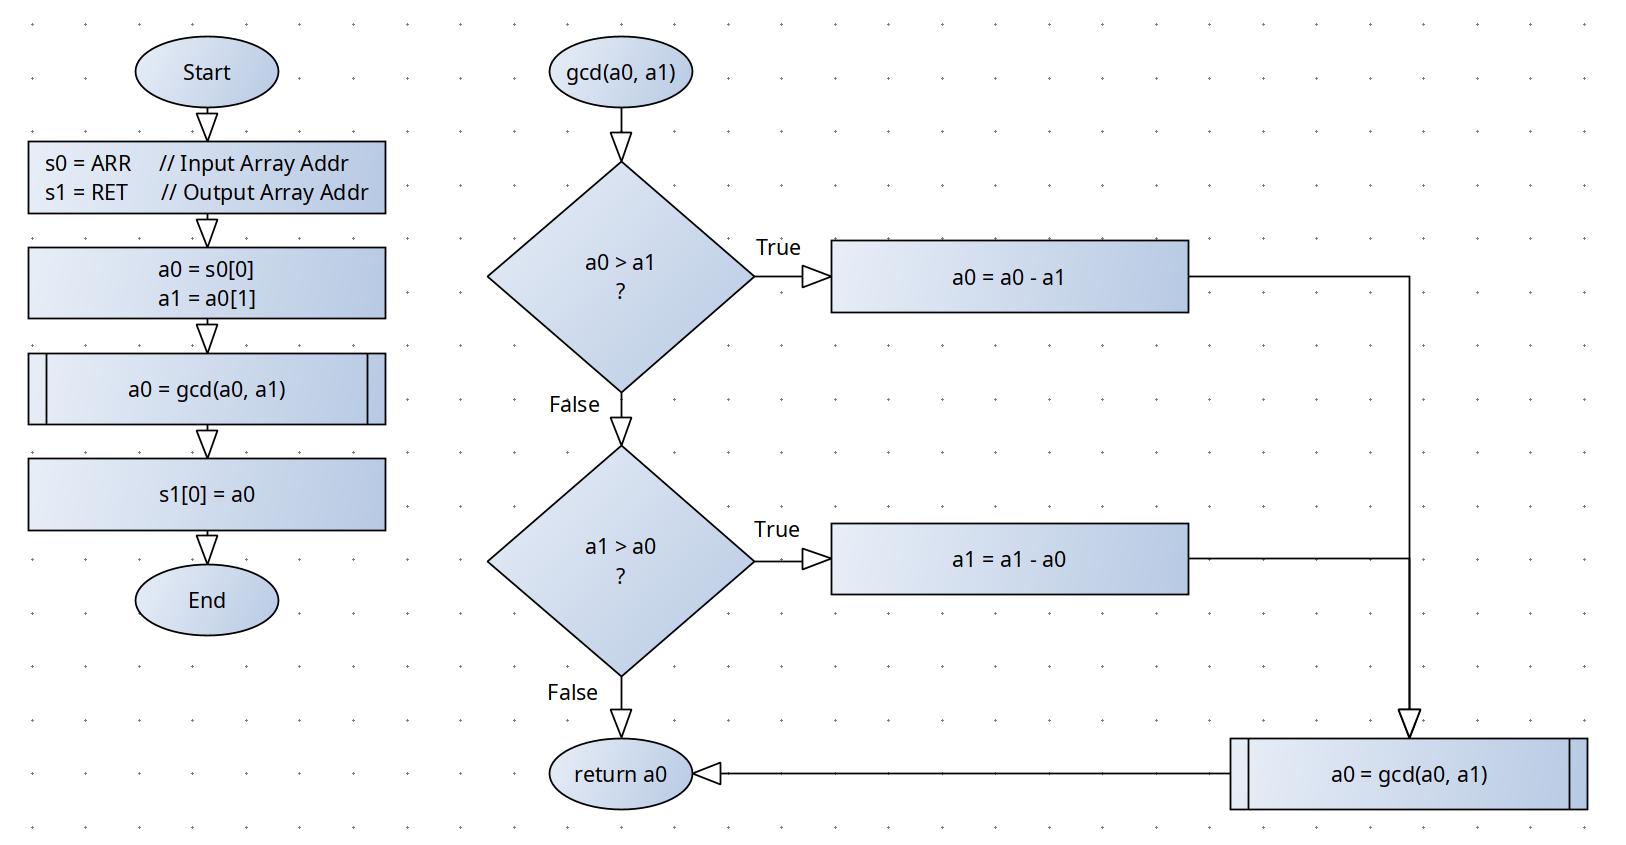
\includegraphics[width=\textwidth]{../02_software/sw6/p2_flow.png}
					\caption{Flow chart for part 2}
					\label{fig:-02_software-sw6-p2_photos-flow-png}
				\end{figure}	
				
				\lstinputlisting[
					language={[riscv]Assembler},
					captionpos=top,
					caption={Assembly code for sw6\_p2.asm},
					breaklines=false]
					{../02_software/sw6/sw6_p2.asm}

		\newpage
		\subsection{SW7 - Interrupts}
	
			Awkwardly enough, RARS doesn't support interrupts. This leaves me at 
			an impasse such that a polling 'main' function could be implemented using
			the \textit{Keyboard and Display MMIO Simulator} setting but that 
			won't use the CSR instructions I suspect what we want to use here. 
			BUT using CSR instructions ultimately means that the program wont be able 
			to be tested by RARS but only compiled into memory. For brevity, 
			I've opted to skip the RARS portion and map out the flow charts for now\ldots

			\begin{figure}[H]
				\centering
				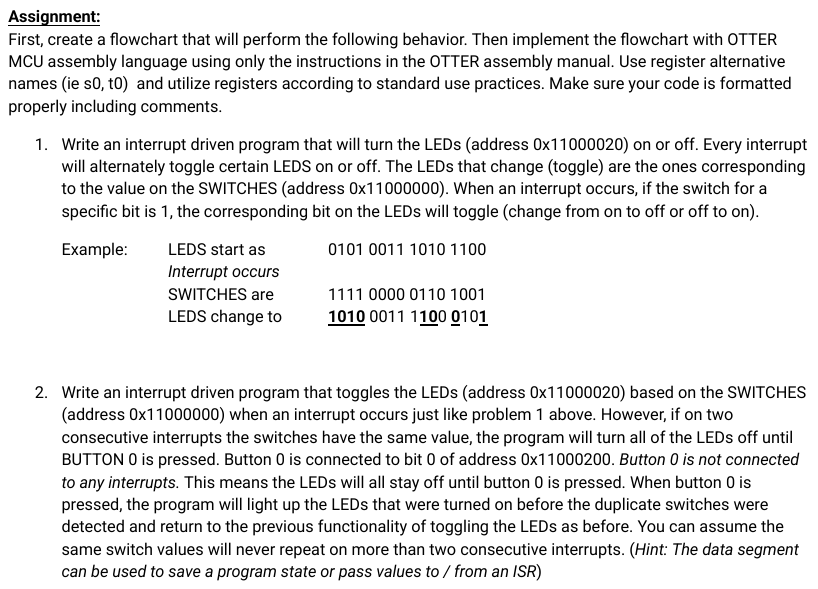
\includegraphics[width=0.8\textwidth]{../02_software/sw7/assignment.png}
				\caption{Questions to address}
				\label{fig:sw7-assign}
			\end{figure}
			

			\begin{figure}[H]
				\centering
				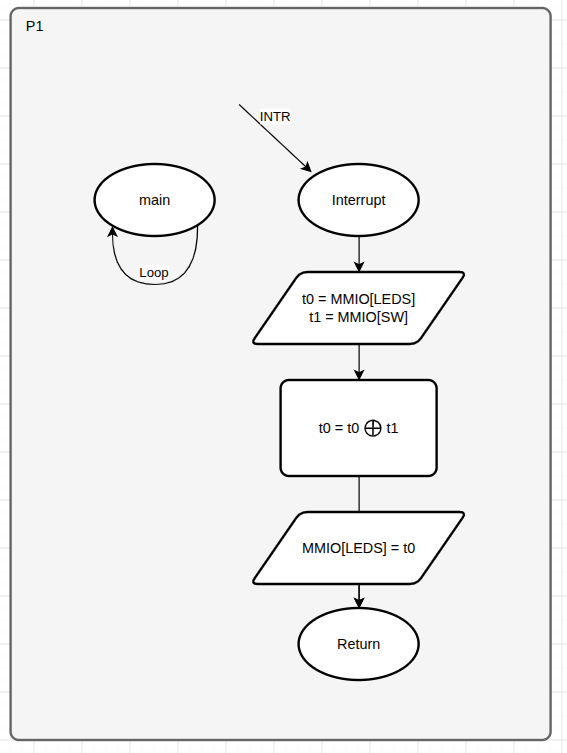
\includegraphics[width=0.6\textwidth]{../02_software/sw7/p1_flow.png}
				\caption{Flow chart for part 1}
				\label{fig:sw7-p1-flow}
			\end{figure}	

			\begin{figure}[H]
				\centering
				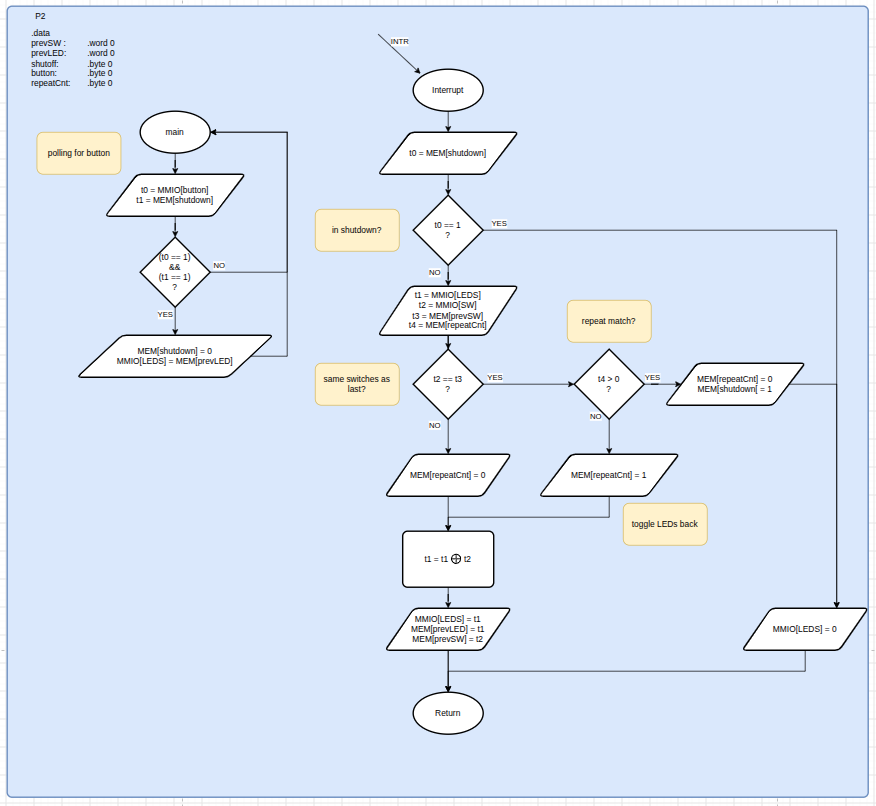
\includegraphics[width=\textwidth]{../02_software/sw7/p2_flow.png}
				\caption{Flow chart for part 2}
				\label{fig:sw7-p2-flow}
			\end{figure}	


	\newpage
	\section{Otter Code \& Test Sims}

		\subsection{Mux(s)}

			\lstinputlisting[
				language={Verilog},
				captionpos=top,
				caption={2 input Mux \texttt{Mux\_2N.sv}},
				breaklines=false,
				label={otter:mux2}
			]{../03_hardware/otter/src/Mux_2N.sv}

			\lstinputlisting[
				language={Verilog},
				captionpos=top,
				caption={4 input Mux \texttt{Mux\_4N.sv}},
				breaklines=false,
				label={otter:mux4}
			]{../03_hardware/otter/src/Mux_4N.sv}
	
			\lstinputlisting[
				language={Verilog},
				captionpos=top,
				caption={6 input Mux \texttt{Mux\_6N.sv}},
				breaklines=false,
				label={otter:mux6}
			]{../03_hardware/otter/src/Mux_6N.sv}
	
			\lstinputlisting[
				language={Verilog},
				captionpos=top,
				caption={TestSim for 6 input Mux \texttt{Mux\_6N\_tb.sv}},
				breaklines=false,
				label={ottertest:mux6}
			]{../03_hardware/otter/sim/Mux_6N_tb.sv}
	
		\newpage
		\subsection{Program Counter and Additives}

			\lstinputlisting[
				language={Verilog},
				captionpos=top,
				caption={Program Counter \texttt{PC\_Reg.sv}},
				breaklines=false,
				label={otter:pc}
			]{../03_hardware/otter/src/PC_Reg.sv}
		
			\lstinputlisting[
				language={Verilog},
				captionpos=top,
				caption={TestSim for Program Counter \texttt{PC\_Reg\_tb.sv}},
				breaklines=false,
				label={ottertest:pc}
			]{../03_hardware/otter/sim/PC_Reg_tb.sv}

			\lstinputlisting[
				language={Verilog},
				captionpos=top,
				caption={4+ PC Incrementer \texttt{Plus4\_1N.sv}},
				breaklines=false,
				label={otter:pc+4}
			]{../03_hardware/otter/src/Plus4_1N.sv}


		\newpage
		\subsection{Register File}

			\lstinputlisting[
				language={Verilog},
				captionpos=top,
				caption={Register File \texttt{RegFile.sv}},
				breaklines=false,
				label={otter:regfile}
			]{../03_hardware/otter/src/RegFile.sv}
		
			\lstinputlisting[
				language={Verilog},
				captionpos=top,
				caption={TestSim for Register File \texttt{RegFile\_tb.sv}},
				breaklines=false,
				label={ottertest:regfile}
			]{../03_hardware/otter/sim/RegFile_tb.sv}

		\newpage
		\subsection{Arithmetic Logic Unit}

			\lstinputlisting[
				language={Verilog},
				captionpos=top,
				caption={ALU \texttt{ALU.sv}},
				breaklines=false,
				label={otter:alu}
			]{../03_hardware/otter/src/ALU.sv}
		
			\lstinputlisting[
				language={Verilog},
				captionpos=top,
				caption={TestSim for ALU \texttt{ALU\_tb.sv}},
				breaklines=false,
				label={ottertest:alu}
			]{../03_hardware/otter/sim/ALU_tb.sv}

		\newpage
		\subsection{Immediate Generator}

			\lstinputlisting[
				language={Verilog},
				captionpos=top,
				caption={Immediate Gen \texttt{ImmedGen.sv}},
				breaklines=false,
				label={otter:immgen}
			]{../03_hardware/otter/src/ImmedGen.sv}
		
			\lstinputlisting[
				language={Verilog},
				captionpos=top,
				caption={TestSim for ImmedGen \texttt{ImmedGen\_tb.sv}},
				breaklines=false,
				label={ottertest:immgen}
			]{../03_hardware/otter/sim/ImmedGen_tb.sv}


		\newpage
		\subsection{Memory}

			\lstinputlisting[
				language={Verilog},
				captionpos=top,
				caption={Memory module \texttt{otter\_memory\_v1\_07.sv}},
				breaklines=false,
				label={otter:memory}
			]{../03_hardware/otter/src/otter_memory_v1_07.sv}

			\iffalse
			\lstinputlisting[
				language={Verilog},
				captionpos=top,
				caption={TestSim for ImmedGen \texttt{ImmedGen\_tb.sv}},
				breaklines=false,
				label={ottertest:immgen}
			]{../03_hardware/otter/sim/ImmedGen_tb.sv}
			\fi


		\newpage
		\subsection{Branch Address Generator}

			\lstinputlisting[
				language={Verilog},
				captionpos=top,
				caption={Branch Address Generator \texttt{BranchAddrGen.sv}},
				breaklines=false,
				label={otter:baddrgen}
			]{../03_hardware/otter/src/BranchAddrGen.sv}
		
			\lstinputlisting[
				language={Verilog},
				captionpos=top,
				caption={TestSim for Branch Addr Gen \texttt{BranchAddrGen\_tb.sv}},
				breaklines=false,
				label={ottertest:baddrgen}
			]{../03_hardware/otter/sim/BranchAddrGen_tb.sv}

		\newpage
		\subsection{Branch Condition Generator}

			\lstinputlisting[
				language={Verilog},
				captionpos=top,
				caption={Branch Condition Generator \texttt{BranchConditionGen.sv}},
				breaklines=false,
				label={otter:bcondgen}
			]{../03_hardware/otter/src/BranchConditionGen.sv}
		
			\lstinputlisting[
				language={Verilog},
				captionpos=top,
				caption={TestSim for Branch Condition Gen \texttt{BranchConditionGen\_tb.sv}},
				breaklines=false,
				label={ottertest:bcondgen}
			]{../03_hardware/otter/sim/BranchConditionGen_tb.sv}
			

		\newpage
		\subsection{Control Unit Decoder}

			\lstinputlisting[
				language={Verilog},
				captionpos=top,
				caption={Control Unit Decoder \texttt{CUnit\_Decoder.sv}},
				breaklines=false,
				label={otter:cudecoder}
			]{../03_hardware/otter/src/CUnit_Decoder.sv}
		
			\lstinputlisting[
				language={Verilog},
				captionpos=top,
				caption={TestSim for Control Unit Decoder \texttt{CUnit\_Decoder\_tb.sv}},
				breaklines=false,
				label={ottertest:cudecoder}
			]{../03_hardware/otter/sim/CUnit_Decoder_tb.sv}

		\newpage
		\subsection{Control Unit Finite State Machine}

			\lstinputlisting[
				language={Verilog},
				captionpos=top,
				caption={Control Unit FSM \texttt{CUnit\_FSM.sv}},
				breaklines=false,
				label={otter:cufsm}
			]{../03_hardware/otter/src/CUnit_FSM.sv}
		
			\lstinputlisting[
				language={Verilog},
				captionpos=top,
				caption={TestSim for Control Unit FSM \texttt{CUnit\_FSM\_tb.sv}},
				breaklines=false,
				label={ottertest:cufsm}
			]{../03_hardware/otter/sim/CUnit_FSM_tb.sv}


		\newpage
		\subsection{MicroController}

			\lstinputlisting[
				language={Verilog},
				captionpos=top,
				caption={Otter MCU \texttt{Otter\_MCU.sv}},
				breaklines=false,
				label={otter:mcu}
			]{../03_hardware/otter/src/Otter_MCU.sv}
		
			\lstinputlisting[
				language={Verilog},
				captionpos=top,
				caption={TestSim for MCU, \texttt{CUnit\_FSM\_tb.sv}, using RARS from \texttt{demo.asm}},
				breaklines=false,
				label={ottertest:mcu}
			]{../03_hardware/otter/sim/Otter_MCU_tb.sv}


		\newpage
		\subsection{Seven Segment}

			\lstinputlisting[
				language={Verilog},
				captionpos=top,
				caption={Binary-Coded Decimal\texttt{BCD.sv}},
				breaklines=false,
				label={otter:bcd}
			]{../03_hardware/otter/src/BCD.sv}

			\lstinputlisting[
				language={Verilog},
				captionpos=top,
				caption={\texttt{CathodeDriver.sv}},
				breaklines=false,
				label={otter:catho}
			]{../03_hardware/otter/src/CathodeDriver.sv}

			\lstinputlisting[
				language={Verilog},
				captionpos=top,
				caption={Seven Segment Display Driver \texttt{SevSegDisp.sv}},
				breaklines=false,
				label={otter:seven}
			]{../03_hardware/otter/src/SevSegDisp.sv}

		\newpage
		\subsection{Peripheral Fabric}
		
			\lstinputlisting[
				language={Verilog},
				captionpos=top,
				caption={Otter Wrapper \texttt{OTTER\_Wrapper\_v1\_02.sv}},
				breaklines=false,
				label={otter:wrap}
			]{../03_hardware/otter/src/OTTER_Wrapper_v1_02.sv}

			\lstinputlisting[
				language={Verilog},
				captionpos=top,
				caption={Visual testsim for Otter Wrapper \texttt{OTTER\_Wrapper\_tb.sv}},
				breaklines=false,
				label={ottertest:wrap}
			]{../03_hardware/otter/sim/OTTER_Wrapper_tb.sv}

			\lstinputlisting[
				language={Verilog},
				captionpos=top,
				caption={Peripheral Bindings \texttt{Basys3\_Master.xdc}},
				breaklines=true,
				label={otter:constraint}
			]{../03_hardware/otter/constraint/Basys3_Master.xdc}


		\newpage
		\subsection{Interrupts}
		
			\lstinputlisting[
				language={Verilog},
				captionpos=top,
				caption={Debounce OneShot \texttrademark \texttt{OneShot.sv}},
				breaklines=false,
				label={otter:debounce}
			]{../03_hardware/otter/src/OneShot.sv}

			\lstinputlisting[
				language={Verilog},
				captionpos=top,
				caption={Testsim for debounce OneShot \texttrademark \texttt{OneShot\_tb.sv}},
				breaklines=false,
				label={ottertest:debounce}
			]{../03_hardware/otter/sim/OneShot_tb.sv}

			\lstinputlisting[
				language={Verilog},
				captionpos=top,
				caption={Control Status Register \texttt{ControlStatusRegister.sv}},
				breaklines=false,
				label={otter:csr}
			]{../03_hardware/otter/src/ControlStatusRegister.sv}

			\lstinputlisting[
				language={Verilog},
				captionpos=top,
				caption={Testsim for Control Status Register \texttt{ControlStatusRegister\_tb.sv}},
				breaklines=false,
				label={ottertest:csr}
			]{../03_hardware/otter/sim/ControlStatusRegister_tb.sv}
			
			\lstinputlisting[
				language={[riscv]Assembler},
				captionpos=top,
				caption={Hardware Interrupt Test \texttt{InterruptTestProg.asm}},
				breaklines=false,
				label={ottertest:interrupt}
			]{../03_hardware/hw8/InterruptTestProg.asm}

\end{document}
